\documentclass[a4paper]{article}

\usepackage{CJK} %设置中文包
\usepackage{listings}  % 用于代码插入
\usepackage{xcolor} % 用于配色
\usepackage[landscape,  margin=2cm, headsep=.3cm]{geometry}
\usepackage{graphicx} %使用图形
\usepackage{amsmath} %使用数学库


\usepackage{multicol} %设置多栏
\usepackage{lipsum}% dummy text
\setlength{\columnseprule}{0.1pt} %设置栏之间的分隔线的宽度,0则不显示分隔线。
\setlength{\columnsep}{0.7cm} %设置栏之间的间隔。

\usepackage[linktocpage=false, colorlinks, linkcolor=black, anchorcolor=black, citecolor=black]{hyperref}
\hypersetup{CJKbookmarks=true}


\usepackage{fancyhdr}
\pagestyle{fancy}
\fancypagestyle{plain}{
  \pagestyle{fancy}
}

%对齐方式
%左对齐 \begin{flushleft}...\end{flushleft}搜索
%居中 \begin{center}...\end{center}
%右对齐 \begin{flushright}...\end{flushright}

%打印公式符号
% 打印 % => \%
% 打印 ^ => \^{}
% 打印 _ => \_
%     + => \#
%     $ => \$
%     { => \{
%     } => \}
%     ~ => \~ ,推荐 $\sim$
%     & => \&
%     | => $|$
%     < => $<$
%     > => $>$
%     * => $*$
%


%页眉和页脚的左部,中部,右部
\lhead{\thepage}
\chead{\textit{NENU CS ACM 模板}}
\rhead{\thepage}
\lfoot{\thepage}
\cfoot{make by tiankonguse powered by $vici$ v0.7}
\rfoot{\thepage}
\renewcommand{\headrulewidth}{0.2pt}
\renewcommand{\footrulewidth}{0pt}

%定义一个名为 darkgreen 的颜色
\xdefinecolor{darkgreen}{rgb}{0,0.35,0}
%设置插入的代码的样式
\lstset{
    tabsize=4,%tab键用四个空格替换
    basicstyle=\ttfamily\scriptsize,
    extendedchars=false, %解决代码跨页时,章节标题,页眉等汉字不显示的问题
  	escapechar=`, %中文添加`后,可以避免注释中如果含有中文则顺序错乱
    breaklines=true,      %让LaTeX自动将长的代码行换行排版
    breakatwhitespace=false,
    language=C++,   %让LaTeX排版时将C++键字突出显示
    keywordstyle=\textbf, %for printing
    morekeywords={bool,__int64},
    keywordstyle=\color{blue!90},%关键词的颜色
    commentstyle=\color{darkgreen!85},%注释的颜色
    rulesepcolor=\color{red!20!green!20!blue!20},
    basicstyle=\footnotesize\ttfamily, %for paste
    columns=flexible,
    xrightmargin=0.5em %右边距
}


\begin{document}

%使用CJK中文 ,仿宋格式
\begin{CJK*}{UTF8}{gbsn}

%首页是封面,所以应该显示一栏
\begin{onecolumn}

%插入图片
\begin{figure}
	\centering{
		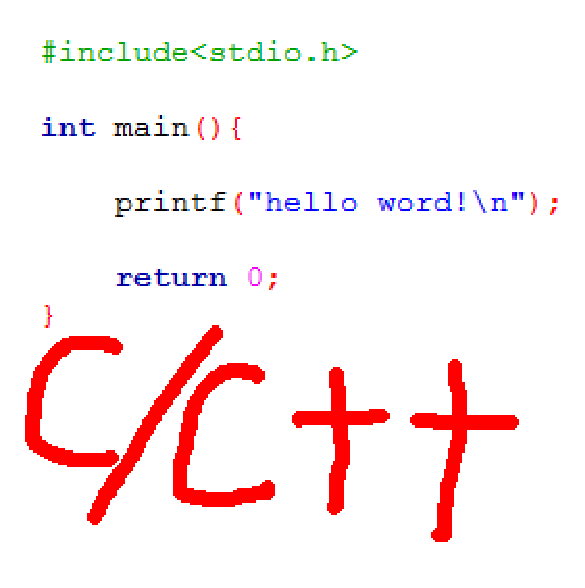
\includegraphics[width=10cm]{front.eps}
	}\\
\end{figure}

%插入文本
%linespread 设置行距
\linespread{4}{
	\centering{
		\fontsize{30pt}{\baselineskip}\selectfont {
		
		%
		
			ACM 模板 
			
		%
		
		}
	}
}

%插入文本
\linespread{2}{
	\centering{
		\fontsize{10pt}{\baselineskip}\selectfont {
		
%

make by tiankonguse(http://tiankonguse.com/)\\powered by vici

%

		}
	}
}

\end{onecolumn}

%新的一页
\clearpage

this is a blank page.

%新的一页
\clearpage

%设置多栏
\begin{multicols}{3}

%\begin{tabular}{p{0.9\columnwidth}}

%设置目录的名字
\renewcommand{\contentsname}{目录}

%生成目录
\tableofcontents

\clearpage 



%全部左对齐
\begin{flushleft} 

% 
% section{一级目录}
%
% 
%subsection{二级目录}
%
%\begin{lstlisting}[language={代码语言}]
% 插入代码
%  //`代码注释全部用这个引起来,防止因为中文引起顺序错乱`
%\end{lstlisting}

\section{Base}

\subsection{头文件}
\begin{lstlisting}
#include <iostream>
#include <cstdio>
#include <cstdlib>
#include <cstring>
#include <algorithm>
#include <cmath>
#include <string>
#include <vector>
#include <queue>
#include <set>
#include <map>
#include <ctime>
#include <map>
#include <set>
#include <deque>
#include <stack>
#include <functional>
using namespace std;

#ifdef __int64
typedef __int64 LL;
#else
typedef long long LL;
#endif

const int inf = 0x3f3f3f3f;
const LL Inf = 0x3FFFFFFFFFFFFFFFLL
int main(){

    return 0;
}
\end{lstlisting}


\subsection{文件结束符}
\begin{lstlisting}
`windows : ctrl-z`
`linux : ctrl-d`
\end{lstlisting}

\subsection{codeblock配置终端}
\begin{lstlisting}
`setting `
`	->environment`
`	->gerneral setting:`
`	->Termial to lunch console programs:`
`	-> gnome-terminal -x`
\end{lstlisting}

\subsection{codeblock快捷键}
\begin{lstlisting}
`按住Ctrl滚滚轮,代码的字体大小。`
`在编辑区按住右键可拖动代码,省去拉滚动条之麻烦;相关设置:Mouse Drag Scrolling。` 
`Ctrl+D可复制当前行或选中块。`
`Ctrl+Shift+C注释掉当前行或选中块`
`Ctrl+Shift+X则解除注释。 `
`Tab缩进当前行或选中块,Shift+Tab减少缩进。`
`可拖动选中块使其移动到新位置,按住Ctrl则为复制到新位置。`
`按下Atl,再拖动鼠标,可以实现部分选择。`
`F2和Shift+F2分别可以显隐下方Logs \& others栏和左方的Management栏。`
\end{lstlisting}

\subsection{通用long long}
\begin{lstlisting}
#ifdef __int64
typedef __int64 LL;
#else
typedef long long LL;
#endif
\end{lstlisting}

\subsection{设置栈的大小}
\begin{lstlisting}
//Increase the Stack Size(Only C++)
#pragma comment(linker, "/STACK:36777216")
\end{lstlisting}


\subsection{Notes}
\begin{lstlisting}
double pi = 3.14159265358...; // no 'f' appended
#define maxn 200 + 20 // it's not safe
int const mod = 1000000007; // use "const" to accelerate
judge ``mp.find(x) != mp.end()" is better than ``ret += mp[x]" directly

0x3f3f3f3f   =   1061109567  (recommended)
0x7f7f7f7f   =   2139062143
0x3FFFFFFFFFFFFFFFLL    =   4611686018427387903    (recommended)
0x7FFFFFFFFFFFFFFFLL    =   9223372036854775807


//memset
memset(dpMin, 0x3f, sizeof(dpMin)); //  inf
memset(dpMax, 0xc0, sizeof(dpMax)); // -inf
//for_bit
for (int i = a ; i != 0 ; i = (i - 1) & a)
//count bit
static int countbit[1024];
for (int i = 1; i < 1024; ++i) countbit[i] = 1 + countbit[i - ((i ^ (i - 1)) & i)];
//sort by lexicographic
int cmp(const void *a, const void *b) {
	char *x = (char *)a;
	char *y = (char *)b;
	return strcmp(x, y);
}
qsort(str, n, sizeof(str[0]), cmp);
\end{lstlisting}


\section{数据结构}

\subsection{数的范围}
\begin{lstlisting}[language={c++}]
int  2147483647; 10^9
int   -2147483648;
long long  9223372036854775807; 10^18
long long   -9223372036854775808;
sqrt(INT_MAX)=46340
\end{lstlisting}

\subsection{素数专题}
\begin{lstlisting}[language={c++}]
`素数定理:pi(x)/x*ln(x)=1,pi(x)表示小于x的素数的个数`
`孪生素数猜想:存在无穷个p,p+2的素数对`
`PS:陈景润证明的存在无穷个素数p,p+2至多有两个素数因子,及传说当中的"1+2"问题`
`哥德巴赫猜想:每个大于2的偶数是两个素数的和`
`n\^2{}+1猜想:存在无穷个n\^2{}+1这样形式的素数`
`埃拉托斯尼斯筛法:正整数n是素数,当且仅当它不能被任何小于n的平方根的素数整除。`
`有时候素数的范围很大,不能把所有的素数表打出来,就要只存部分素数。 `
`如果求区间的素数,就对区间进行筛法`
\end{lstlisting}


\subsubsection{素数表基本晒法}
\begin{lstlisting}[language={c++}]
const int N=1000000;
const int M=300000;
bool is[N]; 
int prm[M];
int getprm(){
	int e = (int)(sqrt(0.0 + N) + 1),k=0,i;
	memset(is, 1, sizeof(is));
	prm[k++] = 2; is[0] = is[1] = 0;
	for (i = 4; i < N; i += 2) is[i] = 0;
	for(i=3;i<e;i+=2){
		if(is[i]){
			prm[k++]=i;
			for(int s=i+i,j=i*i;j<N;j+=s)is[j]=0;
		}
	}
	for (; i < N; i += 2)
		if (is[i])prm[k++] = i;
	return k; 
}
\end{lstlisting}

\subsubsection{压位筛素数}
\begin{lstlisting}[language={c++}]
typedef long long LL;
LL NN = 2147483647LL;
const int N= (2147483647>>3)+1;
const int M=14630853;
char is[N];
LL prm[M];
void setIs(int pos){
    is[pos>>3] &= ~(1<<(pos%8));
}

bool getIs(int pos){
    return is[pos>>3] & (1<<(pos%8));
}

int getprm(){
	int e = (int)(sqrt(0.0 + NN) + 1),k=0,i;
	memset(is, 0XFF, sizeof(is));

	prm[k++] = 2;
	setIs(0);
	setIs(1);
	for (i = 4; i < NN; i += 2){
        setIs(i);
	}

	for(i=3;i<e;i+=2){
		if(getIs(i)){
			prm[k++]=i;
			for(int s=i+i,j=i*i;j<NN;j+=s){
                setIs(j);
			}
		}
	}
	for (; i < NN; i += 2)
		if (getIs(i))prm[k++] = i;
	return k;
}
\end{lstlisting}

\subsubsection{sieve}
\begin{lstlisting}
//cnt[1e7] = 664579, cnt[1e6] = 78498
//mark[i] : the minimum factor of i (when i is a prime, mark[i] == i)
int const maxn = 1e7;
int pri[maxn], mark[maxn], cnt;
void sieve() {
	cnt = 0, mark[0] = mark[1] = 1;
	for (int i = 2; i < maxn; i++) {
		if (!mark[i]) pri[cnt++] = mark[i] = i;
		for (int j = 0; pri[j] * i < maxn; j++) {
			mark[ i * pri[j] ] = pri[j];
			if (i % pri[j] == 0) break;
		}
	}
}
\end{lstlisting}

\subsubsection{小舟学长的筛法}
\begin{lstlisting}[language={c++}]
const int N=1000000;
const int M=300000;
int mark[N];//`最小因子`
int prm[M];
int cnt;

int getprm(){
	int j,i;
	memset(mark, 0, sizeof(mark));

    cnt = 0;
    mark[0] = mark[1] = 1;

    for(i = 2; i < N; ++i){
        if(!mark[i]){
            prm[cnt++] = mark[i] = i;
        }
        for(j=0;prm[j]*i<N;++j){
            mark[i*prm[j]] = prm[j];
            if(i%prm[j] == 0)break;
        }
    }
    return cnt;
}
\end{lstlisting}

\subsubsection{区间素数}
\begin{lstlisting}[language={c++}]
bool _is[N];
int _prm[N], _num;
void rangePrime(LL L, LL U) {
    LL i,k,size=U-L,tmp;
    _num = 0;
    memset(_is,1,sizeof(_is));

    for(i=0; i <= num && prm[i]*prm[i]<=U; ++i) {
        k = (L + prm[i] - 1)/prm[i];
        while(k <= 1) {
            k++;
        }
        tmp = k*prm[i];
        while(tmp <= U) {
            _is[tmp - L] = 0;
            tmp += prm[i];
        }
    }

    for(i = 0; i <= size; ++i) {
        if(_is[i]) {
            _prm[_num++]=i+L;
        }
    }
}
\end{lstlisting}

\subsubsection{sieve 100000 primes $>$ 1e12}
\begin{lstlisting}
//or java.BigInteger -> nextProbablePrime();
typedef long long ll;
int const maxn = 4e6;
ll const start = 1e12, end = start + 3e6;

int pri[maxn], cnt; bool mark[maxn];
ll pl[maxn]; int pnt; bool markl[maxn];

void __sieve_large() {
    cnt = 0, mark[0] = mark[1] = true;
    for (int i = 2; i < maxn; ++i) {
        if (!mark[i]) pri[cnt++] = i;
        for (int j = 0; i * pri[j] < maxn; ++j) {
            mark[i * pri[j]] = true;
            if (!(i % pri[j])) break;
        }
    }
    ll pos;
    for (int i = 0; i < cnt; ++i) {
        if (start % pri[i] == 0) pos = start;
        else pos = start - start % pri[i] + pri[i];
        for (; pos <= end; pos += pri[i]) {
            markl[pos - start] = true;
        }
    }
    pnt = 0;
    for (int i = 0; i <= end - start; ++i) {
        if (!markl[i]) pl[pnt++] = start + i;
    }
}
\end{lstlisting}

\subsubsection{反素数}

\begin{lstlisting}[language={c++}]
`对于任何正整数x,其约数的个数记做g(x).`
`例如g(1)=1,g(6)=4.`
`如果某个正整数x满足:对于任意i(0$<$i$<$x),都有g(i)$<$g(x),则称x为反素数.`
`反素数可以理解为对于x,在[1,x]中,x的约数最多,也就是当前约数最多的值。`

int rprim[35][2] = {498960,200,332640,192,277200,180, 
221760,168,166320,160,110880,144,83160,128,55440,120,
50400,108,45360,100,27720,96,25200,90,20160,84,15120,
80,10080,72,7560,64,5040,60,2520,48,1680,40,1260,36,
840,32,720,30,360,24,240,20,180,18,120,16,60,12,48,
10,36,9,24,8,12,6,6,4,4,3,2,2,1,1};

typedef __int64 INT;
INT bestNum;   //`约数最多的数`
INT bestSum;   //`约数最多的数的约数个数`
const int M=1000; //`反素数的个数 `
INT n=500000;//`求n以内的所有的反素数`
INT rprim[M][2];
//`2*3*5*7*11*13*17>n,所以只需考虑到17即可`
INT sushu[14]={2,3,5,7,11,13,17,19,23,29};  

//`当前走到num这个数,接着用第k个素数,num的约数个数为sum,`
//`第k个素数的个数上限为limit`
void getNum(INT num,INT k,INT sum,INT limit)  {
 	if(num>n)return;
	if(sum>bestSum){
		bestSum = sum,bestNum = num;;
	}else if(sum == bestSum && num < bestNum){  
		//`约数个数一样时,取小数`
		bestNum = num;
	}

	//`只需考虑到素数17,即sushu[6]`
	if(k>=7) return; 
	
	//`素数k取i个`
	for(INT i=1,p=1;i<=limit;i++){   
		p*=sushu[k];
		getNum(num*p,k+1,sum*(i+1),i);
	}
}
//`求大于等于log2(n)的最小整数`
INT log2(INT n){  
	INT i = 0,p = 1;
	while(p<n){p*=2,i++;}
	return i;
}
int getrprim(){
	int i = 0;
	while(n>0){
		bestSum =bestNum = 1;
		getNum(1,0,1,log2(n));
		n = bestNum - 1;
		rprim[i][0]=bestNum;
		rprim[i][1]=bestSum;
		i++;
	}
	return i;	
}
\end{lstlisting}


\subsection{大素数}
\begin{lstlisting}[language={c++}]
`pow\_mod 见x\^{}n mod c非递归版`
`muti\_mod 见(a*b) mod c`
`cons int S=20; 越大正确率越大`
`factor是一个向量,储存N的素数因子`
\end{lstlisting}


\subsubsection{素数测试的GCD}
\begin{lstlisting}[language={c++}]
LL gcd(LL a,LL b){
    if (a==0 || b == 0) return 1;
    a = abs(a);
    b = abs(b);
    while (b){
        LL t=a%b; a=b; b=t;
    }
    return a;
}
\end{lstlisting}

\subsubsection{检验n是不是合数}
\begin{lstlisting}[language={c++}]
//`以a为基,n-1=x*2\^{}t`
bool check(LL a,LL n,LL x,LL t){   
    LL ret=pow_mod(a,x,n),last=ret;
    for (int i=1;i<=t;i++){
        ret=muti_mod(ret,ret,n);
        if (ret==1 && last!=1 && last!=n-1) return 1;
        last=ret;
    }
    if (ret!=1) return 1;
    return 0;
}
\end{lstlisting}



\subsubsection{大素数测试}
\begin{lstlisting}[language={c++}]
bool Miller_Rabin(LL n){
    LL x=n-1,t=0;
    while ((x&1)==0) x>>=1,t++;
    bool flag=1;
    if (t>=1 && (x&1)){
        for (int k=0;k<S;k++){//s=20
            LL a=rand()%(n-1)+1;
            if (check(a,n,x,t)) {flag=1;break;}
            flag=0;
        }
    }
    if (!flag || n==2) return 0;
return 1;   
}
\end{lstlisting}

\subsubsection{pollard\_rho分解}
\begin{lstlisting}[language={c++}]
//` 得到一个因数.返回N时为一个没有找到 `
LL Pollard_rho(LL x,LL c){
    LL i=1,x0=rand()%x,y=x0,k=2;
    while (1){
        i++;
        x0=(muti_mod(x0,x0,x)+c)%x;
        LL d=gcd(y-x0,x);
        if (d!=1 && d!=x)return d;
        if (y==x0) return x;
        if (i==k)y=x0,k+=k;
    }
}
\end{lstlisting}


\subsubsection{质因数分解N }
\begin{lstlisting}[language={c++}]
void findfac(LL n){           
    if (!Miller_Rabin(n)){
        factor.push_back(n);//`factor为一个向量`
        return;
    }
    LL p=n;
    while (p>=n) p=Pollard_rho(p,rand() % (n-1) +1);
    findfac(p);
    findfac(n/p);
}
\end{lstlisting}


\subsection{梅森素数}
\begin{lstlisting}[language={c++}]
`m是一个素数,$M=2^m-1$也是一个素数,则M是梅森素数。`
`使用大素数测试得到森素数。`
\end{lstlisting}



\subsection{费马小定理}
\begin{lstlisting}[language={c++}]
`如果p是素数,则$a^{p − 1}$ ≡ $1(mod p)$对所有整数a都成立`
\end{lstlisting}



\subsection{欧拉函数}

\subsubsection{欧拉原理}
\begin{lstlisting}[language={c++}]
`$a^{phi(n)}$ ≡  1 (mod n) gcd(a, n) = 1`
\end{lstlisting}

\subsubsection{一些结论}
\begin{lstlisting}[language={c++}]
`a为N的质因数`
`若 (N/a)\%a == 0 则有 E(N) = E(N/a)*a.`
`若 (N/a)\%a !=0则有 E(N) = E(N/a)*(a-1)`
`一个数的所有质因子之和 F(n)*n/2.`
\end{lstlisting}


\subsubsection{第n个与m互质的数}
\begin{lstlisting}[language={c++}]
`如果求与m互质的第n个数,可以先把小于m的互质的数错在ans中(筛法求)`
`(从1开始存,最后一个存在0中),然后大于m的互质的数都是小于m的互质的数加上若干个m得到的。`
int euler(int n,int m){
    memset(map,true,sizeof(map));
    int i=0,num=n;
    for(;num!=1; i++;){
        if(num%prim[i]==0){
            while(num%prim[i]==0)num/=str[i];
            for(int j=prim[i];j<=n;j+=prim[i]){
                map[j]=false;
            }
        }
    }
    num=0;
    for(i=1;i<n;i++){
        if(map[i]){
            ans[++num]=i;
        }
    }
    ans[0]=ans[num];
    return ans[m%num]+(m-1)/num * n;
}
\end{lstlisting}

\subsection{sieve phi}
\begin{lstlisting}
int const maxn = 1e6;
int pri[maxn], cnt;
int phi[maxn];
void __sieve_phi() {
    cnt = 0, phi[1] = 1;
    for (int i = 2; i < maxn; ++i) {
        if (!phi[i]) {
            pri[cnt++] = i;
            phi[i] = i - 1;
        }
        for (int j = 0; pri[j] * i < maxn; ++j) {
            if (!(i % pri[j])) {
                phi[i * pri[j]] = phi[i] * pri[j];
                break;
            }
            else {
                phi[i * pri[j]] = phi[i] * (pri[j] - 1);
            }
        }
    }
}
\end{lstlisting}

\subsubsection{打表欧拉函数}
\begin{lstlisting}[language={c++}]
`这个表存的是小于N的数的欧拉函数`
const int N=10000; 
int phi[N+1]; 
void ruler(){ 
	int i,j; 
	for (i = 1; i <= N; i++) phi[i] = i;
	for (i = 2; i <= N; i += 2) phi[i] /= 2;
	for (i = 3; i <= N; i += 2) 
		if(phi[i] == i) {
			for (j = i; j <= N; j += i)
				phi[j] = phi[j] / i * (i - 1);
		}
} 
\end{lstlisting}


\subsubsection{单独求欧拉函数(公式)}
\begin{lstlisting}[language={c++}]
int euler(int x){//` 就是公式`
	int i, res=x;
	int max= (int)sqrt(x * 1.0) + 1; 
	for (i = 2; i <max; i++)
		if(x%i==0) {
		res = res / i * (i - 1);
		while (x % i == 0) x /= i; //` 保证i一定是素数`
		}
	if (x > 1) res = res / x * (x - 1);
	return res;
}
\end{lstlisting}


\subsubsection{容斥求小于a的与n互质的个数}
\begin{lstlisting}[language={c++}]
`str[n].count为n的质数因子的个数`
`Str[n].prim[]中存的就是质数因子`
`这个不能用简单的容斥,因为这里的除法不是全部能整除,用简单的容斥是错的。`
LL myrongchi(int index,int a,int n){
	LL r=0,t;
	for(int i=index;i<str[n].count;i++){
		t=a/str[n].prim[i];
		r+=t-myrongchi(i+1,t,n);
	}
	return r;	
}
\end{lstlisting}

\subsection{随机数}

\subsubsection{设置随机种子}
\begin{lstlisting}[language={c++}]
srand(time(NULL));
\end{lstlisting}

\subsubsection{产生随机数}
\begin{lstlisting}[language={c++}]
rand();
\end{lstlisting}




\subsection{二分}

\subsubsection{最大值最小化问题}
\begin{lstlisting}[language={c++}]
`m个正整数的序列划分成m个子连续序列,每个子序列的个数字之和为S, 使所有S中的最大S最小。`
\end{lstlisting}


\subsubsection{数轴上点到点的距离和}
\begin{lstlisting}[language={c++}]
`点的中位数就是答案`
`如果点有奇数个,答案唯一。`
`如果点有偶数个,答案是个区间`
\end{lstlisting}

\subsubsection{数轴上点到点的距离平方和}
\begin{lstlisting}[language={c++}]
`列出方程后,可以证明是个凸函数。`
`于是这个可以使用三分做。`
`猜想可能还是中位数。`
\end{lstlisting}

\subsubsection{坐标系上点到点的曼哈顿距离和}
\begin{lstlisting}[language={c++}]
`此时,x轴与y轴没有关系了,找到x轴的中位数与y轴的中位数即可。`
\end{lstlisting}

\subsubsection{...到点的距离平方和}
\begin{lstlisting}[language={c++}]
`这个经过列出等式后,可以发现,每一维是相互独立的。`
`而转化成了在数轴上的距离平方和问题了。`
\end{lstlisting}

\subsubsection{...到点的距离和}
\begin{lstlisting}[language={c++}]
`这个需要偏导数理论。`
`写出偏导数后发现当其他维数固定时,这个维数还是相互独立的。`
`但是不使用偏导数时,我们只需使用变步长寻找即可。`
`例如:`
`1. 取步长为step,起点为(x0,y0)`
`2. 我们找到上下左右的四个点的值,如果有比(x0,y0)更优的值,则更新(x0,y0)。`
`3. 循环执行步骤2,直到(x0,y0)就是最优值。`
`4. 此时,步长变为原来的0.5倍,继续执行步骤2.直到step达到一定的精度。`
\end{lstlisting}

\subsubsection{...到直线的距离和}
\begin{lstlisting}[language={c++}]
`思考中`
\end{lstlisting}


\subsubsection{...到直线的距离平方和}
\begin{lstlisting}[language={c++}]
`思考中`
\end{lstlisting}



\subsection{贪心}

\subsubsection{区间选点问题}
\begin{lstlisting}[language={c++}]
`取尽量少的点,使每个区间内都至少有一个点。`
\end{lstlisting}

\subsubsection{区间覆盖问题}
\begin{lstlisting}[language={c++}]
`数轴上有若干区间,选尽量少的区间,覆盖指定区间。`
\end{lstlisting}



\subsection{GCD}


\subsubsection{普通求公约数}
\begin{lstlisting}[language={c++}]
LL gcd(LL x,LL y){
	if(!x || !y)return x?x:y;
	for(LL t;t=x%y;x=y,y=t);
	return y;
}
\end{lstlisting}

\subsubsection{fgcd}
\begin{lstlisting}
#define eps 1e-8
double fgcd(double a, double b) {
	if(b > -eps && b < eps) {
		return a;
	} else {
		return fgcd( b, fmod(a, b) );
	}
}
\end{lstlisting}

\subsubsection{初级GCD}
\begin{lstlisting}[language={c++}]
int gcd(int a, int b) {
	if(b == 0) return a;
	else return gcd(b, a % b);
}
\end{lstlisting}

\subsubsection{快速求公约数}
\begin{lstlisting}[language={c++}]
int kgcd(int a,int b){
	if(!a || !b)return a?a:b;
	if(!(a&1) && !(b&1))return kgcd(a>>1,b>>1)<<1;
	if(!(b&1))return kgcd(a,b>>1);
	if(!(a&1))return kgcd(a>>1,b);
	return kgcd(b,a%b);
}
\end{lstlisting}

\subsubsection{浮点型fgcd}
\begin{lstlisting}[language={c++}]
double fgcd(double a,double b){
    if(b >= -eps && b < eps)return a;
    return fgcd(b,fmod(a,b));
}
\end{lstlisting}

\subsubsection{GCD结论}
\begin{lstlisting}[language={c++}]
`有俩个数p,q,且gcd(q,p)=1,则最大无法表示成px+qy(x>=0,y>=0)的数是pq-q-p.`
\end{lstlisting}




\subsection{区间内与n的gcd不小于m的个数 }
\begin{lstlisting}[language={c++}]
`输入m, n,求1~n之间中gcd(x, n) >=m 的x个数。`
``
`找出N的所有大于等于M的因子(x1,x2,x3.....xi),然后设k=N/xi;`
`下面只需找出小于k且与k互质的数。`
`因为:设y与k互质且小于k,那么gcd(y*xi,k*xi)=xi;(xi为N的因子,且xi大于等于M)。`
\end{lstlisting}

\subsection{扩展GCD}
\begin{lstlisting}[language={c++}]
` 应用:`
`1. 求解不定方程`
`2. 求解模的逆元`
`3. 求解同余方程`
int extgcd(int a,int b,int &x,int &y){
	if(b==0){x=1,y=0;return a;}
	int d=extgcd(b,a%b,x,y);
	int t=x;x=y;y=t-a/b*y;
	return d;
}
\end{lstlisting}


\subsubsection{解不定方程ax + by =n}
\begin{lstlisting}[language={c++}]
`(1)计算gcd(a,b)`
`若d=gcd(a,b)不能整除n,则方程无整数解;`
`否则,在方程的两边同除以gcd(a,b),得到新的不定方程a'x+b'y=n',此时gcd(a' ,b')=1。`
``
`(2) 求出不定方程a'x+b'y=1的一组整数解x0,y0,则n'x0,n'y0是方程a'x+b'y=n'的一组整数解。(用扩展欧几里得求x0,y0)`
``
`(3)可得方程a'x+b'y=n'的所有整数解为:x=n'x+b't;y=n'y0-a't(t为整数)`
`这就是方程ax+by=n的所有整数解`
`x,y是通解`
`x=n/d*x0+b/d*t`
`y=n/d*y0-a/d*t`
`(t是整数) `
\end{lstlisting}



\subsubsection{求(a/b)\% c(乘法逆元)}
\begin{lstlisting}[language={c++}]
`满足b*k=1 (mod p)的k值就是b关于p的乘法逆元`
`当我们要求(a/b)mod p的值,且a很大,无法直接求得a/b的值时,我们就要用到乘法逆元`
`前提a\%b=0,gcd(b,p)=1.`
`我们可以通过求b关于p的乘法逆元k,将a乘上k再模p,即(a*k) mod p。其结果与(a/b)mod p等价。`
`证明:根据b*k=1 (mod p) 有b*k=p*x+1`
`k=(p*x+1)/b。把k代入(a*k) \% p,得`
(a*(p*x+1)/b) % p
=((a*p*x)/b + a/b) %p
=[(p*(a*x)/b)%p + a/b] %p
=(a/b)%p
//(p*(a*x)/b)%p=0;
int div_mod(int a,int b,int c){
	int x,y;
	exgcd(b,c,x,y);
	return ((a%c)*(x%c))%c; 
} 
\end{lstlisting}




\subsubsection{模线性方程 a*x=b(mod n)}
\begin{lstlisting}[language={c++}]
`对于 a*x=b(\%n),则存在整数y,使a*x - n*y = b.`
`如果有解,则有d个解,设最小正数解为x0,则解为x0+d*i,i=0,1,2,…d-1. 返回最小正数解 无解时返回-1`
__int64 modeq(__int64 a,__int64 b,__int64 n){
	__int64 d,x,y;
	d=extgcd(a,n,x,y);
	if(b%d)return -1;
	return (b/d*x%n + n)%(n/d);
}
\end{lstlisting}


\subsection{因子}
\subsubsection{所有数的因子的个数 O(n*log(n))}
\begin{lstlisting}[language={c++}]
//`O(n*log(n))的复杂度`
int const maxn = 1e6;
int num[maxn];
void sieve_factor(){
    int i,j;
    for(i=1;i<maxn;++i){
        for(j=i;j<maxn;j+=i){
            ++num[j];
        }
    }
}
\end{lstlisting}


\subsubsection{所有数的因子的个数 O(n)}
\begin{lstlisting}[language={c++}]
//`O(n)的复杂度`
int const maxn = 1e6;
int pri[maxn],e[maxn],divs[maxn],cnt;
void sieve_factor() {
    int i,j,k;
    cnt = 0;
    for(i=2; i<maxn; ++i) {
        if(!divs[i]) {
            divs[i] = 2;
            e[i] = 1;
            pri[cnt++] = i;
        }
        for(j=0; (k=i*pri[j]) < maxn; ++j) {
            if(i%pri[j] == 0) {
                e[k] = e[i] + 1;
                divs[k] = divs[i] / (e[i] +1)*(e[i] + 2);
                break;
            } else {
                e[k] = 1;
                divs[k] = divs[i]<<1;
            }
        }
    }
}
\end{lstlisting}


\subsubsection{一个数的因子的个数}
\begin{lstlisting}[language={c++}]
int DFun(int n){
    int res=1;
    for(int i = 2,t; i * i <= n; i += 2){
        if(!(n%i)){
            t = 1;
            for(t=1;!(n%i);++t,n/=i);
            res *= t;
        }
        if(i==2){
            i--;
        }
    }
    if(n>1){
        res *= 2;
    }
    return res;
}
\end{lstlisting}

\subsubsection{一个数的所有因子之和}
\begin{lstlisting}[language={c++}]
int DsFun(int n){
    int res=1;
    for(int i = 2,t; i * i <= n; i += 2){
        if(!(n%i)){
            for(t=i*i,n/=i;!(n%i);t*=i,n/=i);
            res *= (t-1)/(i-1);
        }
        if(i==2){
            i--;
        }
    }
    if(n>1){
        res *= (n+1);
    }
    return res;
}
\end{lstlisting}

\subsection{MOD}
\begin{lstlisting}[language={c++}]
`对于mod,对加减乘都符合分开计算`
(a*b)%c=((a%c)*(b%c))%c ;
(a+b)%c=((a%c)+(b%c))%c ;
(a-b)%c=((a%c)-(b%c))%c ;
`除法不满足,但可以用除法逆元来计算(见乘法逆元)`
\end{lstlisting}
 
\subsubsection{(a*b)\%c  muti\_mod1}
\begin{lstlisting}[language={c++}]
LL muti_mod(LL a,LL b,LL c) {
    LL ret=0;
    for(a%=c,b%=c; b; a =(a<<1)%c,b>>=1) {
        if (b&1) {
            ret = (ret + a)%c;
        }
    }
    return ret;
}
\end{lstlisting}

\subsubsection{(a*b)\%c  muti\_mod2}
\begin{lstlisting}[language={c++}]
LL muti_mod(LL a,LL b,LL c){        
	a%=c;b%=c;
    LL ret=0;
    while (b){
        if (b&1){
            ret+=a;
            if (ret>=c) ret-=c;
        }
        a<<=1;
        if (a>=c) a-=c;
        b>>=1;
    }
    return ret;
}
\end{lstlisting}

\subsubsection{$a^b\%c$ pow\_mod1}
\begin{lstlisting}[language={c++}]
LL pow_mod(LL a,LL b,LL c){
	LL ret = 1;
	for(a%=c;b;b>>=1,a=muti_mod(a,a,c)){
        if(b&1)ret = muti_mod(ret,a,c);
	}
	return ret;
}
\end{lstlisting}

\subsubsection{powMod}
\begin{lstlisting}
typedef long long ll;
ll powMod(ll a, ll b, ll c){
	 ll res = 1LL;
	while (b) {
		if(b & 1) res = res * a % c;
		a = a * a % c;
		b >>= 1;
	}
	return res;
}
\end{lstlisting}

\subsubsection{powMod\_plus}
\begin{lstlisting}
typedef long long ll;
inline ll mulMod(ll a, ll b, ll c){
	ll res = 0LL;
	for (; b; b >>= 1, a = (a << 1) % c ) {
		if (b & 1) res = (res + a) % c;
	}
	return res;
}
ll powMod(ll a, ll b, ll c){
	ll res = 1LL;
	for (; b; b >>= 1, a = mulMod(a, a, c) ) {
		if (b & 1) res = mulMod(res, a, c);
	}
	return res;
}
\end{lstlisting}

\subsubsection{$x^{n}\%c$ 非递归版}
\begin{lstlisting}[language={c++}]
LL pow_mod(LL x,LL n,LL mod){     
if (n==1) return x%mod;
    int bit[64],k=0;
    while (n){
        bit[k++]=n&1;n>>=1;
    }
    LL ret=1;
    for (k=k-1;k>=0;k--){
        ret=muti_mod(ret,ret,mod);
        if (bit[k]==1) ret=muti_mod(ret,x,mod);
    }
    return ret;
}
\end{lstlisting}

\subsubsection{求$a^{b}\%c$ 二进制思想}
\begin{lstlisting}[language={c++}]
int pow_mod(int a,int b,int c){
	if(b==0)return 1%c;
	a%=c;
	if(c<=2 || a<2)return a;
	int ans=1;
	while(b){
		if(b&1)ans=(ans*a)%c;
		a=(a*a)%c;
		b>>=1; 
	} 
	return ans; 
} 
\end{lstlisting}

\subsubsection{Lucas定理 求C(n+m,n)\%p}
\begin{lstlisting}[language={c++}]
`P保证是素数,com代表组合数模P`
`也可以用乘法逆元做,C(n,m)=n!/(m!*(n-m)!)`
LL Lucas(LL n, LL m,LL p){
    if(m ==0)  return 1;
    return  (Com(n%p, m%p,p)*Lucas(n/p, m/p))%p;
}
\end{lstlisting}

\subsubsection{C(n,m)\%mod (div)}
\begin{lstlisting}
typedef long long ll;
int const maxn = 1000100;
int const maxm = 100100; //cnt ~ maxn / 10
ll const mod = 1000000007;
int pri[maxm], cnt; bool mark[maxn];
int p1[maxm], p2[maxm], p3[maxm];

void sieve() {
	cnt = 0, mark[0] = mark[1] = true;
	for (int i = 2; i < maxn; ++i) {
		if (!mark[i]) pri[cnt++] = i;
		for (int j = 0; i * pri[j] < maxn; ++j) {
			mark[i * pri[j]] = true;
			if (!(i % pri[j])) break;
		}
	}
}

int div(int *p, int n) {
	for (int i = 0, t; ; ++i) {
		if (pri[i] > n) return i;
		for (p[i] = 0, t = n; t; t /= pri[i]) {
			p[i] += t / pri[i];
		}
	}
}

ll C(int a, int b) { // a >= b, sieve() first!
	int l1 = div(p1, a);
	int l2 = div(p2, a - b);
	int l3 = div(p3, b);
	ll ret = 1LL;
	for (int i = 0; i < l1; ++i) {
		if (i < l2) p1[i] -= p2[i];
		if (i < l3) p1[i] -= p3[i];
		if (p1[i]) {
			ll r = 1LL, t = pri[i];
			while (p1[i]) {
				if (p1[i] & 1) r = r * t % mod;
				t = t * t % mod;
				p1[i] >>= 1;
			}
			ret = ret * r % mod;
		}
	}
	return ret;
}
\end{lstlisting}

\subsubsection{C(n,m)\%mod (inv)}
\begin{lstlisting}
\\mod must be a prime
typedef long long ll;
ll const mod = 1000000007;
int const maxn = 100100;
ll fac[maxn], inv[maxn];
ll C(int n, int m) {
    return fac[n] * inv[m] % mod * inv[n - m] % mod;
}
ll powMod(ll a, ll b) {
    ll ret = 1LL;
    while (b) {
        if (b & 1) ret = ret * a % mod;
        a = a * a % mod;
        b >>= 1;
    }
    return ret;
}
void Cinit() {
    fac[0] = inv[0] = 1LL;
    for (int i = 1; i < maxn; ++i) {
        fac[i] = fac[i - 1] * i % mod;
        inv[i] = powMod(fac[i], mod - 2);
    }
}
\end{lstlisting}

\subsubsection{迭代幂}
\begin{lstlisting}[language={c++}]
//`迭代幂是指求:a\^{}b\^{}c\^{} .. mod p。`
//`通用公式:`
`	a\^{}b ≡ a\^{}(b mod ϕ(p)+ϕ(p)) (mod p)(b≥ϕ(p))。`
//`若p是素数,则`
`	a\^{}b≡a\^{}(b mod ϕ(p)) (mod p)。`
//`需要模板:`
	LL gcd(LL a, LL b);
	LL euler(LL x);
	LL pow_mod(LL a,LL  b,LL c);
//`证明:略`
typedef long long LL;
LL str[30];
int n;

LL getPowTop(int pos, LL mod) {
	LL a, b = 1;
	for(int i = n-1; i >= pos; i--) {
		a = str[i];
		LL ret = 1;
		for(; b; a *= a, b >>= 1) {
			if(b & 1)
				ret *= a;
			if(ret >= mod || a >= mod){
				return -1;
			}
		}
		b = ret;
	}
	return b;
}

LL powMod(int pos,LL mod) {
    if(pos == n)return 1;
    //LL tmp = mod/gcd(str[pos],mod);
    LL phi_mod = euler(mod);
    LL b = getPowTop(pos+1,phi_mod);
    if(b == -1){
        b = powMod(pos+1, phi_mod) % phi_mod + phi_mod;
    }
    return powMod(str[pos], b , mod);
}


int main() {
    LL p;
    cin>>n>>p;
    bool ok = false;
    for(int i=0; i<n; i++) {
        cin>>str[i];
		if(str[i] == 1)ok = true;
		f(ok)i--,n--;
    }
    cout<<powMod(0,p)<<endl;

    return 0;
}
\end{lstlisting}

\subsubsection{$A^x \% C =  = B$ (by ac)}
\begin{lstlisting}
typedef long long LL;
const int maxn = 65535;
struct hash
{
    int a,b,next;
} Hash[maxn << 1];
int flg[maxn + 66];
int top,idx;
void ins(int a,int b)
{
    int k = b & maxn;
    if(flg[k] != idx)
    {
        flg[k] = idx;
        Hash[k].next = -1;
        Hash[k].a = a;
        Hash[k].b = b;
        return ;
    }
    while(Hash[k].next != -1)
    {
        if(Hash[k].b == b) return ;
        k = Hash[k].next;
    }
    Hash[k].next = ++ top;
    Hash[top].next = -1;
    Hash[top].a = a;
    Hash[top].b = b;
}
int find(int b)
{
    int k = b & maxn;
    if(flg[k] != idx) return -1;
    while(k != -1)
    {
        if(Hash[k].b == b) return Hash[k].a;
        k = Hash[k].next;
    }
    return -1;
}
int gcd(int a,int b)
{
    return b?gcd(b,a%b):a;
}
int ext_gcd(int a,int b,int& x,int& y)
{
    int t,ret;
    if (!b)
    {
        x=1,y=0;
        return a;
    }
    ret=ext_gcd(b,a%b,x,y);
    t=x,x=y,y=t-a/b*y;
    return ret;
}
int Inval(int a,int b,int n)
{
    int x,y,e;
    ext_gcd(a,n,x,y);
    e=(LL)x*b%n;
    return e<0?e+n:e;
}
int pow_mod(LL a,int b,int c)
{
    LL ret=1%c;
    a%=c;
    while(b)
    {
        if(b&1)ret=ret*a%c;
        a=a*a%c;
        b>>=1;
    }
    return ret;
}
int BabyStep(int A,int B,int C)
{
    top = maxn;
    ++ idx;
    LL buf=1%C,D=buf,K;
    int i,d=0,tmp;
    for(i=0; i<=100; buf=buf*A%C,++i)if(buf==B)return i;
    while((tmp=gcd(A,C))!=1)
    {
        if(B%tmp)return -1;
        ++d;
        C/=tmp;
        B/=tmp;
        D=D*A/tmp%C;
    }
    int M=(int)ceil(sqrt((double)C));
    for(buf=1%C,i=0; i<=M; buf=buf*A%C,++i)ins(i,buf);
    for(i=0,K=pow_mod((LL)A,M,C); i<=M; D=D*K%C,++i)
    {
        tmp=Inval((int)D,B,C);
        int w ;
        if(tmp>=0&&(w = find(tmp)) != -1)return i*M+w+d;
    }
    return -1;
}
int main()
{
    int A,B,C;
    while(scanf("%d%d%d",&A,&C,&B)!=EOF,A || B || C)
    {
        B %= C;
        int tmp=BabyStep(A,B,C);
        if(tmp<0)puts("No Solution");
        else printf("%d\n",tmp);
    }
    return 0;
}

\end{lstlisting}

\subsection{汉若塔问题}
\begin{lstlisting}[language={c++}]
`给你初始状态start[]和最终状态finish[],求最少移动步数。`
`start[]和finish[]表示第i个盘子在那个位置.`
`下标从1开始`
LL f(int *p, int i, int final){
    if(i == 0){
        return 0;
    }else if(p[i] == final){
        return f(p,i-1,final);
    }else{
        return f(p,i-1,6-p[i]-final) + (1LL<<(i-1));
    }
}

LL getAns(int *start, int *finish,int n){
    LL ans = 0;
    int k = n;
    while(k>=1 && start[k] == finish[k])k--;
    if(k>=1){
        int tmp = 6 - start[k] - finish[k];
        ans = f(start, k-1,tmp) + f(finish,k-1,tmp) + 1;
    }
    return ans;
}

\end{lstlisting}


\subsection{字母大小写转换 位操作}
\begin{lstlisting}[language={c++}]
'A'^'a' = 32; 
\end{lstlisting}


\subsection{二项式展开}
\begin{lstlisting}
`$$(a+b)^n = \sum_{k=0}^n C_n^ka^{n-k}b^k$$`
\end{lstlisting}


\subsection{阶乘}

\subsubsection{阶乘的位数(仅有位数)}
\begin{lstlisting}
//pku 1423 HDU 1018
double e=2.7182818284590452354;
double pi=atan2(0.0,-1.0);

int count_number_bit(int n){
	double sum=0;
	if(n<100000){
	for(int i=1;i<=n;i++)
		sum+=log10(i*1.0);
	}else{
	sum=log10(sqrt(2*pi*n))+n*log10(n/e);
	}
	int ans=(int)sum;
	if(ans<=sum)ans++;
	return ans;
} 
\end{lstlisting}


\subsubsection{阶乘0的个数}
\begin{lstlisting}
//`其实0的个数至于5的个数有关,因此需要分解n!中5的个数`
__int64 count_zero(__int64 m){
	__int64 sum=0;
	while(m)
		sum+=(m/=5);
	return sum;
}
\end{lstlisting}


\subsubsection{阶乘最后非0位}
\begin{lstlisting}
const int mod[20]= {1,1,2,6,4,2,2,4,2,8,4,4,8,4,6,8,8,6,8,2}; 
int lastdigit(char* buf){ 
    int len=strlen(buf),a[MAXN],i,c,ret=1; 
    if (len==1) return mod[buf[0]-'0']; 
    
    for (i=0;i<len;i++) 
        a[i]=buf[len-1-i]-'0'; 
    for (;len;len-=!a[len-1]){ 
        ret=ret*mod[a[1]%2*10+a[0]]%5; 
        for (c=0,i=len-1;i>=0;i--) 
            c=c*10+a[i],a[i]=c/5,c%=5; 
    } 
    return ret+ret%2*5; 
}
\end{lstlisting}


\subsubsection{阶乘分解}
\begin{lstlisting}
__int64 search_bit(__int64 n,__int64 m){
	__int64 sum=0;
	while(n)sum+=(n/=m);
	return sum;
}
\end{lstlisting}


\subsubsection{阶乘的位数(求各位数字)}
\begin{lstlisting}
//`高精度乘法`
\end{lstlisting}


\subsubsection{阶乘素数分解}
\begin{lstlisting}
//`N!的素数银子因子分解中的素数p的幂为[n/p]+[n/$p^2$]+[n/$p^3$]+…`
\end{lstlisting}

\subsection{乘方$a^k$}

\subsubsection{快速乘方($a^k$)}
\begin{lstlisting}
int qkpower(int a,int k){
	int ans=1,temp=a;
	while(k){
		if(k&1)ans*=temp;
		temp*=temp;
		k>>=1; 
	} 
	return ans; 
} 
\end{lstlisting}


\subsubsection{$A^B$次方的首位数字}
\begin{lstlisting}
//`A\^{}B=10\^{}(A*log(B) ),即可以转化求10*(A*log(B))的首位数字。`
//`对于10\^{}X,X为一个实数,可以分解成一个整数加一个小数的和,X=Z+P。即 `
//`10\^{}X=10\^{}(Z+P)=10\^{}Z+10\^{}P,其中(0<=P<1)`
//`显然这里的10\^{}Z是不会影响到10*X的首位数字。`
int GetHighest(double a,double b){
    double intpart;
    double fractpart = modf(b*log10(a),&intpart);
    double temp=pow((double)10,fractpart);
    modf(temp,&intpart);
    return (int)intpart;  
}
\end{lstlisting}



\subsection{二进制中一的个数}

\subsubsection{自底向上分治法O(5)}
\begin{lstlisting}
unsigned countbits(unsigned x){
unsigned mask[]={0x55555555,0x33333333, 0x0F0F0F0F,  0x00FF00FF, 0x0000FFFF};
	for(unsigned i=0,j=1;i<5;i++,j<<=1)
x=(x & mask[i]) + ((x>>j) & mask[i]);
	return x;
} 
\end{lstlisting}


\subsubsection{复杂度为1的个数}
\begin{lstlisting}
//`从最低位扫描'1',每次扫描一个`
unsigned _countbits(unsigned x){
	unsigned n=0;
	while(++n , x&=x-1);
	return n;
} 
\end{lstlisting}


\subsubsection{朴素的算法O(32)}
\begin{lstlisting}
unsigned __countbits(unsigned x){
	unsigned n=0;
	while(n+=(x&1) , x>>=1);
	return n;
}
\end{lstlisting}

\subsection{树根}
\begin{lstlisting}
root(a+b)=root(root(a) + root(b)) 
root(a*b)=root(root(a) * root(b)) 
root(a)=root(root(a/10) + a%10)
\end{lstlisting}

\subsubsection{n的树根 模拟}
\begin{lstlisting}
int root(int n){
	while(n>9)n=n%10+n/10;
	return n;
}
\end{lstlisting}

\subsubsection{n的树根 找规律}
\begin{lstlisting}
int _root(int n){
	return n?(n+8)%9+1:0;
}
\end{lstlisting}

\subsubsection{n的树根 高精度}
\begin{lstlisting}
int __root(char *p){
	int n=0;
	for(int i=0;p[i];i++)n+=p[i]-'0';
	return n?(n+8)%9+1:0;
} 
\end{lstlisting}

\subsubsection{$n^n$的树根 找规律}
\begin{lstlisting}
int treeroot(int n){
	int tree[19]={9,1,4,9,4,2,9,7,1,9,1,5,9,4,7,9,7,8};
	return tree[n%18];
} 
\end{lstlisting}

\subsubsection{$n^n$的树根 模拟}
\begin{lstlisting}
//`见a\^{}b的树根`
\end{lstlisting}

\subsubsection{$a^b$的树根 模拟}
\begin{lstlisting}
int _treeroot(int a,int b){
	a=root(a);
	int ans=1;
	while(b--)ans=root(ans*a);
	return ans;
}
\end{lstlisting}

\subsubsection{$a^b$的树根 二进制法}
\begin{lstlisting}
int mytreeroot(int a,int b){
	a=root(a);
	int t=a,ans=1;
	while(b){
		if(b&1)ans=root(ans*t);
		b>>=1;
		t=root(t*t);
	}
	return ans;
}
\end{lstlisting}

\subsection{公式}

\subsubsection{三角公式}
\begin{lstlisting}
`Atan2(x,y):结果是以弧度表示(-PI,PI)`
`Atan2(0,-1)=PI`
\end{lstlisting}

\subsubsection{数学公式}
\begin{lstlisting}
`sum(k)=(n+1)*n/2`
`sum(k\^{}2)=n (n+1)(2n+1)/6`
`sum(k\^{}3)=(n (n+1)/2)\^{}2`
`sum(k\^{}4)=n (n+1) (2n+1) (3n\^{}2+3n-1)/30`
`sum(k\^{}5)= n\^{}2 (n+1)\^{}2 (2n\^{}2+2n-1)/12`
`sum(k(k+1))=n(n+1)(n+2)/3`
`sum(k(k+1)(k+2))=n(n+1)(n+2)(n+3)/4`
`sum(k(k+1)(k+2)(k+3))=n(n+1)(n+2)(n+3)(n+4)/5`
\end{lstlisting}

\subsubsection{精度公式}
\begin{lstlisting}
double eps=e-6;
int dblcmp(double x){
	return (x<=eps) && (x>=-eps);
}
\end{lstlisting}

\subsubsection{对数公式}
\begin{lstlisting}
`$log_a^n + log_a^m = log_a^{nm}$ `
`$k*log_a^n = log_a^{n^k}$ `

`换底公式: $log_a^n/log_b^n=log_b^a$ `
\end{lstlisting}


\subsubsection{复杂度公式}
\begin{lstlisting}
`递归式T(n) = aT(n/b) + f(n)`
`递归树结果`
`$T(n) = f(n)+af(n/b)+a^2f(n/b^2)+…+a^Lf(n/b^L)$其中$L=log_bn $`
\end{lstlisting}

\subsection{微积分}

\subsubsection{曲线长度}
\begin{lstlisting}
`在y=f(x)的任意点(x,y)附近去一段小曲线,看成线段,其长度:`
Ds = sqrt(dx^2 + dy^2) 
= dx sqrt(1 + (dy/dx)^2 )
= sqrt(1 + f’(x)^2 ) dx
`所以:`s = sqrt(1 + f’(x)^2) [x2,x1]
\end{lstlisting}

\subsubsection{二次函数}
\begin{lstlisting}
`对于抛物线一般式:`y=ax^2 + bx + c, y’ = 2ax + b
ds = sqrt(1 + f’(x)^2)
 = sqrt(1 + (2ax + b)^2)dx 
 = 1/2a * sqrt(1 + (2ax+b)^2) d(2ax+b)
 = 1/2a * sqrt(1 + t^2) dt
 = 1/4a * (t * sqrt(1 + t^2) + ln(t + sqrt(1 + t^2))) [x2,x1]
\end{lstlisting}

\subsection{约瑟夫环的数学方法}
\begin{lstlisting}
`问题描述:n个人(编号0~(n-1)),从0开始报数,报到(m-1)的退出,剩下的人继续从0开始报数。求胜利者的编号。`

`我们知道第一个人(编号一定是(m-1)%n) 出列之后,剩下的n-1个人组成了一个新的约瑟夫环(以编号为k=m%n的人开始):\\
  k k+1 k+2 ... n-2, n-1, 0, 1, 2, ... k-2\\
  并且从k开始报0。\\
  现在我们把他们的编号做一下转换:\\
  序列1: 1, 2, 3, 4, …, n-2, n-1, n\\
  序列2: 1, 2, 3, 4, … k-1, k+1, …, n-2, n-1, n\\
  序列3: k+1, k+2, k+3, …, n-2, n-1, n, 1, 2, 3,…, k-2, k-1\\
  序列4:1, 2, 3, 4, …, 5, 6, 7, 8, …, n-2, n-1\\
  变换后就完完全全成为了(n-1)个人报数的子问题,假如我们知道这个子问题的解:例如x是最终的胜利者,那么根据上面这个表把这个x变回去不刚好就是n个人情况的解吗?!!变回去的公式很简单,相信大家都可以推出来(其实就是利用子问题的解等价转换人数等于n的解,因为n在转化成n-1时已经出队一个人了,剩下n-1的最后出队人仍然和n的解相同,只是需要映射将下标到人数为n的情况):\\
  ∵ k=m\%n;\\
  ∴ x' = x+k = x+ m\%n ; 而 x+ m\%n 可能大于n\\
  ∴x'= (x+ m\%n)%n = (x+m)\%n\\
  得到 x‘=(x+m)\%n\\
  如何知道(n-1)个人报数的问题的解?对,只要知道(n-2)个人的解就行了。(n-2)个人的解呢?当然是先求(n-3)的情况 ---- 这显然就是一个倒推问题!好了,思路出来了,下面写递推公式:\\
  令f表示i个人玩游戏报m退出最后胜利者的编号,最后的结果自然是f[n].\\
  递推公式:\\
  f[1]=0;\\
  f[i]=(f[i-1]+m)\%i; (i>1)\\
  有了这个公式,我们要做的就是从1-n顺序算出f的数值,最后结果是f[n]。因为实际生活中编号总是从1开始,我们输出f[n]+1由于是逐级递推,不需要保存每个f,程序也是异常简单:\\
`
int getAns(int n,int m){
    int ans = 0;
    for (int i=2; i<=n; i++){
        ans=(ans+m)%i;
    }
    return ans+1;
}
\end{lstlisting}

\subsubsection{pick定理}
\begin{lstlisting}
`如果顶点都为整数坐标点,面积=边点/2+内点-1`
\end{lstlisting}

\subsection{catalan数}
\begin{lstlisting}
卡特兰数前几项
1, 1, 2, 5, 14, 42, 132, 429, 1430, 4862, 16796, 58786, 208012, 742900, 2674440, 9694845, 35357670, 129644790, 477638700, 1767263190, 6564120420, 24466267020, 91482563640, 343059613650, 1289904147324 
\end{lstlisting}

\subsubsection{等价公式}
\begin{lstlisting}
h(n)= h(0)*h(n-1)+h(1)*h(n-2) + ... + h(n-1)h(0) (n>=2)
h(n)=h(n-1)*(4*n-2)/(n+1)
h(n)=C(2n,n)/(n+1) (n=1,2,3,...)
h(n)=c(2n,n)-c(2n,n+1)(n=1,2,3,...)
H(n+1) = 2(2n+1)/(n+2) * H(n)
H(n+1)=sum(H(i)*H(n-i)) (0<=i<=n)
H(n) = sum( C(n,i) * C(n,i) ) /(n+1) (0<=i<=n)
H(n) = 4^n/(n^1.5 * sqrt(pi))
\end{lstlisting}

\subsubsection{应用}
\begin{lstlisting}
`1.n个数的不同出栈序列`
`2.N个+1和n个-1构成2n项a1a2...an,其部分和满足a1+a2+a3+...+an>=0,0<=k<=2n。满足这个序列的个数等于第n个catakan数。`
`3.括号匹配的合法个数`
`4.连乘的选择个数`
`5.n个节点的二叉树的树的形态的个数。`
`6.n个非叶子节点的满二叉树的形态数。`
`7.n*n的矩阵中,从右下角到左上角的走法。`
`8.凸n+2边形进行三角分割数。`
`9.n层的阶梯切割为n个矩阵的切割法数。`
`10.在一个2*n的格子中填入1到2n这些数字,使每个格子内的数值都比其右边和上边的所有数值都小的情况数。`
\end{lstlisting}

\subsection{随机函数}
\begin{lstlisting}
int rands() {
    static int x=1364684679;
    x+=(x<<2)+1;
    return x;
}
\end{lstlisting}

\subsubsection{积性函数}
\begin{lstlisting}
`对于正整数n的一个函数f(n),当中f(1)=1且当a,b互质时,f(a,b)=f(a) * f(b);`
`若某函数f(n)富符合f(1)=1,且就算a,b不互质,f(a,b)=f(a) * f(b),则称它为完全积性函数。`

`积性函数有:`
`欧拉函数:计算与n互质的小于n的正整数的个数`
`莫比乌斯函数:关于非平方数的质数因子的数目`
`gcd(n,k):最大公因子,k固定`
`d(n):n的正因子数目,n的所有正因子之和`
\end{lstlisting}

\subsubsection{三分算法}
\begin{lstlisting}
typedef double Type;
double const eps = 1e-6;
double const scale = (sqrt(5.0) - 1) / 2;
double Calc(Type a) {
    /* `根据题目的意思计算 `*/
}
void Solve(double left, double right) {
    double mid_left, mid_right;
    double mid_left_value, mid_right_value;
    double Golden_Section ,len, tmp;

    bool left_scale = true;

    len = right - left;
    Golden_Section = scale * len;

    mid_left = right - Golden_Section;
    mid_left_value = Calc(mid_left);

    while (left + eps < right) {
        if(left_scale) {
            mid_right = left + Golden_Section;
            mid_right_value = Calc(mid_right);
        } else {
            mid_left = right - Golden_Section;
            mid_left_value = Calc(mid_left);
        }

        tmp = len;
        len = Golden_Section;
        Golden_Section = tmp - Golden_Section;

        if (mid_left_value >= mid_right_value) {
            left = mid_left;
            left_scale = true;

            mid_left = mid_right;
            mid_left_value = mid_right_value;
        } else {
            right = mid_right;
            left_scale = false;

            mid_right = mid_left;
            mid_right_value = mid_left_value;
        }
    }
}
\end{lstlisting}

\subsection{位操作}

\subsubsection{与操作 \&}
\begin{lstlisting}
`i. 用以取出一个数的某些二进制位`
`ii. 取出一个数二进制中的最后一个 1:`x&-x
\end{lstlisting}

\subsubsection{或操作 $|$}
\begin{lstlisting}
`用以将一个数的某些位设为1`
\end{lstlisting}

\subsubsection{非操作 $\sim$ }
\begin{lstlisting}
`用以间接构造一些数:$\sim$0u=4294967295=$23^2$-1`
`INI\_MAX = ($\sim$0u)>>1`
\end{lstlisting}


\subsubsection{异或操作 \^{}}
\begin{lstlisting}
`i. 不使用中间变量交换两个数:`a=a^b;b=a^b;a=a^b;
`ii. 将一个数的某些位取反`
\end{lstlisting}



\subsection{矩阵}
\begin{lstlisting}
#define TT __int64
const int N=12;
const int MOD=2008512;
const int sz=10;
struct Matrix{
		TT a[N][N];	
		Matrix(){memset(a,0,sizeof(a));}
		void _union(){int l=sz;while(l--)a[l][l]=1; }
		Matrix operator*(Matrix& B);
		Matrix pow(TT k); 
}; 
\end{lstlisting}


\subsubsection{矩阵相乘}
\begin{lstlisting}
Matrix Matrix::operator*(Matrix& B){
	Matrix ret;
	for(int i=0;i<sz;i++)
	for(int j=0;j<sz;j++)
	for(int k=0;k<sz;k++)
	ret.a[i][j]=(ret.a[i][j]+a[i][k]*B.a[k][j]) %MOD;
	return ret;  } 
\end{lstlisting}

\subsubsection{矩阵幂乘}
\begin{lstlisting}
Matrix Matrix::pow(TT k){
	Matrix ret;
	Matrix A=*this;
	ret._union();
	while(k){
		if(k&1)ret=ret*A;
		A=A*A;
		k>>=1; 
	}
	return ret; 
}
\end{lstlisting}

\subsubsection{判断A*B==C 随机算法}
\begin{lstlisting}
bool eq(int i,int j,int sz){
    int tmp=0,k;
    for(k=0;k<sz;k++){
        tmp += A[i][k]*B[k][j];
    }
    return tmp == C[i][j];
}

const int L = 10000;
bool randTest(int sz){
    int i,j,k;
    for(k=0;k<L;k++){
        i = rand()%sz;
        j = rand()%sz;
        if(!eq(i,j,sz))return false;
    }

    return true;
}
\end{lstlisting}

\subsubsection{判断A*B==C 伪随机算法}
\begin{lstlisting}
`A*B的复杂度是O($n^3$),A是一维的话,复杂度就是O($n^2$)了。`
`所以A*B == C 可以近似的转化为1 * A * B == 1 * C`
`1是一维的向量。`
\end{lstlisting}

\subsubsection{矩阵幂相加}
\begin{lstlisting}
`给定矩阵A,求$A + A^2 + A^3 + ... + A^k$的结果(两个矩阵相加就是对应位置分别相加)。输出的数据mod m。$k<=10^9$。`
`    这道题两次二分,相当经典。首先我们知道,$A^i$可以二分求出。然后我们需要对整个题目的数据规模k进行二分。比如,当k=6时,有:`
`    $A + A^2 + A^3 + A^4 + A^5 + A^6 =(A + A^2 + A^3) + A^3*(A + A^2 + A^3)$`
`    应用这个式子后,规模k减小了一半。我们二分求出$A^3$后再递归地计算$A + A^2 + A^3$,即可得到原问题的答案。`
\end{lstlisting}

\subsection{构造矩阵}

\subsubsection{求第 n 个 Fibonacci 数 mod p}
\begin{lstlisting}
`给定 n 和 p,求第 n 个 Fibonacci 数 mod p 的值,n 不超过 2\^{}31`
`现在我们需要构造一个 2 x 2 的矩阵,使得它乘以(a,b)得到的结果是(b,a+b)。`
`每多乘一次这个矩阵,这两个数就会多迭代一次。`
`那么,我们把这个 2 x 2 的矩阵自乘 n 次,再乘以(0,1)就可以得到第 n 个 Fibonacci 数了。`
`不用多想,这个 2 x 2 的矩阵很容易构造出来:`
`
$
\begin{pmatrix}
	0 & 1  \\
    1 & 1
\end{pmatrix}
\cdot
\begin{pmatrix}
	a  \\
    b 
\end{pmatrix}
=
\begin{pmatrix}
	b  \\
    a+b 
\end{pmatrix}

$
`
\end{lstlisting}

\subsubsection{A 走 k 步到 B 的方案数}
\begin{lstlisting}
`给定一个有向图,问从 A 点恰好走 k 步(允许重复经过边)到达 B 点的方案数 mod p 的值\\


把给定的图转为邻接矩阵,即 A(i,j)=1 当且仅当存在一条边 i->j。\\
令 C=A*A,那么C(i,j)=ΣA(i,k)*A(k,j),实际上就等于从点 i 到点 j 恰好经过 2 条边的路径数(枚举 k 为中转点)。\\
类似地,C*A 的第 i 行第 j 列就表示从 i 到 j 经过 3 条边的路径数。\\
同理,如果要求经过 k 步的路径数,我们只需要二分求出 A\^{}k 即可。`
\end{lstlisting}

\subsubsection{用1x2填充MxN的矩阵}
\begin{lstlisting}
`用 1 x 2 的多米诺骨牌填满 M x N 的矩形有多少种方案,M<=5,N<2\^{}31,输出答案 mod p 的结果`
\end{lstlisting}

\subsection{高斯消元法}
\begin{lstlisting}
class Gauss {
    int var,equ;//有 equ 个方程,var 个变元。
    int matrix[N][N],free_x[N],ans[N];// matrix 为增
    广矩阵,ans 为解集,free_x 判断是否是不确定的变元.
public:
    void init(int n,int m);
    int getanswer();
//高斯消元法解方程组(Gauss-Jordan elimination).
//(-2 表示有浮点数解,但无整数解,-1 表示无解,0
    表示唯一解,大于 0 表示无穷解,并返回自由变元的
    个数)
};
void Gauss::init(int n,int m) {
    this->equ=m;
    this->var=n;
    memset(matrix,0,sizeof(matrix));
}
int Gauss::getanswer() {
    int tmp;
    int max_r,ta,tb,k,col=0;
// 转换为阶梯阵.
    for(k=0; k<equ && col<var ; k++,col++) {
        max_r=k;
//找到该 col 列元素绝对值最大的那行与第 k 行交换
        for(int i=k+1; i<equ; i++)
            if(abs(matrix[i][col])> abs(matrix[max_r][col]))max_r=i;
        if(max_r != k) { // 与第 k 行交换
            for(intj=k; j<var+1; j++)
                swap(matrix[k][j],matrix[max_r][j]);
        }
// 说明 col 列第 k 行以下全是 0 了,则处理下一列
        if(matrix[k][col] == 0) {
            k--;
            continue;
        }
        ta=matrix[k][col];
//之后列的要化为 0
        for(int i=k+1; i<equ ; i++) {
            if(matrix[i][col] != 0) {
                tb=matrix[i][col];
                for(int j=col; j<=var; j++)
                    matrix[i][j]=matrix[i][j]*ta-matrix[k][j]*tb;
            }
        }
    }
// 1. 无解的情况: 化简的增广阵中存在(0, 0, ..., a)这样
    的行(a != 0).
    for(int i=k; i<equ; i++) {
        if(matrix[i][var]!=0)return -1;//无解
    }
// 无穷解的情况:
    if(k!=col || col<var) {
        int free_x_num=0,free_index;
        for(int i=k-1; i>=0; i--,free_x_num=0) {
            for(int j=0; j<var; j++) {
                if(matrix[i][j]&&free_x[j])
                    free_x_num++,free_index=j;
            }
            if(free_x_num>1)continue;
            tmp=matrix[i][var];
            for(int j=0; j<var; j++) {
                if(matrix[i][j]&& j!=free_index)
                    tmp-=matrix[i][j]*ans[j];
            }
            ans[free_index]=tmp/matrix[i][free_index];
            free_x[free_index]=0;
        }
        return var - k;// 自由变元有 var - k 个.
    }
// 3. 唯一解: 在增广阵中形成严格的上三角阵.
    for(int i=var-1; i>=0; i--) {
        tmp=matrix[i][var];
        for(int j=i+1; j<var; j++) {
            tmp-=matrix[i][j]*ans[j];
        }
        if(tmp % matrix[i][i])return -1;// 说明有浮点数解
        ans[i]=tmp/matrix[i][i];
    }
    return 0;
}
\end{lstlisting}

\subsection{母函数}


\subsubsection{母函数(整数拆分)}
\begin{lstlisting}
while(~scanf("%d",&n)) {
    memset(second,0,sizeof(second));
    first[0]=1;
    _max=0;
    for(i=1; i<=n; i++) {
        _maxtmp=_max;
        for(j=0; j<=_max; j++) {
            for(k=0; k+j<=n; k+=i) {
                second[k+j]+=first[j];
                if(k+j>_maxtmp && k+j<=n)_maxtmp=k+j;
            }
        }
        _max=_maxtmp;
        for(j=0; j<=_max; j++) {
            first[j]=second[j];
            second[j]=0;
        }
    }
    printf("%d\n",first[n]);
}
\end{lstlisting}

\subsubsection{指数型母函数}
\begin{lstlisting}
G(x) =
 (1+x^1/1!+x^2/2!+…+x^n1/(n1)!)* 
(1+x^1/1! +x^2/2!+ …+x^n2/(n2)!)*
…
*(1+x^1/1!+x^2/2!+…+x^nk/(nk!))。 
\end{lstlisting}

\subsection{约瑟夫问题}
\begin{lstlisting}
`N 个人,从 1 开始报数,报到 m 的人退出
模拟方法就不说了,这里主要说数学方法
 令 f 表示 i 个人玩游戏报 m 退出最后胜利者的编号,
最后的结果自然是 f[n].
 递推公式:
 f[1]=0;
 f[i]=(f[i-1]+m)\%i; (i>1)`
 
int fun(int n,int m) {
    int ans=0;
    for(int i=2; i<=n; i++)ans=(ans+m)%i;
    return ans+1;
}
\end{lstlisting}

\subsection{汉诺塔升级版}
\begin{lstlisting}
`用 n 个盘子,最后全放在第二个,调用 hanio(2,n-1)`

int pos[66];
__int64 hanio(int b,int m) {
    if(m==0) return pos[m]!=b;
    if(pos[m] == b)return hanio(b,m-1);
    return hanio(6-b-pos[m],m-1)+((__int64)1<<m);
}
\end{lstlisting}

\subsection{快速排序}
\begin{lstlisting}
//调用 ksort(0,n,s)
void ksort(int l, int h, int a[]) {
    if (h < l + 2) return;
    int e = h, p = l;
    while (l < h) {
        while (++l < e && a[l] <= a[p]);
        while (--h > p && a[h] >= a[p]);
        if (l < h) swap(a[l], a[h]);
    }
    swap(a[h], a[p]);
    ksort(p, h, a);
    ksort(l, e, a);
}
\end{lstlisting}

\subsection{堆}
\begin{lstlisting}

const int maxn = 10000;

struct Heap {
    int size;
    int array[maxn];
    void bulid();
    void insert(int val);
    int top();
    void pop();
    bool empty();
    void push_down(int pre);
    void push_up(int son);
    bool compare(int pre,int son);
};
void Heap::bulid() {
    size = 0;
}
void Heap::insert(int val) {
    array[++size] = val;
    push_up(size);
}
int Heap::top() {
    return array[1];
}
void Heap::pop() {
    array[1] = array[size--];
    push_down(1);
}
bool Heap::empty() {
    return size == 0;
}
void Heap::push_down_loop(int pre) {
    while(true) {
        if((pre<<1|1)<= size && compare(pre<<1|1,pre)
                && compare(pre<<1|1,pre<<1)) {
//判断右儿子是否是父亲
            swap(array[pre],array[pre<<1|1]);
            pre = pre<<1|1;
        } else if((pre<<1) <= size && compare(pre<<1,pre)) {
//判断左儿子是否是父亲
            swap(array[pre],array[pre<<1]);
            pre = pre<<1;
        } else {
            break;
        }
    }
}
void Heap::push_up(int son) {
    if(son == 1)return ;
    int pre = son>>1;
    if(!compare(pre,son)) {
        swap(array[pre],array[son]);
        push_up(pre);
    }
}
//堆的性质返回 true
//也就是儿子不大于父亲返回 true
bool Heap::compare(int pre,int son) {
    return array[pre] >= array[son];//最大堆
// return array[pre] <= array[son];//最小堆
}
\end{lstlisting}

\subsection{最大堆}
\begin{lstlisting}
const int MAXSIZE=10000;
class MaxHeap {
public:
    MaxHeap() {
        size=0;
    }
    void push(int val) {
        a[++size]=val;
        pushup(size);
    }
    void pop() {
        a[1]=a[size--];
        pushdown(1);
    }
    int top() {
        return a[1];
    }
    bool empty() {
        return !size;
    }
private:
    int a[MAXSIZE];
    int size;
    void pushdown(int now) {
        int l=now<<1;
        int r=l+1;
        if(l==size) {
            if(com(a[now],a[l]))
                swap(a[now],a[l]);
        } else if(r<=size) {
            int tmp=a[l]>a[r]?l:r;
            if(com(a[now],a[tmp])) {
                swap(a[now],a[tmp]);
                pushdown(tmp);
            }
        }
    }
    void pushup(int now) {
        int pre=now>>1;
        if(pre && com(a[pre],a[now])) {
            swap(a[pre],a[now]);
            pushup(pre);
        }
    }
    bool com(int aa,int bb) {
        return aa<bb;
    }
};
\end{lstlisting}

\subsection{堆排序}
\begin{lstlisting}
const int MAXSIZE=10000;
int a[MAXSIZE],size;
void PushDown(int now) {
    int l=now<<1;
    int r=l+1;
    if(l==size) {
        if(a[now]<a[l])
            swap(a[now],a[l]);
    } else if(r<=size) {
        int tmp=a[l]>a[r]?l:r;
        if(a[now]<a[tmp]) {
            swap(a[now],a[tmp]);
            PushDown(tmp);
        }
    }
}
void BuildMaxHeap() {
    for(int i=size>>1; i; i--)PushDown(i);
}
void HeapSort(int n) {
    size=n;
    BuildMaxHeap();
    for(int i=size; i; i--) {
        swap(a[i],a[1]);
        size--;
        PushDown(1);
    }
}
\end{lstlisting}

\subsection{归并排序求逆序数}
\begin{lstlisting}
int cnt=0;
int str[N],tmp[N];
//`调用 MergeSort(0,n)`
void Merger(int l,int mid,int r) {
    int i, j, tmpnum=l;
    for( i=l, j=mid; i < mid && j < r; ) {
        if( str[i] > str[j] ) {
            tmp[tmpnum++] = str[j++];
            cnt += mid-i;
        } else tmp[tmpnum++] = str[i++];
    }
    if( j < r ) for( ; j < r; ++j ) tmp[tmpnum++] =
                str[j];
    else for( ; i < mid; ++i ) tmp[tmpnum++] = str[i];
    for ( i=l; i < r; ++i ) str[i] = tmp[i];
}
void MergeSort(int l, int r) {
    int mid;
    if( r > l+1 ) {
        int mid = (l+r)/2;
        MergeSort(l, mid);
        MergeSort(mid, r);
        Merger(l,mid,r);
    }
}
\end{lstlisting}

\subsection{取第 k 个元素}
\begin{lstlisting}
`sum=SUM( $|$ai - k$|$ ),使 sum 最小`
int kth_element(int n,int* str,int k) {
    int t,key;
    int l=0,r=n-1,i,j;
    while (l<r) {
        for (key=str[((i=l-1)+(j=r+1))>>1]; i<j;) {
            for (j--; key<str[j]; j--);
            for (i++; str[i]<key; i++);
            if (i<j) t=str[i],str[i]=str[j],str[j]=t;
        }
        if (k>j) l=j+1;
        else r=j;
    }
    return str[k];
}
\end{lstlisting}

\subsection{Pell 方程}
\begin{lstlisting}
X^2-d*Y^2=1
`若 d 不是完全平方数,则该方程有无穷多组(X,Y)解`
\end{lstlisting}

\subsection{区间合并}
\begin{lstlisting}
`可以先对区间排序;然后简单合并即可`
\end{lstlisting}

\subsection{星期几}
\begin{lstlisting}
//`返回 1~7`
int getday(int y,int m,int d) {
//` 1 月 2 月当作前一年的 13,14 月`
    if (m == 1 || m == 2) {
        m += 12;
        y--;
    }
    int ansa= d + 2*m + 3*(m+1)/5 + y + y/4;
    int ansb= (ansa - y/100 + y/400)%7 +1;
    ansa= (ansa+5)%7 +1;
    if(y<1752)return ansa;
    if(y == 1752 && m < 9)return ansa;
    if(y == 1752 && m == 9 && d < 3)return ansa;
    return ansb;
}
\end{lstlisting}

\subsection{线段树}

\subsubsection{单点更新}
\begin{lstlisting}
//`最最基础的线段树,只更新叶子节点,然后把信息用`
//`PushUP(int r)这个函数更新上来`
//1.bulid();
//2.query(a,b)
//3.update(a,b)
#define lson l , m , rt << 1
#define rson m + 1 , r , rt << 1 | 1
const int maxn = 55555;
int sum[maxn<<2];
int n;
//`根据题意做相关修改,询问时的操作`
int operate(int a,int b) {
    return a+b;
}
void PushUp(int rt) {
    sum[rt]=operate(sum[rt<<1],sum[rt<<1|1]);
}
void bulid(int l=1,int r=n,int rt=1) {
    if(l==r) { // `据题意做相关修改`
        scanf("%d",&sum[rt]);
        return ;
    }
    int m=(l+r)>>1;
    bulid(lson);
    bulid(rson);
    PushUp(rt);
}
void update(int p,int add,int l=1,int r=n,int rt=1) {
    if(l==r) { //` 据题意做相关修改`
        sum[rt]+=add;
        return ;
    }
    int m=(l+r)>>1;
    if(p<=m)update(p,add,lson);
    else update(p,add,rson);
    PushUp(rt);
}
int query(int L,int R,int l=1,int r=n,int rt=1) {
    if(L<=l && r<=R) {
        return sum[rt];
    }
    int m=(l+r)>>1;
    int ret=0;
    if(L<=m)ret=operate(ret,query(L,R,lson));
    if(R> m)ret=operate(ret,query(L,R,rson));
    return ret;
}
\end{lstlisting}

\subsubsection{成段更新}
\begin{lstlisting}
//1.bulid();2.query(a,b);3.update(a,b)
#define lson l , m , rt << 1
#define rson m + 1 , r , rt << 1 | 1
typedef long long LL;
const int maxn = 100055;
LL sign[maxn<<2];//`标记`
LL sum[maxn<<2];
int n;
LL operate(LL a,LL b) {
    return a+b;//`根据题意做相关修改,询问时的操作`
}
void PushUp(int rt) {
    sum[rt]=operate(sum[rt<<1],sum[rt<<1|1]);
}
void PushDown(int rt,int m) {
    if (sign[rt]) {
        sign[rt<<1] += sign[rt];
        sign[rt<<1|1] += sign[rt];
        sum[rt<<1] += (m - (m >> 1)) * sign[rt];
        sum[rt<<1|1] += (m >> 1) * sign[rt];
        sign[rt] = 0;
    }
}
void bulid(int l=1,int r=n,int rt=1) {
    sign[rt] = 0;
    if(l==r) { // `据题意做相关修改`
        scanf("%lld",&sum[rt]);
        return ;
    }
    int m=(l+r)>>1;
    bulid(lson);
    bulid(rson);
    PushUp(rt);
}
void update(int L,int R,int add,int l=1,int r=n,int rt=1) {
    if(L<=l && r<=R) { //`据题意做相关修改`
        sign[rt]+=add;
        sum[rt]+=(LL)add*(r-l+1);
        return ;
    }
    PushDown(rt,r-l+1);
    int m = (l + r) >> 1;
    if (L <= m) update(L , R , add , lson);
    if (R > m) update(L , R , add , rson);
    PushUp(rt);
}
LL query(int L,int R,int l=1,int r=n,int rt=1) {
    if (L <= l && r <= R) {
        return sum[rt];
    }
    PushDown(rt , r - l + 1);
    int m = (l + r) >> 1;
    LL ret = 0;
    if (L <= m) ret += query(L , R , lson);
    if (m < R) ret += query(L , R , rson);
    return ret;
}
\end{lstlisting}


\subsubsection{应用}
\begin{lstlisting}
`可以用来求区间合并,区间求和,区间最值等。`
`实际应用:矩阵并的周长和面积。`
`利用线段树求体积`
`POJ 1823 2352 1177 1151 1803 `
\end{lstlisting}




\subsection{树套树}


\subsubsection{线段树套平衡树}
\begin{lstlisting}
`动态查询区间第 k 小,包括两个操作 Q x y k 和 C i j,查询区间 x y 的第 k 小和把第 i 个数安替换成 j。`
const int N=50010;
const int INF = 0x3f3f3f3f;
int tree[N<<1];
struct treap {
    int key,wht,count,sz,ch[2];
} tp[N*20];
int nodecount;
int id(int l,int r) {
    return l+r | l!=r;
}
void init() {
    tp[0].sz=0;
    tp[0].wht=-INF;
    tp[0].key=-1;
    nodecount=0;
}
//update this tree's size
void update(int x) {
 
    tp[x].sz=tp[tp[x].ch[0]].sz+tp[x].count+tp[tp[x].ch[1]].sz;
}
void rotate(int &x,int t) {
    int y=tp[x].ch[t];
    tp[x].ch[t]=tp[y].ch[!t];
    tp[y].ch[!t]=x;
    update(x);
    update(y);
    x=y;
}
void insert(int &x,int t) {
    if(!x) {
        x=++nodecount;
        tp[x].key=t;
        tp[x].wht=rand();
        tp[x].count=1;
        tp[x].ch[0]=tp[x].ch[1]=0;
    } else if(tp[x].key==t) {
        tp[x].count++;
    } else {
        int k=tp[x].key<t;
        insert(tp[x].ch[k],t);
        if(tp[x].wht<tp[tp[x].ch[k]].wht) {
            rotate(x,k);
        }
    }
    update(x);
}
void erase(int &x,int t) {
    if(tp[x].key==t) {
        if(tp[x].count==1) {
            if(! tp[x].ch[0] && ! tp[x].ch[1]) {
                x=0;
                return;
            }
            rotate(x,tp[tp[x].ch[0]].wht<tp[tp[x].ch[1]].wht);
            erase(x,t);
        } else tp[x].count--;
    } else erase(tp[x].ch[tp[x].key<t],t);
    update(x);
}
int select(int x,int k) {
    if(! x) return 0;
    if(k<tp[x].key) return select(tp[x].ch[0],k);
    int q=0,p=tp[tp[x].ch[0]].sz+tp[x].count;
    if(k>tp[x].key) q=select(tp[x].ch[1],k);
    return p+q;
}
int a[N],n,m,ans;
void treeinsert(int l,int r,int i,int x) {
    insert(tree[id(l,r)],x);
    if(l==r) return;
    int m=(l+r)>>1;
    if(i<=m) treeinsert(l,m,i,x);
    if(i>m) treeinsert(m+1,r,i,x);
}
void del(int l,int r,int i,int x) {
    erase(tree[id(l,r)],x);
    if(l==r) return;
    int m=(l+r)>>1;
    if(i<=m) del(l,m,i,x);
    if(i>m) del(m+1,r,i,x);
}
void query(int l,int r,int L,int R,int x) {
    if(L<=l && R>=r) {
        ans+=select(tree[id(l,r)],x);
        return;
    }
    int m=(l+r)>>1;
    if(L<=m) query(l,m,L,R,x);
    if(R>m) query(m+1,r,L,R,x);
}
int main() {
    int tt;
    scanf("%d",&tt);
    while (tt--) {
        scanf("%d%d",&n,&m);
        init();
        memset(tree,0,sizeof(tree));
        for(int i=1; i<=n; i++) {
            scanf("%d",&a[i]);
            treeinsert(1,n,i,a[i]);
        }
        while (m--) {
            char s[5];
            int x,y,c;
            scanf("%s",s);
            if(s[0]=='C') {
                scanf("%d %d",&x,&y);
                del(1,n,x,a[x]);
                a[x]=y;
                treeinsert(1,n,x,a[x]);
            } else {
                scanf("%d %d %d",&x,&y,&c);
                int l=0,r=INF,mid;
                while (l<r) {
                    ans=0;
                    mid=(l+r)>>1;
                    query(1,n,x,y,mid);
                    if(ans<c) l=mid+1;
                    else r=mid;
                }
                printf("%d\n",l);
            }
        }
    }
    return 0;
}
\end{lstlisting}

\subsubsection{划分树}
\begin{lstlisting}
`主要模拟归并排序。`
`求区间第 K 数时,判断这个的数进入左半部多少个,记为 p.`
`如果大于 k,则第 k 数就在左半部,否则就在右半部,且为右半部的第 k-p 数。`
`这样递归下去就可以了。`
//`input 输入的数据,下标从 1 开始,数据可以重复`
//`sortedPos input 的第几个位置的值应该在当前位置`
//`val input 的当前值应该在那个位置`


int n;
int arr[N];//`原数据,下标从 1 开始`
int sortedPos[N];//`排序后`
int lfnum[20][N];//`元素所在区间的当前位置进入左孩子的元素的个数`
int val[20][N];//`记录第 k 层当前位置的元素的值`
bool cmp(const int &x,const int &y) {
    return arr[x]<arr[y];
}
void build(int l,int r,int d) {
    if(l==r) return;
    int mid=(l+r)>>1,p=0;
    for(int i=l; i<=r; i++) {
        if(val[d][i]<=mid) {
            val[d+1][l+p]=val[d][i];
            lfnum[d][i]=++p;
        } else {
            lfnum[d][i]=p;
            val[d+1][mid+i+1-l-p]=val[d][i];
        }
    }
    build(l,mid,d+1);
    build(mid+1,r,d+1);
}
//`求区间[s,e]第 k 大的元素`
int query(int s,int e,int k,int l=1,int r=n,int d=0) {
    if(l==r) return l;
    int mid=(l+r)>>1,ss,ee;
    ss=(s==l?0:lfnum[d][s-1]);
    ee=lfnum[d][e];
    if(ee-ss>=k) return query(l+ss,l+ee-1,k,l,mid,d+1);
    return query(mid+1+(s-l-ss),mid+1+(e-l-ee),k-(ee-ss),mid+1,r,d+1);
}
int main() {
    int cas=0,m,l,r,k;
    while(scanf("%d%d",&n,&m)!=EOF) {
        for(int i=1; i<=n; i++) {
            scanf("%d",arr+i),sortedPos[i]=i;
        }
        sort(sortedPos+1,sortedPos+n+1,cmp);
        for(int i=1; i<=n; i++) {
            val[0][sortedPos[i]]=i;
        }
        build(1,n,0);
        while(m--) {
            scanf("%d%d%d",&l,&r,&k);
            printf("%d\n",arr[sortedPos[query(l,r,k)]]);
        }
    }
}
\end{lstlisting}

\subsection{左偏树}
\begin{lstlisting}
//`左偏树(Leftist Tree)是一种可并堆的实现。`
const int MAXN = 100010;
struct Node {
    int key, dist, lc, rc;
    void init(int _dist = 0, int _key = 0) {
        key = _key;
        dist = _dist;
        lc = rc = 0;
    }
} nodes[MAXN];
int memeryNode[MAXN];
int allocNode,allocMemery;
void initNode() {
    nodes[0].init(-1);//0 作为 NULL 节点
    allocNode = 1;
    allocMemery = 0;
}
int newNode(int x) {
    int tmp;
    if(allocMemery) {
        tmp = memeryNode[--allocMemery];
    } else {
        tmp = allocNode++;
    }
    nodes[tmp].init(0, x);
    return tmp;
}
void deleteNode(int A) {
    memeryNode[allocMemery++] = A;
}
int merge(int A, int B) {
    if (A != 0 && B != 0) {
        if (nodes[A].key < nodes[B].key) {
            swap(A, B);
        }
        nodes[A].rc = merge(nodes[A].rc, B);
        int &lc = nodes[A].lc;
        int &rc = nodes[A].rc;
        if (nodes[lc].dist < nodes[rc].dist) {
            swap(lc, rc);
        }
        nodes[A].dist = nodes[rc].dist + 1;
    } else {
        A = A == 0 ? B : A;
    }
    return A;
}
int pop(int A) {
    int t = merge(nodes[A].lc, nodes[A].rc);
    deleteNode(A);
    return t;
}
void insert(int v) {
    merge(0, newNode(v));
}
\end{lstlisting}

\subsection{DLX}
\begin{lstlisting}
`双向十字链表用 LRUD 来记录,LR 来记录左右方向的双向链表,UD 来记录上下方向的双向链表。\\
head 指向总的头指针,head 通过 LR 来贯穿的列指针头。\\
LRUD 的前 m 个一般作为其列指针头的地址。\\
rowHead[x]是指向其列指针头的地址。\\
colNum[x]录列链表中结点的总数。\\
selectRow[x]用来记录搜索结果。\\
col[x]代表 x 的列数\\
row[x]代表 x 的行数`

//`一般需要使用 A*或 IDA*优化。`
//`以 exact cover problem 的代码为例子`
const int N = 1005;
const int M = 1005;
const int maxn = N*M;
int R[maxn], L[maxn], U[maxn], D[maxn];
int col[maxn], row[maxn];
int rowHead[M], selectRow[N],colNum[N];
int size,n,m;
bool flag;
//`初始化`
void init() {
    memset(rowHead,-1,sizeof(rowHead));
    for(int i=0; i<=m; i++) {
        colNum[i]=0;
        D[i]=U[i]=i;
        L[i+1]=i;
        R[i]=i+1;
        row[i] = 0;
        col[i] = i;
    }
    R[m]=0;
    size=m+1;
}
//`插入一个点`
void insert(int r,int c) {
    colNum[c]++;
    U[size]=U[c];
    D[size]=c;
    D[U[size]]=size;
    U[D[size]]=size;
    if(rowHead[r]==-1) {
        rowHead[r]=L[size]=R[size]=size;
    } else {
        L[size]=L[rowHead[r]];
        R[size]=rowHead[r];
        R[L[size]]=size;
        L[R[size]]=size;
    }
    row[size] = r;
    col[size] = c;
    size++;
}
//`删除一列`
void remove(int const& c) { //`删除列`
    int i,j;
    L[R[c]]=L[c];
    R[L[c]]=R[c];
    for(i=D[c]; i!=c; i=D[i]) {
        for(j=R[i]; j!=i; j=R[j]) {
            U[D[j]]=U[j],D[U[j]]=D[j];
            colNum[col[j]]--;
        }
    }
}
//`恢复一列`
void resume(int c) {
    int i,j;
    for(i=U[c]; i!=c; i=U[i]) {
        for(j=L[i]; j!=i; j=L[j]) {
            U[D[j]]=j;
            D[U[j]]=j;
            colNum[col[j]]++;
        }
    }
    L[R[c]]=c;
    R[L[c]]=c;
}
//`搜索`
void dfs(int k) {
    int i,j,Min,c;
    if(R[0] == 0) {
        flag = true;//`标记有解`
        printf("%d",k);//`输出有 k 行`
        for(i=0; i<k; i++) {
            printf(" %d",selectRow[i]);
        }
        printf("\n");
        return;
    }
//select a col that has min 1
    for(Min=N,i=R[0]; i; i=R[i]) {
        if(colNum[i]<Min) {
            Min=colNum[i],c=i;
        }
    }
    remove(c);//`删除该列`
//select a row in the delete col
    for(i=D[c]; i!=c; i=D[i]) {
        selectRow[k] = row[i];
        for(j=R[i]; j!=i; j=R[j]) {
            remove(col[j]);
        }
        dfs(k+1);
        if(flag) return;//`只要一组解`
        for(j=L[i]; j!=i; j=L[j]) {
            resume(col[j]);
        }
    }
    resume(c);
}
int main() {
    int i,j,num;
    while(scanf("%d%d",&n,&m)!=EOF) {
        init();
        for(i=1; i<=n; i++) {
            scanf("%d",&num);
            while(num--) {
                scanf("%d",&j);
                insert(i,j);//`向第 i 行第 j 列插入 1`
            }
        }
        flag = false;
        dfs(0);
        if(!flag) {
            printf("NO\n");
        }
    }
    return 0;
}
 
\end{lstlisting}

\subsection{AC 自动机}
\begin{lstlisting}
`常用与解决多模式匹配问题。\\
例如:给出 n 个单词,再给出一段包含 m 个字符的文章,让你找出有多少个单词在文章里出现过。\\
一般由字典树和 KMP 结合而成。`
\end{lstlisting}

\subsubsection{传统字典树}
\begin{lstlisting}
const int kind = 26;
struct Tire {
    int fail; //`失败指针`
    int next[kind];
//`Tire 每个节点的个子节点(最多个字母)`
    int count; //`是否为该单词的最后一个节点`
    void init() { //`构造函数初始化`
        fail = 0;
        count = 0;
        memset(next,-1,sizeof(next));
    }
} tire[5000001]; //`队列,方便用于 bfs 构造失败指针`
int size = 0;
queue<int>que;
void init() {
    tire[0].init();
    size = 1;
    while(!que.empty())que.pop();
}
void insert(char *str) {
    int p = 0, i=0,index;
    while(str[i]) {
        index=str[i]-'a';
        if(tire[p].next[index] == -1) {
            tire[size].init();
            tire[p].next[index]= size++;
        }
        p = tire[p].next[index];
        i++;
    }
    tire[p].count++; //`在单词的最后一个节点count+1,代表一个单词`
}
void build_ac_automation() {
    int i,pre,pre_fail,child;
    tire[0].fail = -1;
    que.push(0);
    while(!que.empty()) {
        pre = que.front();
        que.pop();
        for(i=0; i<kind; i++) {
            if(tire[pre].next[i] != -1) {
                child = tire[pre].next[i] ;
                pre_fail = tire[pre].fail;
                while(pre_fail != -1) {
                    if(tire[pre_fail].next[i] != -1) {
                        tire[ child ].fail = tire[pre_fail].next[i];
                        break;
                    }
                    pre_fail = tire[pre_fail].fail;
                }
                if(pre_fail == -1) {
                    tire[ child ].fail = 0;
                }
                que.push(child);
            }
        }
    }
}
int query(char* str) {
    int i=0,cnt=0,index,tmp;
    int p = 0;
    while(str[i]) {
        index=str[i]-'a';
        while(tire[p].next[index] == -1 && p != 0) p=tire[p].fail;
        p = tire[p].next[index];
        tmp = p = (p==-1 ? 0:p);
        while(tmp != 0 && tire[tmp].count != -1) {
            cnt += tire[tmp].count;
            tire[tmp].count = -1;
            tmp = tire[tmp].fail;
        }
        i++;
    }
    return cnt;
}
int main() {
    char keyword[51]; //`输入的单词`
    char str[1000005]; //`模式串`
    int n;
    scanf("%d",&n);
    init();
    while(n--) {
        scanf("%s",keyword);
        insert(keyword);
    }
    build_ac_automation();
    scanf("%s",str);
    printf("%d\n",query(str));
    return 0;
}
\end{lstlisting}

\subsubsection{数组式字典树}
\begin{lstlisting}
const int kind = 26,N=1000001;
int tire[N][kind],fail[N],word[N];
int size = 0;
queue<int>que;
void init() {
    memset(word,0,sizeof(word));
    memset(tire[0],0,sizeof(tire[0]));
    while(!que.empty())que.pop();
    fail[0] = 0;
    size=1;
}
void insert(char *str, int val) {
    int p = 0, i;
    for(; *str; str++) {
        i = *str - 'a';
        if(!tire[p][i]) {
            memset(tire[size],0,sizeof(tire[size]));
            word[size]=0;
            tire[p][i]= size++;
        }
        p = tire[p][i];
    }
    word[p] += val;
}
void build_ac_automation() {
    int i,pre;
    for(i=0; i< kind; i++) {
        if(tire[0][i]) {
            fail[tire[0][i]]=0;
            que.push(tire[0][i]);
        }
    }
    while(!que.empty()) {
        pre = que.front();
        que.pop();
        for(i=0; i<kind; i++) {
            if(tire[pre][i]) {
                que.push(tire[pre][i]);
                fail[tire[pre][i]] = tire[fail[pre]][i];
            } else {
                tire[pre][i] = tire[fail[pre]][i];
            }
        }
    }
}
int query(char* str) {
    int cnt=0,i,tmp;
    int p = 0;
    for(; *str; str++) {
        i= *str-'a';
        while(tire[p][i] == 0 && p) p=fail[p];
        p = tire[p][i];
        tmp = p;
        while(tmp) {
            cnt += word[tmp];
            word[tmp] = 0;
            tmp = fail[tmp];
        }
    }
    return cnt;
}
int main() {
    char keyword[51]; //`输入的单词`
    char str[1000005]; //`模式串`
    int n;
    scanf("%d",&n);
    init();
    while(n--) {
        scanf("%s",keyword);
        insert(keyword,1);
    }
    build_ac_automation();
    scanf("%s",str);
    printf("%d\n",query(str));
    return 0;
}
\end{lstlisting}


\subsection{最少交换次数}

\subsubsection{只能交换相邻的数}
\begin{lstlisting}
`给出一组数,通过不断交换两个相邻的数,可以使这组数按非递减顺序排列。问,最小的交换次数是多少?\\
思路:归并排序,其实答案就是逆序数的个数。`
\end{lstlisting}

\subsection{只能交换相邻的区间}
\begin{lstlisting}
`使用 IDA*搜索。`
\end{lstlisting}


\subsection{离散化}
\begin{lstlisting}
`一般的做法是这样:`
`把竖线作为区间建立线段树,从左向右扫描的时候,`
`遇到左竖边,插入线段树,右竖边从线段树中删除。`
`但是,我有新的方法,可以避免一些边界问题。`
/*
`边界为 1\\
内部为 2\\
当边界无效时为 3\\
矩阵的周长就是偶数行奇数列的 1 的宽度 和 奇数列\\
偶数行的高度\\
矩阵的面积就是里面 2 的面积计算方法:(r-l)*(d-u)`
/*
 0 0 0 0 0 0
 0 0 0 0 0 0
 0 0 1 1 1 0
 0 0 1 2 1 0
 0 0 1 1 1 0
 0 0 0 0 0 0
*/
struct B {
    double x1, y1, x2, y2;
    void init() {
        scanf("%lf%lf%lf%lf", &x1, &y1, &x2, &y2);
        if(x1 > x2) swap(x1, x2);
        if(y1 > y2) swap(y1, y2);
    };
};
int const inf = 0x3f3f3f3f, maxn = 20100;
int x1, y1, x2, y2, n, mx, my;
int m[maxn][maxn];
set<double> x, y;
set<double>::iterator si;
map<double, int> hx, hy;
map<int, double> hhx, hhy;
B b[maxn];
double getS() {
    double ans = 0;
    for(int i=3; i<mx; i+=2)
        for(int j=3; j<my; j+=2)
            if(m[i][j]==2)
                ans += (hhx[i+1]-hhx[i-
                                     1])*(hhy[j+1]-hhy[j-1]);
    return ans;
}
double getL() {
    double ans=0;
    for(int i=2; i<mx; i+=2)
        for(int j=3; j<my; j+=2)
            if(m[i][j]==1)
                ans += hhy[j+1]-hhy[j-1];
    for(int i=3; i<mx; i+=2)
        for(int j=2; j<my; j+=2)
            if(m[i][j]==1)
                ans += hhx[i+1]-hhx[i-1];
    return ans;
}
int main() {
    const bool debug = false;
    int i, j, k,cs=1;
    while(~scanf("%d", &n),n) {
        x.clear();
        y.clear();
        for(i = 0; i < n; i++) {
            b[i].init();
            x.insert(b[i].x1);
            x.insert(b[i].x2);
            y.insert(b[i].y1);
            y.insert(b[i].y2);
        }
        hx.clear();
        hy.clear();
//`把地图扩大二倍后,矩阵内部就可以被填充,矩阵边界就可以走了`
//`对 x 离散化`
        for(si=x.begin(),mx=2; si!
                =x.end(); hx[*si]=mx,hhx[mx] = *si, si++,mx+=2) ;
//`对 y 离散化`
        for(si=y.begin(),my=2; si!=y.end(); hy[*si]=my,
                hhy[my] = *si, si++,my+=2);
//`初始化矩阵`
        for(i = 0; i < mx; ++i) {
            fill(m[i], m[i] + my, 0);
        }
//`填充矩阵,填充为 1`
        for(i = 0; i < n; i++) {
            int xuper = hx[b[i].x2];
            int yuper = hy[b[i].y2];
//`填充上下边界`
            for(j = hx[b[i].x1]; j <= xuper; j++) {
                if(m[j][hy[b[i].y1]]==0)m[j][hy[b[i].y1]]=1;
                if(m[j][hy[b[i].y2]]==0)m[j][hy[b[i].y2]]=1;
            }
//`填充左右边界`
            for(k = hy[b[i].y1]; k <= yuper; k++) {
                if(m[hx[b[i].x1]][k]==0)m[hx[b[i].x1]][k]=1;
                if(m[hx[b[i].x2]][k]==0)m[hx[b[i].x2]][k]=1;
            }
//`填充矩阵内部`
            for(j = hx[b[i].x1] + 1; j < xuper; j++) {
                for(k = hy[b[i].y1] + 1; k < yuper; k++) {
                    m[j][k]=2;
                }
            }
        }
//`此处已不属于周长,标记为 3`
        for(i=1; i<mx-1; i++) {
            for(j=1; j<my-1; j++) {
                if(m[i][j] == 1 && m[i-1][j]&&m[i]
                        [j-1]&&m[i+1][j]&&m[i][j+1])
                    m[i][j]=3;
            }
        }
        double S=getS();
        printf("Test case #%d\nTotal area: %.2f\n\n",cs++,S);
//int L = (int)getL();
//printf("%d\n",L);
    }
    return 0;
}

\end{lstlisting}

\subsection{Splay(伸展树)}
\begin{lstlisting}
`用伸展树解决数列维护问题,可以支持两个线段树无法支持的操作:在某个位置插入一些数和删除一些连续的数`
\end{lstlisting}

\subsection{分段哈希}
\begin{lstlisting}
const int cs=337,cs2=1007;
struct HS {
//`n 为当前段有几种颜色`
//`s[]存这种颜色的个数,b[]存颜色的值`
    int a[1000],next[cs2],n,s[cs2],f[cs2],b[cs2];
    int bj;
    void clear() {
        bj=-1;
        memset(f,-1,sizeof(f));
        n=0;
    }
    void init() {
        bj=-1;
        for(int i=0; i<n; i++)
            f[b[i]%cs2]=-1;
        n=0;
    }
    int fd(int k) {
        if(bj!=-1) {
            if(bj==k)return cs;
            else return 0;
        }
        int fk=f[k%cs2];
        while(fk!=-1) {
            if(b[fk]==k)return s[fk];
            fk=next[fk];
        }
        return 0;
    }
    int fd(int l,int r,int k) {
        int da=0;
        if(bj!=-1) {
            push();
            crt();
        }
        for(int i=l; i<=r; i++) {
            da+=(a[i%cs]==k);
        }
        return da;
    }
    void ins(int k) {
        int fk=f[k%cs2];
        while(fk!=-1) {
            if(b[fk]==k) {
                s[fk]++;
                return ;
            }
            fk=next[fk];
        }
        s[n]=1;
        b[n]=k;
        next[n]=f[k%cs2];
        f[k%cs2]=n++;
    }
    void update(int l,int r,int k) {
        push();
        for(int i=l; i<=r; i++)
            a[i%cs]=k;
        crt();
    }
    void push() {
        if(bj!=-1) {
            for(int i=0; i<cs; i++)
                a[i]=bj;
            bj=-1;
        }
    }
    void crt() {
        init();
        for(int i=0; i<cs; i++)
            ins(a[i]);
    }
} hs[400];
int main() {
    for(int i=0; i<400; i++)
        hs[i].clear();
    int n,m;
    while(cin>>n>>m) {
        for(int i=0; i<n; i++)
            scanf("%d",&hs[i/cs].a[i%cs]);
        for(int i=0; i*cs<n; i++)
            hs[i].crt();
        while(m--) {
            int a,l,z,r;
            scanf("%d%d%d%d",&a,&l,&r,&z);
            if(a==1) { //`更新`
                if(l/cs==r/cs) {
                    hs[l/cs].update(l,r,z);
                } else {
                    hs[l/cs].update(l%cs,cs-1,z);
                    hs[r/cs].update(0,r%cs,z);
                    for(int i=l/cs+1; i<r/cs; i++)
                        hs[i].bj=z;
                }
            } else { //`查询`
                int da=0;
                if(l/cs==r/cs) {
                    printf("%d\n",hs[l/cs].fd(l,r,z));
                } else {
                    da+=hs[l/cs].fd(l%cs,cs-1,z);
                    da+=hs[r/cs].fd(0,r%cs,z);
                    for(int i=l/cs+1; i<r/cs; i++)
                        da+=hs[i].fd(z);
                    printf("%d\n",da);
                }
            }
        }
    }
}
\end{lstlisting}

\subsection{树状数组}
\begin{lstlisting}
//`得到最低位的值`
int Lowbit(int t){ return t & -t;}
\end{lstlisting}

\subsubsection{一维情况}
\begin{lstlisting}
//`求区间和`
int musum(int end) { //` 复杂度 O(logn)`
    int sum = 0;
    while (end > 0) {
        sum += m[end];
        end -= Lowbit(end);
    }
    return sum;
}
 
//`修改一个位置的值`
void myplus(int pos) { //` 复杂度 O(logn)`
    while(pos <= mx) {
        m[pos] ++;
        pos += Lowbit(pos);
    }
}
 
//`得到某一个位置的值`
int readSingle(int idx) {
    int sum = tree[idx];
    int z = idx - (idx & -idx);
    idx--;
    while (idx != z) {
        sum -= tree[idx];
        idx -= (idx & -idx);
    }
 
    return sum;
}
\end{lstlisting}



\subsubsection{二维情况}
\begin{lstlisting}
//`求区间和`
int Sum(int i, int j) {
    int tempj, sum = 0;
    while( i > 0 ) {
        tempj = j;
        while( tempj > 0 ) {
            sum += c[i][tempj];
            tempj -= Lowbit(tempj);
        }
        i -= Lowbit(i);
    }
    return sum;
}
//`更新一个点`
void Update(int i, int j, int num) {
    int tempj;
    while( i <= Row ) {
        tempj = j;
        while( tempj <= Col ) {
            c[i][tempj] += num;
            tempj += Lowbit(tempj);
        }
        i += Lowbit(i);
    }
}
\end{lstlisting}

\subsection{Treap 树}
\begin{lstlisting}
`Treap,就是有另一个随机数满足堆的性质的二叉搜索树,其结构相当于以随机顺序插入的二叉搜索树。`
`其基本操作的期望复杂度为 O(log n)。`
`其特点是实现简单,效率高于伸展树并且支持大部分基本功能,性价比很高。`

const int maxn = 100010;
const int LEFT = 1;
const int RIGHT = 0;
int cnt = 1, rt = 0;
struct Treap {
    int key, val, pri, ch[2];
    void set(int& _key, int& _val, int _pri) {
        key = _key, val = _val, pri = _pri, ch[0] = ch[1] = 0;
    }
} treap[maxn];
void rotate(int& node, int f) {
    int pre_node =treap[node].ch[!f];
    treap[node].ch[!f] = treap[pre_node].ch[f];
    treap[node].ch[f] = node;
    node = pre_node;
}
void insert(int& x, int& key, int& val) {
    if(x == 0) {
        treap[x = cnt++].set(key,val,rand());
    } else {
        int f = key < treap[x].key;
        insert(treap[x].ch[!f], key, val);
        if(treap[x].pri < treap[ treap[x].ch[!f] ].pri) {
            rotate(x,f);
        }
    }
}
int get(int x, int f) {
    while(treap[x].ch[f]) {
        x = treap[x].ch[f];
    }
    return f;
}
void del(int &x, int key) {
    if(treap[x].key == key) {
        if(!treap[x].ch[0] || !treap[x].ch[1]) {
            if(!treap[x].ch[0]) {
                x = treap[x].ch[1];
            } else {
                x = treap[x].ch[0];
            }
        } else {
            int f = treap[ treap[x].ch[0] ].pri >
                    treap[ treap[x].ch[1] ].pri;
            rotate(x, f);
            del(treap[x].ch[f], key);
        }
    } else {
        int f = treap[x].key > key;
        del(treap[x].ch[!f], key);
    }
}
int main() {
    int key,val;
    insert(rt, key, val);//`插入元素`
    get(rt, 1);//`最大值`
    get(rt, 0);//`最小值`
    del(rt,treap[x].key);
    return 0;
}
\end{lstlisting}

\subsection{HarmonicNumber (by rejudge)}
\begin{lstlisting}
// Concrete Mathematics
// http://mathworld.wolfram.com/HarmonicNumber.html
//`$$H_n = \sum_{k=1}^n 1/k$$`
double H(int n)
{
    // Euler-Mascheroni Constant
    static const double gamma=0.577215664901532860606512090082402431042;
    // Hn = gamma + phi0(n + 1) // Digamma Function

    // Euler-Maclaurin Integration Formulas
    return gamma + log(n)
        + 1 / (2.0 * n)
        - 1 / (12.0 * n * n)
        + 1 / (120.0 * n * n * n * n)
        - 1 / (252.0 * n * n * n * n * n * n);
    // http://www.research.att.com/~njas/sequences/A006953
    // delta = epsilon / (240 * n ^ 8)
}
\end{lstlisting}


\section{DP}

\subsection{DP 分类}
\begin{lstlisting}
`f(i,j) =min{f(i,k) + f(k,j) + g(i,k,j) },(i<=k<=j)\\
一般,g(i,k,j)为一常数\\
分析:从 f(0,0)到 f(n,n)需要双重循环,在每次循环时又要花费 O(n)的时间去找最小值,故总复杂度O(n\^{}3)\\
例如:矩阵连乘`
\end{lstlisting}

\subsection{单调队列}
\begin{lstlisting}
`单调队列的方程为:\\
f(x)= opt( cost[i] ) * bound[x] <=i<x;\\
W[x,y] + w[x+1,y+1] <= w[x, y+1] + w[x+1,y].\\
在这样一种状态量为 O(n),决策量为 O(n),直接求解复杂度为 O($n^2$)的动态规划问题中,如果状态 x 转移到状态 y 的代价为 w[x,y],只要满足,那么这个动态规划的问题的决策就是单调的。这就是四边形不等式的原理。`

`另一种形式:\\
f[x] = max or min{g(k) | b[x] <= k < x} + w[x]\\
(其中 b[x]随 x 单调不降,即b[1]<=b[2]<=b[3]<=...<=b[n])\\
(g[k]表示一个和 k 或 f[k]有关的函数,w[x]表示一个和 x 有关的函数)`
\end{lstlisting}

\subsection{排列组合}
\begin{lstlisting}
`A(n,r)=n(n-1)…(n-r+1)=n!/(n-r)!\\
C(n,r)=A(n,r)/r! = n! /((n-r)! r!)\\
C(n,r)=C(n,n-r)\\
C(n,r)=C(n-1,r)+C(n-1,r-1)\\
C(n+r+1,r)=C(n+r,r)+C(n+r-1,r-1)+…+C(n+1,1)+C(n,0)\\
C(n,k)C(k,r)=C(n,r)C(n-r,k-r)\\
重复排列:n\^{}r\\
重复组合:C(n+r-1,r)\\
圆周排列:A(n,r)/r`
\end{lstlisting}


\subsection{组合 C(m,n)}
\begin{lstlisting}
const int N=100;
int str[N][N];//`初始化为-1`
int fun(int m,int n) {
    if(str[m][n]!=-1)return str[m][n];
    if(m==n || n==0)return str[m][n]=1;
    if(m<n)return str[m][n]=0;
    return str[m][n]=fun(m-1,n-1)+fun(m-1,n);
}
\end{lstlisting}

\subsection{有 n 种物品,并且知道每种物品的数量}
\begin{lstlisting}
`可以用母函数,这里使用DP`
\end{lstlisting}


\subsubsection{选出 m 件物品的排列数}
\begin{lstlisting}
INT dp(int n,int m) {
    if(str1[n][m]!=-1)return str1[n][m];
    if(m==0)return str1[n][m]=1;
    if(n==0)return str1[n][m]=0;
    INT ans=0;
    int end=min(str0[n],m);
    for(int i=0; i<=end; i++) {
        ans+=dp(n-1,m-i)*fun(m,i);
    }
    return str1[n][m]=ans;
}
\end{lstlisting}

\subsubsection{选出 m 件物品的组合数}
\begin{lstlisting}
`只需把上面的 fun(m,i)去掉即可`
\end{lstlisting}



\subsection{错排}
\begin{lstlisting}
`n 个不同的元素,重新排列,使的每个元素不在原来的位置。\\
分析:当 n 个编号元素放在 n 个编号位置,元素编号与位置编号不相同时,方法数记为 M(n).\\
第一步:把第 n 个元素放在一个位置,比如位置 k,共有 n-1 中方法;\\
第二步,放编号为 k 的元素,这是有两种情况:1.放到位置 n,那么,剩下的 n-2 个元素的方法数为 M(n-2);\\
2.不把它放在位置 n,这是,对于这 n-2 个元素,有M(n-1)中方法。\\
故:M(n) = (n-1)( M(n-2) +M(n-1) ),M(1)=0,M(2)=1;`
\end{lstlisting}

\subsection{整数拆分}
\begin{lstlisting}
`1.整数拆分成不同整数的和的拆分数等于拆分成奇数的拆分数。\\
2.N 被拆分成一些重复次数不超过 k 次的整数的和,棋拆分数等于被拆分成不被 k+1 除尽的数的和的拆分数。\\
3.整数 n 拆分成 k 个数的和的拆分数等于 n 拆分成最大数为 k 的拆分数。\\
4.整数 n 拆分成最多不超过 m 个数的和的拆分数等于n 拆分成最大不超过 m 的拆分数。\\
5.正整数 n 拆分成不超过 k 个数的和的拆分数,等于将 n+k 拆分成恰好 k 个数的拆分数。`
//`两种方法`
//`fun1(n,m)定义为整数 m 拆分的数最小为 n`
int fun1(int n,int m) {
    if(str1[n][m]!=-1)return str1[n][m];
    if(n==m)return str1[n][m]=1;
    if(n>m)return str1[n][m]=0;
    return str1[n][m]=fun1(n,m-n)+fun1(n+1,m);
    return str1[n][m];
}

//` fun2(n,m)定义为整数 m 拆分的数最大为 n`
int fun2(int n,int m) {
    if(str2[n][m]!=-1)return str2[n][m];
    if(m==0)return str2[n][m]=1;
    if(n==0)return str2[n][m]=0;

    if(n>m)return str2[n][m]=fun2(m,m);
    return str2[n][m]=fun2(n,m-n)+fun2(n-1,m);
}

\end{lstlisting}



\subsection{球与盒子}
\begin{lstlisting}
`n个球 m个盒子`
\end{lstlisting}

\subsubsection{Place $n$ Balls into $m$ Boxes}
\begin{table}[h]
\scriptsize
    \begin{tabular}{|c|c|c|l|}
        \hline
        Balls & Boxes & Empty Boxes & Answer \\ \hline
        Different & Different & Yes & $m^n$ \\ \hline
        Different & Different & No & $m!S\left( {n,m} \right)$ \\ \hline
        Different & Same & Yes & $S\left( {n,1} \right) + S\left( {n,2} \right) +  \ldots  + S\left( {n,\min \left( {n,m} \right)} \right)$ \\ \hline
        Different & Same & No & $S\left( {n,m} \right)$ \\ \hline
        Same & Different & Yes & $C\left( {n + m - 1,n} \right)$ \\ \hline
        Same & Different & No & $C\left( {n - 1,m - 1} \right)$ \\ \hline
        Same & Same & Yes & $F\left( {n,m} \right)$ \\ \hline
        Same & Same & No & $F\left( {n - m,m} \right)$ \\
        \hline
    \end{tabular}
\end{table}


\subsubsection{相同的球 相同的盒子 至少一个}
\begin{lstlisting}
`整数拆分:分为第一个数是 1 和不是 1 \\
公式:S1 [n,m]= S1 [n-1,m-1]+ S1 [n-m,m]`
\end{lstlisting}

\subsubsection{相同的球 相同的盒子 可以为空}
\begin{lstlisting}
`都放一个,就变为至少一个了。\\
公式:S1 [n+m,m]`
\end{lstlisting}

\subsubsection{相同的球 不同的盒子 至少一个}
\begin{lstlisting}
`挡板法:C( n-1, m-1 )`
\end{lstlisting}

\subsubsection{相同的球 不同的盒子 可以为空}
\begin{lstlisting}
`填球法:C( n+m-1,m-1 )`
\end{lstlisting}

\subsubsection{不同的球 相同的盒子 至少一个}
\begin{lstlisting}
`分析:单独放于不单独放\\
S2[n,m]=m*S2[n-1 , m] + S2[m-1,m-1];`
\end{lstlisting}

\subsubsection{不同的球 相同的盒子 可以为空}
\begin{lstlisting}
`方案数为:ANS[n,m] =ANS[n,m-1] + S2[n,m];`
\end{lstlisting}

\subsubsection{不同的球 不同的盒子 至少一个}
\begin{lstlisting}
`方案数:m*S2[n,m]`
\end{lstlisting}

\subsubsection{不同的球 不同的盒子 可以为空}
\begin{lstlisting}
`放于不放:m\^{}n`
\end{lstlisting}


\subsection{最大 1 矩阵}
\begin{lstlisting}
int a[N][N];
// a[1...m][1...n]
int n,m;
void mycol(int i,int* col) {
    for(int j=0,k; j<n; ++j) {
        if(a[i][j]==0)col[j]=0;
        else if(i==0 || !a[i-1][j]) {
            for(k=i+1; k<m && a[k][j]; ++k);
            col[j]=k;
        }
    }
}
int Run() { //`可以用单调队列优化`
    int i,j,l, r, max = 0;
    int col[N];
    for(i=0; i < m; ++i ) {
        mycol(i,col);
        for(j=0; j < n; ++j )
            if( col[j] > i ) {
                for( l=j-1; l >=0 && col[l] >= col[j]; --l );
                for( r=j+1; r < n && col[r] >= col[j]; ++r );
                int res = (r-l-1)*(col[j]-i);
                if( res > max ) max = res;
            }
    }
    return max;
}
\end{lstlisting}

\subsection{最大子段和}
\begin{lstlisting}
`设当前位置为子段的最后一个,答案有两种情况:`
`1.如果当前位置的上一个为子段的最后一个的最优值小于等于 0,则当前位置单独为一个子段会更优。`
`2.否则,当前位置加上前一个的最优值就是当前的最优值。`
int MSS(int*a,int n) {
    int tmp ,sum;
    tmp = sum = a[1];
    for(i = 2; i<=n; i++) {
        if(tmp >= 0) {
            tmp += a[i];
        } else {
            tmp = a[i];
        }
        if(tmp > sum) {
            sum = tmp;
        }
    }
    return sum;
}
\end{lstlisting}

\subsection{最大 M 子段和}
\begin{lstlisting}
`给 n 个数,求着 n 个数划分成互不相交的 m 段的最大m 子段和。`
`经典的动态规划优化问题。`
`设 f(i,j)表示前 i 个数划分成 j 段,且包括第 i 个数的最大 j 段和,那么 dp 方程为:`
`f(i,j)=max(f(i-1,j),max {f(k,j-1)})+v[i];``分析:第 i 个数要么和前一个数一起划分到第 j 段里,要么独自划分到第 j 段,也就是我们要找到 i 之前的数划分为 j-1 段的最优值,这个可以只需一个变量标记最大值岂可。`
`转移复杂度:O(1),总复杂度 O(n*m)`
int g[N];
int max_m_sum(int* str,int n,int m) {
    memset(g,0,sizeof(g));
    int i,j,_max,tmp;
    for(i=1; i<=m; i++) {
        _max = g[i-1];
        for(j=i; j<=n; j++) {
            tmp = _max;
            _max = max(_max,g[j]);
            g[j] = max(g[j-1],tmp) + str[j];
        }
    }
    _max = g[m];
    for(i=m; i<=n; i++) {
        _max = max(_max,g[i]);
    }
    return _max;
}
\end{lstlisting}

\subsection{最长公共递增子序列(记录路径)}
\begin{lstlisting}
int f[N][N], dp[N];
// a[1…la], b[1…lb] O(n^2)
int gcis(int a*, int la, int b*, int lb, int ans*) {
    int i, j, k, mx;
    memset(f, 0, sizeof(f));
    memset(dp, 0, sizeof(dp));
    for (i = 1; i <= la; i++) {
        memcpy(f[i], f[i-1], sizeof(f[0]));
        for (k = 0, j = 1; j <= lb; j++) {
            if (b[j-1] < a[i-1] && dp[j] > dp[k]) k = j;
            if (b[j-1] == a[i-1] && dp[k] + 1 > dp[j]) {
                dp[j] = dp[k] + 1,
                        f[i][j] = i * (lb + 1) + k;
            }
        }
    }
    for (mx = 0, i = 1; i <= lb; i++)
        if (dp[i] > dp[mx]) mx = i;
    for(i=la*lb+la+mx,j=dp[mx]; j; i=f[i/(lb+1)][i%
                                     (lb+1)],j--)
        ans[j-1] = b[i % (lb + 1) - 1];
    return dp[mx];
}
\end{lstlisting}

\subsection{最长公共子序列}
\begin{lstlisting}
int LCS(const char *s1, const char *s2) {
    int m = strlen(s1), n = strlen(s2);
    int i, j;
    a[0][0] = 0;
    for( i=1; i <= m; ++i ) a[i][0] = 0;
    for( i=1; i <= n; ++i ) a[0][i] = 0;
    for( i=1; i <= m; ++i )
        for( j=1; j <= n; ++j ) {
            if(s1[i-1]==s2[j-1]) a[i][j] = a[i-1][j-1]+1;
            else if(a[i-1][j]>a[i][j-1])a[i][j]= a[i-1][j];
            else a[i][j] = a[i][j-1];
        }
    return a[m][n];
}
\end{lstlisting}

\subsection{RMQ 问题}

\subsubsection{题目描述}
\begin{lstlisting}
`RMQ 问题是求给定区间中的最值问题。`
`当然,最简单的算法是 O(n)的,但是对于查询次数很多(设置多大 100 万次),O(n)的算法效率不够。`
`可以用线段树将算法优化到 O(logn)(在线段树中保存线段的最值)。`
`不过,Sparse\_Table 算法才是最好的:它可以在O(nlogn)的预处理以后实现 O(1)的查询效率。`
`思路分析:`
`下面把 Sparse Table 算法分成预处理和查询两部分来说明(以求最小值为例)。`
\end{lstlisting}

\subsubsection{预处理}
\begin{lstlisting}
`预处理使用 DP 的思想,f(i, j)表示[i, i+$2^j$ - 1]区间中的最小值,我们可以开辟一个数组专门来保存 f(i, j)的值。`
`例如,f(0, 0)表示[0,0]之间的最小值,就是 num[0], f(0,2)表示[0, 3]之间的最小值, f(2, 4)表示[2, 17]之间的最小值`
`注意, 因为 f(i, j)可以由 f(i, j - 1)和 f(i+$2^{j-1}$, j-1)导出,而递推的初值(所有的 f(i, 0) = i)都是已知的`
`所以我们可以采用自底向上的算法递推地给出所有符合条件的 f(i, j)的值。`
\end{lstlisting}

\subsubsection{查询}
\begin{lstlisting}
`假设要查询从 m 到 n 这一段的最小值, 那么我们先求出一个最大的 k, 使得 k 满足 $2^k$ <= (n - m + 1).`
`于是我们就可以把[m, n]分成两个(部分重叠的)长度为 $2^k$ 的区间: [m, m+$2^k$-1], [n-$2^k$+1, n];`
`而我们之前已经求出了 f(m, k)为[m, m+$2^k$-1]的最小值, f(n-$2^k$+1, k)为[n-$2^k$+1, n]的最小值`
`我们只要返回其中更小的那个, 就是我们想要的答案,这个算法的时间复杂度是 O(1)的.`
`例如, rmq(0, 11) = min(f(0, 3), f(4, 3))`
\end{lstlisting}

\subsubsection{样例代码}
\begin{lstlisting}
int st[20][N], ln[N], val[N];
void initrmq(int n) {
    int i, j, k, sk;
    ln[0] = ln[1] = 0;
    for (i = 0; i < n; i++) st[0][i] = val[i];
    for (i = 1, k = 2; k < n; i++, k <<= 1) {
        for (j = 0, sk = (k >> 1); j < n; ++j, ++sk) {
            st[i][j] = st[i-1][j];
            if (sk < n && st[i][j] > st[i-1][sk])
                st[i][j] = st[i-1][sk];
        }
        for (j=(k>>1)+1; j <= k; ++j) ln[j] = ln[k>>1] + 1;
    }
    for (j=(k>>1)+1; j <= k; ++j) ln[j] = ln[k>>1] + 1;
}
int query(int x, int y) { // min of { val[x] ... val[y] }
    int bl = ln[y - x + 1];
    return min(st[bl][x], st[bl][y-(1<<bl)+1]);
}
\end{lstlisting}

\subsection{LCA 问题}
\begin{lstlisting}
`对于该问题,最容易想到的算法是分别从节点 u 和 v回溯到根节点,获取 u 和 v 到根节点的路径P1,P2,其中 P1 和 P2 可以看成两条单链表,这就转换成常见的一道面试题:【判断两个单链表是否相交,如果相交,给出相交的第一个点。】。\\
该算法总的复杂度是 O(n)(其中 n 是树节点个数)。\\
本节介绍了两种比较高效的算法解决这个问题,其中一个是在线算法(DFS+ST),另一个是离线算法(Tarjan 算法)。\\
实际上还有一个最简单的方法,先求出两个点的高度,然后根据高度来向上找到公共祖先。\\
复杂度是两个高度之和。`
\end{lstlisting}

\subsubsection{在线算法 DFS+ST}
\begin{lstlisting}
`(思想是:将树看成一个无向图,u 和 v 的公共祖先一定在 u 与 v 之间的最短路径上):\\
(1)DFS:从树 T 的根开始,进行深度优先遍历(将树 T 看成一个无向图),并记录下每次到达的顶点。\\
第一个的结点是 root(T),每经过一条边都记录它的端点。由于每条边恰好经过 2 次,因此一共记录了2n-1 个结点,用 E[1, ... , 2n-1]来表示。\\
(2)计算 R:用 R[i]表示 E 数组中第一个值为 i 的元素下标,即如果 R[u] < R[v]时,DFS 访问的顺序是E[R[u], R[u]+1, …, R[v]]。\\
虽然其中包含 u 的后代,但深度最小的还是 u 与 v 的公共祖先。\\
(3)RMQ:当 R[u] ≥ R[v]时,LCA[T, u, v] = RMQ(L, R[v], R[u]);否则 LCA[T, u, v] = RMQ(L, R[u], R[v]),计算 RMQ。\\
由于 RMQ 中使用的 ST 算法是在线算法,所以这个算法也是在线算法。`

//`代码实现`

const int N = 10001; // 1<<20;
int pnt[N], next[N], head[N]; //` 邻接表`
int e; //` 边数`
bool visited[N]; // `初始为 0,从根遍历`
int id;
int dep[2*N+1], E[2*N+1], R[N]; //` dep:dfs 遍历节点深度, E:dfs 序列, R:第一次被遍历的下标`
void DFS(int u, int d);
int d[20], st[2*N+1][20];
int n;
void InitRMQ(const int &id) {
    int i, j;
    for( d[0]=1, i=1; i < 20; ++i ) d[i] = 2*d[i-1];
    for( i=0; i < id; ++i ) st[i][0] = i;
    int k = int( log(double(n))/log(2.0) ) + 1;
    for( j=1; j < k; ++j )
        for( i=0; i < id; ++i ) {
            if( i+d[j-1]-1 < id ) {
                st[i][j] = dep[ st[i][j-1] ] > dep[ st[i+d[j-1]][j-1]] ? st[i+d[j-1]][j-1] : st[i][j-1];
            } else break; // st[i][j] = st[i][j-1];
        }
}

int Query(int x, int y) {
    int k; //` x, y 均为下标:0...n-1`
    k = int( log(double(y-x+1))/log(2.0) );

    return dep[ st[x][k] ] > dep[ st[y-d[k]+1][k] ] ? st[y-d[k]+1][k] : st[x][k];
}
void Answer(void) {
    int i, Q;
    scanf("%d", &Q);
    for( i=0; i < Q; ++i ) {
        int x, y;
        scanf("%d%d", &x, &y); //` 查询 x,y 的 LCA`
        x = R[x];
        y = R[y];
        if( x > y ) {
            int tmp = x;
            x = y;
            y = tmp;
        }
        printf("%d\n", E[ Query(x, y) ]);
    }
}
void DFS(int u, int d) {
    visited[u] = 1;
    R[u] = id;
    E[id] = u;
    dep[id++] = d;
    for( int i=head[u]; i != -1; i=next[i] )
        if( visited[ pnt[i] ] == 0 ) {
            DFS(pnt[i], d+1);
            E[id] = u;
            dep[id++] = d;
        }
}
\end{lstlisting}

\subsubsection{离线算法(Tarjan 算法)}
\begin{lstlisting}
`所谓离线算法,是指首先读入所有的询问(求一次LCA 叫做一次询问),然后重新组织查询处理顺序以便得到更高效的处理方法。\\
Tarjan 算法是一个常见的用于解决 LCA 问题的离线算法,它结合了深度优先遍历和并查集,整个算法为线性处理时间。\\
Tarjan 算法是基于并查集的,利用并查集优越的时空复杂度,可以实现 LCA 问题的 O(n+Q)算法,这里 Q表示询问 的次数。\\
同上一个算法一样,Tarjan 算法也要用到深度优先搜索,算法大体流程如下:\\
对于新搜索到的一个结点,首先创建由这个结点构成的集合,再对当前结点的每一个子树进行搜索,每搜索完一棵子树,则可确定子树内的 LCA 询问都已解决。\\
其他的 LCA 询问的结果必然在这个子树之外,这时把子树所形成的集合与当前结点的集合合并,并将当前结点设为这个集合的祖先。\\
之后继续搜索下一棵子树,直到当前结点的所有子树搜索完。\\
这时把当前结点也设为已被检查过的,同时可以处理有关当前结点的 LCA 询问,如果有一个从当前结点到结点 v 的询问,且 v 已被检查过,则由于进行的是深度优先搜索,当前结点与 v 的最近公共祖先一定还没有被检查,而这个最近公共祖先的包涵 v 的子树一定已经搜索过了,那么这个最近公共祖先一定是 v 所在集合的祖先。`

//`代码实现`

int id[N];//初始化-1
int lcs[N][N],
int g[N][N];//邻接矩阵
int get(int i) {
    if (id[i] == i) return i;
    return id[i] = get(id[i]);
}
void unin(int i, int j) {
    id[get(i)] = get(j);
}
void dfs(int rt, int n) {
    int i;
    id[rt] = rt;
    for (i = 0; i < n; ++i) if (g[rt][i] && -1 == id[i]) {
            dfs(i, n);
            unin(i, rt);
        }
    for (i = 0; i < n; ++i) if (-1 != id[i])
            lcs[rt][i] = lcs[i][rt] = get(i);
}
 
\end{lstlisting}

\subsection{矩阵相乘 DP}

\subsubsection{求矩阵状态}
\begin{lstlisting}

bool state[513];
int _map[513];
int _map_num;
int str[513][513];
int _val_map[513];
//`第 bit 位置为 1 val,val 可以是 0 或 1,bit 是 1~8`
void setBit(int& now,int bit,int val = 1) {
    bit--;
    if(val == 1) {
        now |= (1<<bit);
    } else {
        now &= ~(1<<bit);
    }
}
//`得到第 bit 位的值`
int getBit(int now,int bit) {
    bit--;
    return (now>>bit)&1;
}
//`输出 c 的二进制`
void outputState(int c) {
    printf(",\"");
    for(int i=8; i; i--) {
        printf("%d",getBit(c,i));
    }
    printf("\"\n");
}
//`添加状态 c`
int addState(int c) {
    if(state[c] == false) {
        state[c] = true;
        _map[_map_num] = c;
        _val_map[c] = _map_num;
        _map_num++;
    }
    return _val_map[c];
}
//`判断 now 是否全 1`
bool isPutAll(int now) {
    return now == 255;
}
//`深搜得到状态`
void dfs(int lev,int now,int next) {
    int nextState,i;
    if(isPutAll(now)) {
        nextState = addState(next);
        str[lev][nextState]++;
        return ;
    }
//`视情况修改`
    if(getBit(now,8) == 0 && getBit(now,1) == 0) {
        setBit(now,8,1);
        setBit(now,1,1);
        dfs(lev,now,next);
        setBit(now,8,0);
        setBit(now,1,0);
    }
    for(i=8; i>0; i--) {
        if(getBit(now,i) == 0) {
            setBit(now,i,1);
            setBit(next,i,1);
            dfs(lev,now,next);
            setBit(now,i,0);
            setBit(next,i,0);
            break;
        }
    }
    for(i=8; i>1; i--) {
        if(getBit(now,i) == 0) {
            if(getBit(now,i-1) == 0) {
                setBit(now,i,1);
                setBit(now,i-1,1);
                dfs(lev,now,next);
                setBit(now,i,0);
                setBit(now,i-1,0);
            }
            break;
        }
    }
}
//`生成状态`
void bornState() {
    memset(state,false,sizeof(state));
    _map_num = 0;
    memset(str,0,sizeof(str));
    addState(0);
    for(int i=0; i<_map_num; i++) {
        dfs(i,_map[i],0);
    }
}
\end{lstlisting}

\subsubsection{使用矩阵幂求答案}
\begin{lstlisting}
bornState();
sz = _map_num;
Matrix matrix,ans;
int n,m;
matrix.init(str);//`矩阵需要添加这个函数`
while(scanf("%d%d",&n,&m),n) {
    MOD = m;
    ans = matrix.pow(n);
    printf("%d\n",ans.a[0][0]);
}
\end{lstlisting}

\subsection{DFA+DP}

\subsubsection{区间个数询问}
\begin{lstlisting}
//`对于一个数字,首先把这个数字存在数组中`
typedef long long LL;
int str[100];
LL _sum[100][30][30];
int len;
int x,y;
LL dfs(int pos, int x_num, int y_num, bool yes) {
    if(pos < 0) {//`判断是否结束`
        return x_num == x && y_num == y;
    }
    if(x_num > x || y_num > y) {
        return 0;//`判断是否已经不满足条件`
    }
//`判断是否已经是 999 且已经计算过。`
    if(yes && _sum[pos][x_num][y_num] != -1) {
        return _sum[pos][x_num][y_num];
    }
//`没计算过,开始计算`
    LL ans = 0;
    int _max = yes ? 9 : str[pos];
    for(int i=0; i<=_max; i++) {
        ans += dfs(pos-1, x_num + (i == 4), y_num +
                   (i == 7), yes || i<str[pos]);
    }
//`保存计算过的`
    if(yes) {
        _sum[pos][x_num][y_num] = ans;
    }
    return ans;
}
//`查询,一般是用[0, val]`
LL query(LL val) {
    if(val < 0) {
        return 0;
    }
    len = 0;
    if(val == 0) {
        str[len++] = val;
    } else {
        while(val) {
            str[len++] = val%10;
            val /= 10;
        }
    }
    return dfs(len-1,0,0,false);
}
\end{lstlisting}

\subsection{区间内第 k 个满足条件的}


\subsubsection{二分查找}
\begin{lstlisting}
LL query(LL left, LL right, LL k) {
    LL ans_num = query(left-1) + k;
    LL mid, mid_num;
    while(left < right) {
        mid = (left + right)/2;
        mid_num = query(mid);
        if(mid_num == ans_num) {
            right = mid;
        } else if(mid_num > ans_num) {
            right = mid - 1;
        } else {
            left = mid + 1;
        }
    }
    return left;
}
\end{lstlisting}

\subsection{DFA 查找}
\begin{lstlisting}
//`按位查找,从最高位开始确定应该是那个数字`
//`调用前 ans = 0;`
//`调用 dfs(len-1,0,0,false,query(left-1) + k);`
void dfs(int pos, int x_num, int y_num, bool yes, LL k) {
    if(pos < 0)return ;
    int _max = yes ? 9 : str[pos];
    LL tmp;
    for(int i=0; i<=_max; i++) {
        tmp = dfs(pos-1, x_num+(i == 4), y_num + (i == 7), yes
                  || i<str[pos]);
        if(tmp>=k) {
            ans = ans*10+i;
            dfs(pos-1,x_num + (i == 4), y_num + (i == 7),
                yes || i<str[pos],k);
            return;
        } else {
            k -= tmp;
        }
    }
}
\end{lstlisting}

\section{搜索}

\subsection{KMP 匹配算法 O(M+N)}
\begin{lstlisting}
const int P=100;
int next[P];
//`next[i]的意义`
/`/s 为匹配串,t 为 s 的前 i 个字符组成的子串`
//`t = s[0]s[1]...s[i-1]`
//`设串 s[0]s[1]...s[k]和串 s[i-1-k]s[i-1-(k-1)]...s[i-1]相等,`
//`next[i]就是这样的 k 的最大值`
//
void get_next(char *pat) {
    memset(next,-1,sizeof(next));
    for(int i=1,k; pat[i]; ++i) {
        for(k=next[i-1]; k>=0 && pat[i]!
                =pat[k+1]; k=next[k]);
        if(pat[k+1] == pat[i])next[i]=k+1;
    }
}
//`返回匹配的第一个位置`
//`返回匹配的个数 ans`
int kmp(char* str, char* pat) {
    get_next(pat);
    int i=0, j=0,ans=0;
    while( str[i] && pat[j] ) {
        if( pat[j] == str[i] ) {
            ++i;
            if(!pat[++j])ans++;
        } else if(j == 0)++i;
        else j = next[j-1]+1;
    }
// return ans;
    if( pat[j] ) return -1;
    else return i-j;
}
\end{lstlisting}



\subsection{回文串~Manacher算法}
\begin{lstlisting}
`主要用于求解最长回文子串。`
`这个算法有一个很巧妙的地方,它把奇数的回文串和偶数的回文串统一起来考虑了。`
`这个算法还有一个很好的地方就是充分利用了字符匹配的特殊性,避免了大量不必要的重复匹配。`

const int MAX = 110003 << 2;
char oldstr[MAX];//`原字符串`
char str[MAX];
int p[MAX];//`表示以 i 为中心的回文半径,`
/*
`p[i]-1 刚好是原字符串以第 i 个为中心的回文串长度。`
*/
void Manacher(int n) {
    int mx=0;
    int id;//`最长影响串的位置;`
    p[0]=0;
    for(int i = 1; i < n; i++) {
        p[i]=1;//`至少是 1`
        if(mx>i) {
            p[i] = p[2 * id - i];
            if(mx - i < p[i]) p[i] = mx - i;
        }
//`向两端配匹`
        while(str[i - p[i]] == str[i + p[i]]) p[i]++;
        if(i + p[i] > mx) {
            mx = i + p[i];
            id = i;
        }
    }
}
/*
`预处理字符串`
*/
int pre(char head='$', char middle='#', char end = '?') {
    int n=0;
    str[n++]=head;
    str[n++]=middle;
    for(int i = 0; oldstr[i]; i++) {
        str[n++] = oldstr[i];
        str[n++] = middle;
    }
    str[n]=end;
    return n;
}
int main() {
    int n;
    while(scanf("%s", oldstr) != EOF) {
        n = pre();
        Manacher(n);
        int ans=0;
        for(int i = 1; i < n; i++) {
            if(p[i] > ans) ans = p[i];
        }
        printf("%d\n", ans - 1);
    }
    return 0;
}

\end{lstlisting}


\subsection{迭代加深搜索}
\begin{lstlisting}
`对于一般的搜索,复杂度是 O($2^n$)的复杂度。`
`对于不知道比较好的算法时,只有进行暴力搜索了。`
`但是 DFS 可能进去出不来,对于 BFS 又可能爆栈。这是就要进行迭代搜索了。`
`每当加深一层深度时,次层的搜索的时间可以忽略不计了,因为相差一个数量级。`
\end{lstlisting}


\subsection{IDA*}
\begin{lstlisting}
`这里以一个例子来讲解 IDA*.`
`问题:n 个数互不相同,可以对相邻的连续区间进行交换,最终使 n 个数达到升序。求最少交换次数。`
`这里假设是 1 到 n 的 n 个数。不是话可以进行映射。`


int n,str[20], _maxDepth;
int hfunc() {//`估计函数:还有多少个断点`
    int depth = 0;
    for(int i=1; i<n; i++) {
        if(str[i] != str[i-1]+1) {
            depth++;
        }
    }
    return depth;
}
//`交换区间`
void move(int left, int mid, int right) {
    int i, j, tmp[20];;
    for(i=mid+1,j=0; i<=right; i++,j++) {
        tmp[j] = str[i];
    }
    for(i=left; i<=mid; i++,j++) {
        tmp[j] = str[i];
    }
    for(i=left,j=0; i<=right; i++,j++) {
        str[i] = tmp[j];
    }
}
//`迭代加深搜索`
//`三个 while 是我加的优化,我们只能从断点开始划分交换区间,一个连续区间分开后显然答案不忧。`
//`一次交换最优情况下可以减少三个断点。`
int dfs(int depth) {
    int left,mid,right,h;
    for(left=0; left<n-1; left++) {
        while(left && str[left] == str[left-1]+1)left++;
        for(mid = left; mid<n-1; mid++) {
            while(mid<n-1 && (str[mid]+1 == str[mid+1]))mid++;
            for(right = mid+1; right < n; right++) {
                while(right<n-1&&(str[right]+1 == str[right+1]))right++;
                move(left, mid,right);
                if((h = hfunc()) == 0)return 1;
                if(depth*3 + h <= _maxDepth*3) {
                    if(dfs(depth+1)) {
                        return 1;
                    }
                }
                move(left,left + (right-mid-1),right);
            }
        }
    }
    return 0;
}
int main() {
    int cas,i;
    scanf("%d",&n);
    for(i=0; i<n; i++) {
        scanf("%d",&str[i]);
    }
    _maxDepth = (hfunc()+2)/3;
    if(_maxDepth) {
        while(dfs(1) == 0) {
            _maxDepth++;
        }
    }
    printf("%d\n",_maxDepth);
    return 0;
}

\end{lstlisting}


\subsection{棋盘多项式与禁位排列}
\begin{lstlisting}
`一个 n*n 个方格组成的图形去掉其中某些方格,称为是一个棋盘(每行每列至多一个)`
`棋盘方案数 Rk(C):有 C 个格子构成的一个棋盘,放了 k 个棋子。`
`棋盘多项式:R(C)=r0(C)+r1(C)x+r2(C)x2+...+ri(C)xi `
`称为是棋盘 C 的棋盘多项式。(r0(C)=1)`
`在棋盘 C 中任取一个格,将这个格去掉,得到的棋盘记作 C(e) 把这个格所在的行和列的格都去掉得到的棋盘记作 C(x)`
`Rk(C)=Rk-1(C(x))+Rk(C(e))`
`有禁区的排列可以用棋盘和容斥原理解决这类问题。`
\end{lstlisting}


\subsection{容斥原理}
\begin{lstlisting}
`容斥可以用 dfs 搜索实现`
`用一个例子来看怎么实现容斥`
`给定一个集合和一个数 n,求小于 n 的数中,满足可以被集合中的其中一个数整除的个数。`

TT arr[N],ans;
TT gcd(TT a,TT b) {
    return (!b)?a:gcd(b,a%b);
}
void dfs(int i,int cnt,TT lcm) {
    lcm=lcm/gcd(lcm,arr[i])*arr[i];
    if(cnt&1)ans+=(n-1)/lcm;
    else ans-=(n-1)/lcm;
    for(int j=i+1; j<m; j++)
        dfs(j,cnt+1,lcm);
}
void rongchi() {
    for(int i=0; i<m; i++)
        dfs(i,1,arr[i]);
}
\end{lstlisting}


\subsection{小于 n 的个数字的个数}
\begin{lstlisting}
//`调用 count(n)`
int d[11];//`初始化为 0`
void count(int n,int value=1) {
    if(n<=0)return ;
    int one=n%10;
    int ten=n;
    for(int i=0; i<=one; i++)d[i]+=value;
    one++;
    while(ten/=10)d[ten%10]+=one*value;
    n/=10;
    for(int i=0; i<10; i++)d[i]+=value*n;
    d[0]-=value;
    count(n-1,value);
}
\end{lstlisting}


\subsection{DFA+DP}
\begin{lstlisting}
`一般用于解决与位有关系的搜索`
\end{lstlisting}

\subsubsection{求区间内满足条件的个数}
\begin{lstlisting}
`一个 10 进制 number 称为 balanced 的,如果存在一个digit 关于这个 digit 的力矩和为 0.`
`例如 4209 关于 0 的力矩和是 4*2+2*1-9*1=0.题目要求在区间[a,b]内的 balanced number 的个数。(ZJU 3416)`

typedef long long LL ;
LL dp[19][19][2000];
int digit[19],o;
LL dfs(int L,int sum,int yes) {
    if(L == -1) return sum==0;
    if(!yes && dp[L][o][sum]!=-1)
        return dp[L][o][sum];
    int mymax = yes?digit[L]:9;
    LL ans = 0;
    for(int i=0; i<=mymax; i++)
        ans+=dfs(L-1,sum+(L-o)*i,yes&(i==mymax));
    if(!yes)dp[L][o][sum]=ans;
    return ans;
}
LL call(LL x) {
    int pos=0;
    LL ans=0;
    while(x)digit[pos++]=x%10,x/=10;
    for(o=0; o<pos; o++)ans+=dfs(pos-1,0,1);
    return ans-pos+1;
}
int main() {
    printf("%lld\n",call(b)-call(a-1));
}
\end{lstlisting}

\subsubsection{求区间内第几个满足条件的数}
\begin{lstlisting}
`区间(P,Q)之间第 K 大的 Nya 数(含 x 个 4,y 个7)`

typedef __int64 LL;
LL dp[21][21][21][2];
LL p,q,ans;
int x,y;
int dig[32],len;
LL cnt(int d,int n4,int n7,bool yes) {
    if(n4 > x || n7>y)return 0;
    if(d==-1)return n4==x && n7==y;
    LL &ret = dp[d][n4][n7][yes];
    if(ret!=-1)return ret;
    ret = 0;
    int t = yes?dig[d]:9;
    for(int i=0; i<=t; i++)
        ret+=cnt(d-1,n4+(i==4),n7+
                 (i==7),yes&&i==t);
    return ret;
}
LL count(LL a) {
    memset(dp,-1,sizeof(dp));
    len=0;
    if(a==0)dig[len++]=0;
    else {
        while(a)dig[len++]=a%10,a/=10;
    }
    return cnt(len-1,0,0,1);
}
void findK(int d,int n4,int n7,bool yes,LL k) {
    if(d<0)return ;
    int t=yes?dig[d]:9,i;
    for(i=0; i<=t; i++) {
        LL tmp=cnt(d-1,n4+(i==4),n7+
                   (i==7),yes&&i==t);
        if(tmp>=k) {
            ans = ans*10+i;
            findK(d-1,n4+(i==4),n7+
                  (i==7),yes&&i==t,k);
            return ;
        } else {
            k-=tmp;
        }
    }
}
int main() {
    int T ,cas=0;
    for(scanf("%d",&T); T--;) {
        scanf("%I64d%I64d%d%d",&p,&q,&x,&y);
        LL l = count(p),r=count(q);
        int n;
        scanf("%d",&n);
        printf("Case #%d:\n",++cas);
        while(n--) {
            int k;
            scanf("%d",&k);
            if(k>r-l)puts("Nya!");
            else {
                ans=0;
                findK(len,0,0,1,l+k);
                printf("%I64d\n",ans);
            }
        }
    }
    return 0;
}

\end{lstlisting}

\section{STL}


\subsection{vector}
\begin{lstlisting}
`sront() 返回首元素。`
`back() 返回尾元素。`
`push\_back(x) 向表尾插入元素 x。`
`size() 返回表长。`
`empty() 当表空时,返回真,否则返回假。`
`pop\_back() 删除表尾元素。`
`begin() 返回指向首元素的随机存取迭代器。`
`end() 返回指向尾元素的下一个位置的随机存取迭代器。`
`insert(it, x) 向迭代器 it 指向的元素前插入新元素 val。`
`clear() 删除容器中的所有的元素。`
\end{lstlisting}

\subsection{优先队列}
\begin{lstlisting}
`头文件:\#include<queue>`
`优先队列,也就是原来我们学过的堆,按照自己定义的优先级出队时。默认情况下底层是以 Vector 实现的heap。`
`既然是队列,也就只有入队、出队、判空、大小的操作,并不具备查找功能。`

`函数列表:`
`empty() 如果优先队列为空,则返回真 `
`pop() 删除第一个元素 `
`push() 加入一个元素 `
`size() 返回优先队列中拥有的元素的个数 `
`top() 返回优先队列中有最高优先级的元素`

`一:最基本的功能`
`优先队列最基本的功能就是出队时不是按照先进先出的规则,而是按照队列中优先级顺序出队。`
`知识点:`
`1、一般存放实型类型,可比较大小`
`2、默认情况下底层以 Vector 实现`
`3、默认情况下是大顶堆,也就是大者优先级高,后面可以自定义优先级比较规则`

`二:次基本的功能`
`可以将一个存放实型类型的数据结构转化为优先队列,这里跟优先队列的构造函数相关。`
`上面那个默认构造一个空的优先队列,什么都使用默认的。`
`而这里使用的是 Priority\_{}queue(InputIterator first,InputIterator last)`
`我理解的就是给出了一个容器的开口和结尾,然后把这个容器内容拷贝到底层实现(默认 vector)中去构造出优先队列。`
`这里也使用了一个默认的比较函数,也是默认大顶堆`
`例如: `
int a[5]={3,4,5,2,1};
priority_queue<int> Q(a,a+5);

`三 应该掌握的功能:`
`这个里面定义了一个制定存放元素(Node),底层实现以vector 实现(第二个参数),优先级为小顶堆(第三个参数)。`
`前两个参数没什么说的,很好理解,其中第三个参数,`
`默认有三写法:`
`小顶堆:greater<TYPE>`
`大顶堆:less<TYPE>`
`如果想自定义优先级而 TYPE 不是基本类型,而是复杂类型,例如结构体、类对象,则必须重载其中的operator().`

`见下面的例子。`
typedef struct {int a,b;}Node; //`自定义优先级类型`
struct cmp{
	bool operator()(const Node &t1,const Node &t2){
		return t1.b<t2.b;//`相当于 less,大顶堆 `
	}
};
priority_queue<Node,vector<Node>,cmp> Q;

`或者直接重载小于号`

struct Node{
    int a;
    Node(int a=0):a(a){}
    bool operator<(const Node &t2)const {
        return this->a < t2.a;// < : 大堆 ; < : 小堆
    }
}; //`自定义优先级类型`
priority_queue<Node> Q;
\end{lstlisting}

\subsection{排序}
\begin{lstlisting}
`sort 对给定区间所有元素进行排序`
`stable\_sort 对给定区间所有元素进行稳定排序`
`partial\_sort 对给定区间所有元素部分排序`
`partial\_sort\_copy 对给定区间复制并排序`
`nth\_element 找出给定区间的某个位置对应的元素`
`is\_sorted 判断一个区间是否已经排好序`
`partition 使得符合某个条件的元素放在前面`
`stable\_partition 相对稳定的使得符合某个条件的元素放在前面`

`sort`
`sort 函数需包含\#include <algorithm>`
`sort(begin,end),表示一个范围,默认升序,基本类型`
`可以这样写`
`sort(begin,end,compare) 可实现自定义的排序,主要用于自定义类型`

bool compare(T a,T b){
	return a-b;
} 
bool operator < (const T &m)const {
 return num > m.num;
}
`对于基本类型,可以不编写 compare`
`升序:sort(begin,end,less<data-type>());`
`降序:sort(begin,end,greater<data-type>()).`
\end{lstlisting}

\subsection{qsort()}
\begin{lstlisting}
`原型:`
_CRTIMP void __cdecl qsort (void*, size_t, size_t,int (*)(const void*, const void*));
`解释: qsort ( 起始地址,元素个数,元素大小,比较函数) `
`比较函数是一个自己写的函数 `
`遵循 int com(const void *a,const void *b) 的格式。`
`当 a b 关系为 > < = 时,分别返回正值 负值 零 (或者相反)。`
`使用 a b 时要强制转换类型,从 void * 转换回应有的类型后,进行操作。 `
`数组下标从零开始,个数为 N, 下标 0-(n-1)。`
int compare(const void *a,const void *b){
	return *(int*)b-*(int*)a; 
}
\end{lstlisting}

\subsection{双向队列 deque}
\begin{lstlisting}
size Return size 
empty Test whether container is empty 
push_back Add element at the end 
push_front Insert element at beginning 
pop_back Delete last element 
pop_front Delete first element 
front Access first element 
back Access last elemen
\end{lstlisting}

\subsection{队列 queue}
\begin{lstlisting}
empty Test whether container is empty
size Return size
front Access next element
back Access last element
push Insert element
pop Delete next element
\end{lstlisting}

\subsection{栈 stack}
\begin{lstlisting}
empty() Test whether container is empty 
size() return size 
top() access next element
push() add element
pop() remove element
\end{lstlisting}

\subsection{bitset}
\begin{lstlisting}
to_ulong Convert to unsigned long integer
to_string Convert to string
count Count bits set
size Return size
test Return bit value
any Test if any bit is set
none Test if no bit is set
set (int pos) Set bits
reset(int pos) Reset bits
flip Flip bits
\end{lstlisting}

\section{博弈}

\subsection{Combinatorial Game}
\begin{lstlisting}
`定义`
`1.有两个玩家;`
`2.游戏的操作状态是一个有限的集合(比如:限定大小的棋盘);`
`3.游戏双方轮流操作;`
`4.双方的每次操作必须符合游戏规定;`
`5.当一方不能将游戏继续进行的时候,游戏结束,同时,对方为获胜方;`
`6.无论如何操作,游戏总能在有限次操作后结束`

`必败点和必胜点`
`必败点(P 点) :前一个选手(Previous player)将取胜的位置称为必败点。`

`必胜点(N 点) :下一个选手(Next player)将取胜的位置称为必胜点。 `

`必败(必胜)点属性`
`(1) 所有终结点是必败点(P 点);`
`(2) 从任何必胜点(N 点)操作,至少有一种方法可以进入必败点(P 点);`
`(3)无论如何操作,从必败点(P 点)都只能进入必胜点(N 点).`
`这三点是组合游戏基本性质可用来判断一游戏是否是组合游戏`

`解决组合游戏问题的一般方法`
`步骤 1:将所有终结位置标记为必败点(P 点);`
`步骤 2: 将所有一步操作能进入必败点(P 点)的位置标记为必胜点(N 点)`
`步骤 3:如果从某个点开始的所有一步操作都只能进入必胜点(N 点),则将该点标记为必败点(P 点);`
`步骤 4: 如果在步骤 3 未能找到新的必败(P 点),则算法终止;否则,返回到步骤 2。`

\end{lstlisting}

\subsection{第一类取石子(巴什博弈)}
\begin{lstlisting}
`只有一堆 n 个石子.`
`两个人轮流从这堆石子中取石子.`
`规定每次至少取一个,最多取 m 个`
`最后取光者得胜。`

`得出规律:n%(m+1)=0 时为 P 点,其他为 N 点`

`变形:减法游戏`
`只有一堆 n 个石子`
`两个人轮流从这堆石子中取物`
`规定每次取的个数只能为一集合中的元素`
`最后取光者得胜。`

`未变形的实际上是一个 1 到 n 的集合。`
`例如:集合是 2 的幂次(即:1,2,4,8,16…)`
`得出规律:n%3=0 为 P 点`
\end{lstlisting}

\subsection{第二类取石子(威佐夫博弈)}
\begin{lstlisting}
`有两堆各若干个石子`
`两个人轮流从某一堆或同时从两堆中取同样多的石子`
`规定每次至少取一个,多者不限`
`最后取光者得胜`

`策略:寻找奇异局势`
`我们用(ak,bk)(ak≤ bk ,k=0,1,2,...,n)表示两堆石子的数量并称其为局势,如果甲面对(0,0),`
`那么甲已经输了,这种局势我们称为奇异局势。`

`前几个奇异局势是:(0,0)、(1,2)、(3,5)、(4,7)、(6,10)、(8,13)、(9,15)、(11,18)、(12,20)。`

`奇异局势性质`
`1、任何自然数都包含在一个且仅有一个奇异局势中由于 ak 是未在前面出现过的最小自然数,所以有ak>ak-1 ,而 bk=ak+ k >ak-1+ k-1 =bk-1 >ak-1 。所以性质 1。成立。`
`2、任意操作都可将奇异局势变为非奇异局势事实上,若只改变奇异局势(ak,bk)的某一个分量,那么另一个分量不可能在其他奇异局势中,所以必然是非奇异局势。如果使(ak,bk)的两个分量同时减少,则由于其差不变,且不可能是其他奇异局势的差,因此也是非奇异局势。`
`3、采用适当的方法,可以将非奇异局势变为奇异局势`

`奇异局势公式`
`那么任给一个局势(a,b),怎样判断它是不是奇异局势呢?`
`我们有如下公式:ak=[k(1+√5)/2],bk=ak+k (k=0,1,2,...,n)`
`注:(1+√5)/2 ≈1.618,k、ak、bk 满足黄金分割比`
`所有奇异局势可组成若干 Fibonacci 数列既 a= =(\_{}\_{}int64)((1.0+sqrt(5.0))/2*(b-a)时败`
`其中(1.0+sqrt(5.0))/2=1.618033989`

`若要输出赢的第一步策略,可以暴力搜索`
`(判断同时减一个数,a 减一个数,b 减一个数)。`

`例如:Euclid's Game`
`1、给出两个自然数 a,b`
`2、由两人轮流进行,可以将其中较大数减去较小数的任意倍,差必须是自然数`
`3、最终将一数减为 0 者取胜`

`1.可以打表找规律。`
`b/a>=2 || b%a==0 时胜。`
`否则 b%=a;然后循环,判断奇偶性。`

`2.打表找公式 a!=b && a!=1 && a>=(\_{}\_{}int64)((1.0+sqrt(5.0))/2*(b-a))时胜`
\end{lstlisting}

\subsection{第三类取石子(尼姆博弈)}
\begin{lstlisting}
`取火柴问题`
`有三堆各若干个石子`
`两个人轮流从某一堆取任意多的石子`
`规定每次至少取一个,多者不限`
`最后取光者得胜`

`策略`
`我们用(a,b,c)表示某种局势。`
`首先(0,0,0)显然是奇异局势,无论谁面对奇异局势,都必然失败。`
`第二种奇异局势是(0,n,n),只要与对手拿走一样多的物品,最后都将导致(0,0,0)。`
`仔细分析一下,(1,2,3)也是奇异局势,无论对手如何拿,接下来都可以变为(0,n,n)的情形。`

`方法:异或“\^{}”`
`任何奇异局势(a,b,c)都有 a\^{}b\^{}c=0。`
`延伸:任何奇异局势(a1, a2,… an)都满足 a1\^{}a2\^{}…\^{}an=0`

`证明`
`欲证明此算法,只需证明 3 个命题:`
`1、这个判断将所有终结点为 P 点`
`2、这个判断的 N 点一定可以变换为 P 点`
`3、这个判断的 P 点无法变换为另一 P 点`

`通过二进制和异或的性质证`
`(Bouton's Theorem)对于一个 Nim 游戏的局面(a1,a2,...,an),它是 P-position 当且仅当a1\^{}a2\^{}...\^{}an=0,其中\^{}表示异或(xor)运算。`

`根据定义,证明一种判断 position 的性质的方法的正确性,只需证明三个命题: `
`1、这个判断将所有 terminal position 判为 P-position;`
`2、根据这个判断被判为 N-position 的局面一定可以移动到某个 P-position;`
`3、根据这个判断被判为 P-position 的局面无法移动到某个 P-position。`
`第一个命题显然,terminal position 只有一个,就是全0,异或仍然是 0。`
`第二个命题,对于某个局面(a1,a2,...,an),若a1\^{}a2\^{}...\^{}an!=0,一定存在某个合法的移动,将 ai 改变成 ai'后满足 a1\^{}a2\^{}...\^{}ai'\^{}...\^{}an=0。`
`不妨设a1\^{}a2\^{}...\^{}an=k,则一定存在某个 ai,它的二进制表示在 k 的最高位上是 1(否则 k 的最高位那个 1 是怎么得到的)。`
`这时 ai\^{}k<ai 一定成立。则我们可以将 ai 改变成 ai'=ai\^{}k,此时 a1\^{}a2\^{}...\^{}ai'\^{}...\^{}an=a1\^{}a2\^{}...\^{}an\^{}k=0。`
`第三个命题,对于某个局面(a1,a2,...,an),若a1\^{}a2\^{}...\^{}an=0,一定不存在某个合法的移动,将 ai改变成 ai'后满足 a1\^{}a2\^{}...\^{}ai'\^{}...\^{}an=0。`
`因为异或运算满足消去率,由 a1\^{}a2\^{}...\^{}an=a1\^{}a2\^{}...\^{}ai'\^{}...\^{}an 可以得到 ai=ai'。`
`所以将 ai 改变成 ai'不是一个合法的移动。`
`证毕。`

\end{lstlisting}

\subsection{Sprague-Grundy 函数}
\begin{lstlisting}
`将组合游戏抽象为有向图`
`每个位置为有向图的一个节点`
`每种可行操作为有向图的一条路径`
`我们就在有向图的顶点上定义 SG 函数`
`首先定义 mex(minimal excludant)运算,这是施加于一个集合的运算,表示最小的不属于这个集合的非负整数。`
`例如 mex{0,1,2,4}=3、mex{2,3,5}=0、mex{}=0。`
`对于一个给定的有向无环图,定义关于图的每个顶点的 Sprague-Garundy 函数 g 如下:g(x)=mex{ g(y) | y是 x 的后继 }。`
\end{lstlisting}

\subsection{Sprague-Grundy 函数性质}
\begin{lstlisting}
`所有的终结点 SG 值为 0(因为它的后继集合是空集)`
`SG 为 0 的顶点,它的所有后继 y 都满足 SG 不为 0`
`对于一个 SG 不为 0 的顶点,必定存在一个后继满足SG 为 0`
`满足组合游戏性质 所有 SG 为 0 定点对应 P 点,SG大于 0 顶点对应 N 点`
\end{lstlisting}

\subsection{Sprague-Grundy 函数意义}
\begin{lstlisting}
`每个 SG 值对应 Nim 游戏每堆石子的初始数量`
`将所有 SG 值异或,类同于将 Nim 游戏的所有初态异`
`或当 g(x)=k 时,表明对于任意一个 0<=i<k,都存在 x的一个后继 y 满足 g(y)=i。`
`也就是说,当某枚棋子的SG 值是 k 时,我们可以把它变成 0、变成 1、 、 …… 变成 k-1,但绝对不能保持 k 不变。`

`不知道你能不能根据这个联想到 Nim 游戏,Nim 游戏的规则就是:`
`每次选择一堆数量为 k 的石子,可以把它变成 0、变成 1、……、变成k-1,但绝对不能保持 k 不变。`
`这表明,如果将 n 枚棋子所在的顶点的 SG 值看作 n 堆相应数量的石子,那么这个 Nim 游戏的每个必胜策略都对应于原来这 n 枚棋子的必胜策略!`

\end{lstlisting}

\subsection{SG 定理}
\begin{lstlisting}
`所以我们可以定义有向图游戏的和(Sum of Graph Games):`
`设 G1、G2、 、 …… Gn 是 n 个有向图游戏,`
`定义游戏 G 是 G1、G2、 、 …… Gn 的和(Sum),`
`游戏 G 的移动规则是:任选一个子游戏 Gi 并移动上面的棋子 。`
`Sprague-Grundy Theorem 就是:`
`g(G)=g(G1)\^{}g(G2)\^{}...\^{}g(Gn)。也就是说,游戏的和的SG 函数值是它的所有子游戏的 SG 函数值的异或。`
`SG 定理(Sprague-Grundy Theorem):g(G)=g(G1)\^{}g(G2)\^{}\^{}g(Gn)。`
`游戏的和的 SG 函数值是它的所有子游戏的 SG 函数值的异或。`
`例如:`
`取(m 堆)石子游戏`
`1、m 堆石子,两人轮流取`
`2、只能在 1 堆中取任意个.取完者胜.`
`先取者负输出 No.先取者胜输出 Yes.然后输出先取者第 1 次取子的所有方法. `
`分析:用异或进行判断,由异或基本性质(a\^{}a=0)求出每个点的 P 点,依次比较即可`
\end{lstlisting}

\subsection{求 SG 值的问题求 SG 算法}
\begin{lstlisting}
`1.直接 DFS`
`2.外加数组法(效率更高)`
\end{lstlisting}

\subsubsection{直接 DFS 算法}
\begin{lstlisting}
const int N=10001;
int k,a[101]; //`k 为节点数,a 数组为减数集合`
int f[N]; //`f 数组用来存储所有节点的 sg 值,初值为-1`
int mex(int p) { //`mex 为求 sg 的函数`
    int i,t;
    bool g[101]= {0}; //`定义布尔数组,初值为 0`
    for(i=0; i<k; i++) {
        t=p-a[i]; //`t 为 p 当前遍历的后继`
        if(t<0) break; //`后继最小是 0`
        if(f[t]==-1)f[t]=mex(t);
        g[f[t]]=1; //`布尔数组中赋这个 SG 值为`
    }
    for(i=0;; i++) {
        if(!g[i]) return i;
    }
}
\end{lstlisting}

\subsection{外接数组法}
\begin{lstlisting}
int k,a[101]; //`k 为节点数,a 为减数集合`
int f[N],num[N]; //`f 存储 sg 值,num 标记 sg 值是否存在`
sg[0]=0;
for(i=1; i<k; i++) {
    for(j=0; a[j]<=i; j++)num[sg[i-a[j]]]=i;
    for(j=0; j<=i; j++)
        if(num[j]!=i) {
            sg[i]=j;
            break;
        }
}
\end{lstlisting}

\section{图论}
\begin{lstlisting}
\end{lstlisting}

\subsection{图的一维数组邻接表表示法}
\begin{lstlisting}
const int N=10000;
const int M=100;
int fir[N],toV[M],len[M],next[M],cnt;
void addedge(int u, int v, int w) {
    toV[cnt] = v;
    len[cnt] = w;
    next[cnt] = fir[u];
    fir[u] = cnt++;
}
void init(int nv, int ne) {
    memset(fir, -1, sizeof(fir));
    cnt=0;
    int u,v,w;
    for (int i = 0; i < ne; ++i) {
        scanf("%d%d%d", &u, &v, &w);
        addedge(u, v, w); //` 不加下面的为有向图`
        addedge(v u, w); //` 加下面额为无向图`
    }
}
\end{lstlisting}

\subsection{Dijkstra}
\begin{lstlisting}
`适用条件`
`	单源最短路径(从源点 s 到其它所有顶点 v); `
`	不存在负边权`

`原始算法`
`1 对于全体点集,划分为两个集合,一个为达成最短路的集合,一个反之`
`2 每次松弛操作为`
`	1.将当前离源点最近的点加入达成最短路的集合`
`	2.根据新加入的点,维护未加入的点的最短距离`
`	3 直至找到目标点加入`

`考虑和最小生成树 Prime 的相似之处`
`复杂度 O(n\^{}2),不可以处理负权图`

`优化方式`
`	可以考虑在选择最近点的时候,选择用堆来优化`
`	复杂度约为 O(n*logn)`

\end{lstlisting}

\subsubsection{O($n^2$)算法}
\begin{lstlisting}
const int N = 100;
const int INF = 0x3ffff;
int cost[N][N];//`两点之间的代价`
int path[N];//`当前节点的父亲`
int lowcost[N];//`当前节点到根的代价`
//`n 个节点,st 为源点`
void dijkstra(int n,int st) {
    int i, j, _min, pre;
    bool vis[N];
    memset(vis,0,sizeof(vis));
    vis[st] = 1;
    for(i=0; i<n; i++) {
        lowcost[i] = cost[st][i];
        path[i] = st;
    }
    lowcost[st] = 0;
    path[st] = -1;
    pre = st;
    for(i = 0; i < n; i++) {
        for(j=0; j<n; j++)
            if(vis[j]==0&&lowcost[pre]+cost[pre][j]<lowcost[j])
                lowcost[j]=lowcost[pre]+ lost[pre][j], path[j] = pre;
 
        _min = INF;
        for(j=0; j<n; j++)
            if(vis[j] == 0 && lowcost[j] < _min)
                _min = lowcost[j] , pre = j;
 
        vis[pre] = 1;
    }
    return ;
}
\end{lstlisting}

\subsubsection{堆优化 O(n*log(n))算法}
\begin{lstlisting}
typedef int typec;
const int V = 100;
const int E = 10000;
const typec inf = 0x3f3f3f3f; // max of cost
typec cost[E], dist[V];
int e, pnt[E], nxt[E], head[V], prev[V], vis[V];
struct qnode {
    int v;
    typec c;
    qnode (int vv = 0, typec cc = 0) : v(vv), c(cc) {}
    bool operator < (const qnode& r) const {
        return c>r.c;
    }
};
void dijkstra(int n, const int src) {
    qnode mv;
    int i, j, k, pre;
    priority_queue<qnode> que;
    vis[src] = 1;
    dist[src] = 0;
    que.push(qnode(src, 0));
    for (pre = src, i=1; i<n; i++) {
        for (j = head[pre]; j != -1; j = nxt[j]) {
            k = pnt[j];
            if (vis[k] == 0 && dist[pre] + cost[j] < dist[k]) {
                dist[k] = dist[pre] + cost[j];
                que.push(qnode(pnt[j], dist[k]));
                prev[k] = pre;
            }
        }
        while (!que.empty() && vis[que.top().v] == 1) {
            que.pop();
        }
        if (que.empty()) break;
        mv = que.top();
        que.pop();
        vis[pre = mv.v] = 1;
    }
}
inline void addedge(int u, int v, typec c) {
    pnt[e] = v;
    cost[e] = c;
    nxt[e] = head[u];
    head[u] = e++;
}
void init(int nv, int ne) {
    int i, u, v;
    typec c;
    e = 0;
    memset(head, -1, sizeof(head));
    memset(vis, 0, sizeof(vis));
    memset(prev, -1, sizeof(prev));
    for (i = 0; i < nv; i++) dist[i] = inf;
    for (i = 0; i < ne; ++i) {
        scanf("%d%d%d", &u, &v, &c);
        addedge(u, v, c);
        addedge(v, u, c);
    }
}
 
\end{lstlisting}

\subsection{Bellman-Ford}
\begin{lstlisting}
`适用条件`
`	单源最短路径(从源点 s 到其它所有顶点 v); `
`	可以存在负边权`

`原始算法`
`(1)初始化:将除源点外的所有顶点的最短距离估计值 d[v] ←+∞, d[s] ←0;`
`(2)迭代求解:反复对边集 E 中的每条边进行松弛操作,使得顶点集 V 中的每个顶点 v 的最短距离估计值逐步逼近其最短距离;(运行|v|-1 次)`
`(3)检验负权回路:判断边集 E 中的每一条边的两个端点是否收敛。如果存在未收敛的顶点,则算法返回 false,表明问题无解;否则算法返回 true,并且从源点可达的顶点 v 的最短距离保存在 d[v]中。`
\end{lstlisting}

\subsection{SPFA}
\begin{lstlisting}
`将源点入队`
`队列不空时循环:`
`	从队列中取出一个点`
`	对于该点所有邻接定点,如果通过取出点中转后距离更短`
`	更新最短距离`
`	如果该点不再队列中,入队`
`结束`

`SPFA 是 Bellman-Ford 的其中一种实现,一般都不用前者,而用 SPFA。`
`O(kE),除了个别最坏的情况外,是个很好的算法。`

`Bellman-Ford 算法的一种队列实现,减少了不必要的冗余计算。 `
`它可以在 O(kE)的时间复杂度内求出源点到其他所有点的最短路径,可以处理负边。`

`原理:只有那些在前一遍松弛中改变了距离估计值的点,才可能引起他们的邻接点的距离估计值的改变。`
`判断负权回路:记录每个结点进队次数,超过|V|次表示有负权。`

\end{lstlisting}

\subsubsection{栈实现}
\begin{lstlisting}
const int INF = 0x3F3F3F3F;
const int V = 30001;
const int E = 150001;
int pnt[E], cost[E], nxt[E];
stack<int>sta;
int e, head[V];
int dist[V];
bool vis[V];
void init() {
    e = 0;
    memset(head, -1, sizeof(head));
}
void addedge(int u, int v, int c) {
    pnt[e] = v;
    cost[e] = c;
    nxt[e] = head[u];
    head[u]
    = e++;
}
int SPFA(int src, int n) {
    int i,u,v;
    for( i=1; i <= n; ++i ) {
        vis[i] = 1;
        dist[i] = INF;
    }
    while(!sta.empty())sta.pop();
    dist[src] = 0;
    sta.push(src);
    vis[src] = 0;
    while(!sta.empty()) {
        u=sta.top();
        sta.pop();
        vis[u] = 1;
        for( i=head[u]; i != -1; i=nxt[i] ) {
            v = pnt[i];
            if(dist[v] > dist[u] + cost[i]) {
                dist[v] = dist[u] + cost[i];
                if(vis[v]) {
                    sta.push(v);
                    vis[v] = 0;
                }
            }
        }
    }
    return dist[n];
}
\end{lstlisting}

\subsubsection{队列实现}
\begin{lstlisting}
`而且有负权回路判断`
const int INF = 0x3F3F3F3F;
const int V = 1001;
const int E = 20001;
int pnt[E], cost[E], nxt[E];
int e, head[V], dist[V];
bool vis[V];
int cnt[V]; //` 入队列次数`
queue<int> que;
void init() {
    e = 0;
    memset(head, -1, sizeof(head));
}
inline void addedge(int u, int v, int c) {
    pnt[e] = v;
    cost[e] = c;
    nxt[e] = head[u];
    head[u] = e++;
}
int SPFA(int src, int n) {
    int i,u,v;
    for( i=1; i <= n; ++i ) {
        dist[i] = INF;
        cnt[i]=0;
        vis[i]=1;
    }
    while(!que.empty())que.pop();
    que.push(src);
    vis[src] =0;
    dist[src] = 0;
    +
    +cnt[src];
    while( !que.empty() ) {
        u = que.front();
        que.pop();
        vis[u] =1;
        for( i=head[u]; i != -1; i=nxt[i] ) {
            v = pnt[i];
            if(dist[v] > dist[u] + cost[i] ) {
                dist[v] = dist[u] + cost[i];
                if(vis[v]) {
                    que.push(v);
                    vis[v]=0;
                    if((++cnt[v])>n)return -1;//`出现负权回路`
                }
            }
        }
    }
    if( dist[n] == INF ) return -2; // src 与 n 不可达
    return dist[n]; //` 返回 src 到 n 的最短距离`
}
\end{lstlisting}

\subsubsection{Vector 储存}
\begin{lstlisting}

typedef struct {
    int from,to,dis;
} E;
int N,M,X;
vector< vector<E> > map;
queue<int> que;
vector<bool> inQue;
vector<int> dis;

{
    /*`X 为源点`*/
    map.clear();
    while(!que.empty())que.pop();
    inQue.clear();
    dis.clear();
    map.resize(N+1);
    inQue.resize(N+1,false);
    dis.resize(N+1,INF);
    map2.resize(N+1);//`初始化 map2`
    for(i=0; i<M; i++) {
        scanf("%d%d%d",&e.from,&e.to,&e.dis);
        map[e.from].push_back(e);
    }
    que.push(X);
    inQue[X]=true;
    dis[X]=0;
    while(!que.empty()) {
        w=que.front();
        que.pop();
        inQue[w]=false;
        for(i=0; i<map[w].size(); i++) {
            if(dis[map[w][i].to]>dis[w]+map[w][i].dis) {
                dis[map[w][i].to]=dis[w]+map[w][i].dis;
                if(!inQue[map[w][i].to]) {
                    que.push(map[w][i].to);
                    inQue[map[w][i].to]=true;
                }
            }
        }
    }
}
\end{lstlisting}

\subsection{最小生成树}
\begin{lstlisting}
\end{lstlisting}

\subsubsection{Kruskal 算法}
\begin{lstlisting}
const int N=1000;
const int E = N*N/2;
struct Edge {
    int from,to,val;
    bool operator<=(const Edge& e)const {
        return val <= e.val;
    }
    bool operator<(const Edge& e)const {
        return val < e.val;
    }
} edge[E];
int pre[N],rank[N];
void init(int n) {
    for(int i=0; i<n; i++) {
        pre[i] = i, rank[i] = 0;
    }
}
int find_pre(int node) {
    if(pre[node] != node) {
        pre[node] = find_pre(pre[node]);
    }
    return pre[node];
}
void merge_pre(int from, int to) {
    from = find_pre(from);
    to = find_pre(to);
    if(from != to) {
        if(rank[from] > rank[to]) {
            pre[to] = from;
        } else {
            pre[from] = to;
            if(rank[from] == rank[to]) {
                ++rank[to];
            }
        }
    }
}
int kruskal(int n,int m) {
    sort(edge, edge + m);
    init(n);
    int find_edge = 0, i, pre_from, pre_to;
    int w = 0;
    for(i = 0; i < m; i++) {
        pre_from = find_pre(edge[i].from);
        pre_to = find_pre(edge[i].to);
        if(pre_from == pre_to) {
            continue;
        }
        merge_pre(pre_from, pre_to);
        w += edge[i].val;
        find_edge++;
        if(find_edge+1 == n)break;
    }
    return w;
}

\end{lstlisting}

\subsubsection{Prim 算法}
\begin{lstlisting}
const int N=1000;
const int inf = 0x3fffffff;
int vis[N], lowc[N];
int prim(int cost[][N], int n,int st) {
    int minc, res = 0, i, j, pos;
    memset(vis,0,sizeof(vis));
    vis[st] = 1;
    for(i=0; i<n; i++) {
        lowc[i] = cost[st][i];
    }
    lowc[st] = inf;
    for(i = 0; i < n; i++) {
        minc = inf;
        for(j = 0; j < n; j++) {
            if(vis[j] == 0 && minc > lowc[j]) {
                minc = lowc[j];
                pos = j;
            }
        }
        if(inf == minc)return -1;
        res += minc;
        vis[pos] = 1;
        for(j = 0; j < n; j++) {
            if(vis[j] == 0 && lowc[j] > cost[pos][j]) {
                lowc[j] = cost[pos][j];
            }
        }
    }
    return res;
}
\end{lstlisting}

\subsection{欧拉图}
\begin{lstlisting}
`欧拉通路 (欧拉迹):通过图中每条边且只通过一次,并且经过每一顶点的通路。`
`欧拉回路 (欧拉闭迹):通过图中每条边且只通过一次,并且经过每一顶点的回路。`
`欧拉图:存在欧拉回路的图。`
`简单说欧拉通路就是首尾不相接,而欧拉回路要求首尾相接。`
\end{lstlisting}

\subsubsection{无向图的判定}
\begin{lstlisting}
`欧拉通路:图连通;图中只有 2 个度为奇数的节点(就是欧拉通路的 2 个端点)`
`欧拉回路:图连通;图中所有节点度均为偶数`
\end{lstlisting}

\subsubsection{有向图的判定}
\begin{lstlisting}
`欧拉通路:图连通;除 2 个端点外其余节点入度=出度;1 个端点入度比出度大 1;一个端点入度比出度小 1`
`欧拉回路:图连通;所有节点入度=出度`
\end{lstlisting}



\subsection{给定的度序列构成无向图}
\begin{lstlisting}
`对于一个给定的度序列,看能不能形成一个简单无向图`
` Havel 算法的思想简单的说如下:`
` (1)对序列从大到小进行排序。`
` (2)设最大的度数为 t ,把最大的度数置0,然后把最大度数后(不包括自己)的 t 个度数分别减 1(意思就是把度数最大的点与后几个点进行连接)`
` (3)如果序列中出现了负数,证明无法构成。如果序列全部变为 0,证明能构成,跳出循环。前两点不出现,就跳回第一步!`

\end{lstlisting}

\subsection{最大团}
\begin{lstlisting}
const int V = 1000;
int g[V][V], dp[V], stk[V][V], mx;
int dfs(int n, int ns, int dep) {
    if (0 == ns) {
        if (dep > mx) mx = dep;
        return 1;
    }
    int i, j, k, p, cnt;
    for (i = 0; i < ns; i++) {
        k = stk[dep][i];
        cnt = 0;
        if (dep + n - k <= mx) return 0;
        if (dep + dp[k] <= mx) return 0;
        for (j = i + 1; j < ns; j++) {
            p = stk[dep][j];
            if (g[k][p]) stk[dep + 1][cnt++] = p;
        }
        dfs(n, cnt, dep + 1);
    }
    return 1;
}
int clique(int n) {
    int i, j, ns;
    for (mx = 0, i = n - 1; i >= 0; i--) {
        for (ns = 0, j = i + 1; j < n; j++)
            if (g[i][j]) stk[1][ ns++ ] = j;
        dfs(n, ns, 1);
        dp[i] = mx;
    }
    return mx;
}
 
\end{lstlisting}

\subsection{次小生成树}
\begin{lstlisting}
#include <iostream>
#include <cstdio>
#include <cstdlib>
#include <cmath>
#include <cstring>
const int
MAXN=501,MAXM=MAXN*MAXN*4,INF=0x7FFFF
                              FFF;
using namespace std;
struct edge {
    edge *next,*op;
    int t,c;
    bool mst;
}
ES[MAXM],*V[MAXN],*MST[MAXN],*CLS[MAXN
                                 ];
int N,M,EC=-1,MinST,Ans,NMST;
int DM[MAXN],F[MAXN];
inline void addedge(edge **V,int a,int b,int c) {
    ES[++EC].next=V[a];
    V[a]=ES+EC;
    V[a]->t=b;
    V[a]->c=c;
    ES[++EC].next=V[b];
    V[b]=ES+EC;
    V[b]->t=a;
    V[b]->c=c;
    V[a]->op=V[b];
    V[b]->op=V[a];
    V[a]->mst=V[b]->mst=false;
}
void init() {
    int i,a,b,c;
    freopen("conf.in","r",stdin);
    freopen("conf.out","w",stdout);
    scanf("%d%d",&N,&M);
    for (i=1; i<=M; i++) {
        scanf("%d%d%d",&a,&b,&c);
        addedge(V,a,b,c);
    }
    Ans=INF;
}
void prim() {
    int i,j,Mini;
    for (i=1; i<=N; i++)
        DM[i]=INF;
    for (i=1; i;) {
        DM[i]=-INF;
        for (edge *e=V[i]; e; e=e->next) {
            if (e->c < DM[j=e->t]) {
                DM[j]=e->c;
                CLS[j]=e->op;
            }
        }
        Mini=INF;
        i=0;
        for (j=1; j<=N; j++)
            if (DM[j]!=-INF && DM[j]<Mini) {
                Mini=DM[j];
                i=j;
            }
    }
    for (i=2; i<=N; i++) {
        MinST+=CLS[i]->c;
        CLS[i]->mst=CLS[i]->op->mst=true;
        addedge(MST,CLS[i]->t,CLS[i]->op->t,CLS[i]->c);
    }
}
void dfs(int i) {
    for (edge *e=MST[i]; e; e=e->next) {
        int j=e->t;
        if (F[j]==-INF) {
            F[j]=F[i];
            if (e->c > F[j])
                F[j]=e->c;
            dfs(j);
        }
    }
}
void smst() {
    int i,j;
    for (i=1; i<=N; i++) {
        for (j=1; j<=N; j++)
            F[j]=-INF;
        F[i]++;
        dfs(i);
        for (edge *e=V[i]; e; e=e->next) {
            if (!e->mst) {
                NMST=MinST + e->c -F[e->t];
                if (NMST < Ans)
                    Ans=NMST;
            }
        }
    }
}
int main() {
    init();
    prim();
    smst();
    if (Ans==INF)
        Ans=-1;
    printf("Cost: %d\nCost: %d\n",MinST,Ans);
    return 0;
}
\end{lstlisting}

\subsection{第 K 短路}
\begin{lstlisting}
`使用 A*+djikstra 求第 k 短路。`
#include<iostream>
#include<cstdio>
#include<cstring>
#include<queue>
#define MAXN 1001
using namespace std;
struct node {
    int p,g,h;
    bool operator < (node a) const {
        return a.g+a.h<g+h;
    }
};
struct node1 {
    int x,y,w,next;
} line[MAXN*100],line1[MAXN*100];
int n,m,i,link[MAXN],link1[MAXN],g[MAXN],s,e,k;
bool used[MAXN];
priority_queue<node> myqueue;
void djikstra() {
    int i,k,p;
    memset(used,0,sizeof(used));
    memset(g,0x7F,sizeof(g));
    g[e]=0;
    for (p=1; p<=n; p++) {
        k=0;
        for (i=1; i<=n; i++)
            if (!used[i] && (!k || g[i]<g[k]))
                k=i;
        used[k]=true;
        k=link1[k];
        while (k) {
            if (g[line1[k].y]>g[line1[k].x]+line1[k].w)
                g[line1[k].y]=g[line1[k].x]+line1[k].w;
            k=line1[k].next;
        }
    }
    return ;
}
int Astar() {
    int t,times[MAXN];
    node h,temp;
    while (!myqueue.empty()) myqueue.pop();
    memset(times,0,sizeof(times));
    h.p=s;
    h.g=0;
    h.h=0;
    myqueue.push(h);
    while (!myqueue.empty()) {
        h=myqueue.top();
        myqueue.pop();
        times[h.p]++;
        if (times[h.p]==k && h.p==e) return h.h+h.g;
        if (times[h.p]>k) continue;
        t=link[h.p];
        while (t) {
            temp.h=h.h+line[t].w;
            temp.g=g[line[t].y];
            temp.p=line[t].y;
            myqueue.push(temp);
            t=line[t].next;
        }
    }
    return -1;
}
int main() {
    scanf("%d%d",&n,&m);
    memset(link,0,sizeof(link));
    memset(link1,0,sizeof(link1));
    for (i=1; i<=m; i++) {
        scanf("%d%d%d",&line[i].x,&line[i].y,&line[i].w);
        line[i].next=link[line[i].x];
        link[line[i].x]=i;
        line1[i].x=line[i].y;
        line1[i].y=line[i].x;
        line1[i].w=line[i].w;
        line1[i].next=link1[line1[i].x];
        link1[line1[i].x]=i;
    }
    scanf("%d%d%d",&s,&e,&k);
    if (s==e) k++;
    djikstra();
    printf("%d\n",Astar());
    return 0;
}
\end{lstlisting}

\subsection{查分约束}
\begin{lstlisting}
`如果一个系统由 n 个变量和 m 个不等式组成,形如 Xj-Xi<=b*k(i,j 属于[1,n],k 属于[1,m] ), 这样的系统称之为差分约束系统。`

`差分约束系统通常用于求关于一组变量的不等式组。`

`求解差分约束系统可以转化为图论中单源最短路问题。`

`Xj-Xi<=k `
`==> d[v]-d[u]<=w[u,v] `
`==> 所以转化为图论求解 `

`也就是 if(d[v]-d[u] >w[u,v])那么 d[v]-d[u]<=w[u,v] 。 `
`路径距离初始化 dis[i]=INF`


`再增加一个源点 s,源点到所有定点的距离为 0`
`(添加源点的实质意义为默认另外一系列的不等式组 Xi-X0<=0),再对源点利用 spfa 算法。`
 
` 注意几个问题:
` 1、当 0 没有被利用的时候,0 作为超级源点。当 0 已经被利用了,将 n+1(未被利用)置为超级源点。`
` 2、对于 Xj-Xi=k 可以转换为 Xj-Xi<=k Xj-Xi>=k 来处理。`
` 3、若要判断图中是否出现负环,可以利用深度优先搜索。`
 
` 以前利用 spfa 是这样的(head->****->tail),当 head 和 tail 之间所有点都遍历完了才轮得上 tail 这个点,这样的话我们无法判断图中有没有负环,我们可以这样改变一样遍历顺序,head->tail->***->head。 `

`当深度优先搜索过程中下次再次遇见 head(也就是head 节点依然在标记栈中)时,则可判断图中含有负环,否则没有。`

`4、当图连通时,只需要对源点 spfa 一次;当图不连通时,对每个定点 spfa 一次。`

`5、对于 Xj-Xi<k or Xj-Xi>k , 差分约束系统只针对>= or <=, 所以我们还要进行巧妙转换编程大于等于小于等于。`
\end{lstlisting}

\subsection{二分匹配}
\begin{lstlisting}
\end{lstlisting}

\subsubsection{Hungary(匈牙利)算法}
\begin{lstlisting}
const int N=601;
//`行为上部,列为下部,挑最少的点,使得所有的边和挑的点相连。最小顶点覆盖。`
int n1,n2;
//`n1,n2 为二分图的顶点集,其中 x∈n1,y∈n2`
bool _map[N][N],vis[N];
int link[N];
//`link 记录 n2 中的点 y 在 n1 中所匹配的 x 点的编号`
int find(int x) {
    int i;
    for(i=0; i<n2; i++) {
        if(_map[x][i]&&!vis[i]) {
//`x->i 有边,且节点 i 未被搜索`
            vis[i] = true;//`标记节点已被搜索`
//`如果 i 不属于前一个匹配 M 或被 i 匹配到的节点可以寻找到增广路`
            if(link[i]==-1 || find(link[i])) {
                link[i]=x;//`更新`
                return true;//`匹配成功`
            }
        }
    }
    return false;
}
int mach() {
    int ans = 0;
    memset(link, -1, sizeof(link));
    for (int i = 0; i < n1; i++) {
        memset(vis,false,sizeof(vis));
        if (find(i))ans++;
// `如果从第 i 个点找到了增光轨,总数加一`
    }
    return ans;
}
\end{lstlisting}

\subsubsection{Hopcroft–Karp 算法}
\begin{lstlisting}
`Hopcroft–Karp 算法是匈牙利算法的改进,时间复杂度 0(E*V\^{}1/2).`
`算法实质其实还是匈牙利算法求增广路,改进的地方是在深度搜索增广路前,先通过广度搜索,查找多条可以增广的路线,从而不再让 dfs“一意孤行”。其中算法用到了分层标记防止多条增广路重叠,这里是精髓`
typedef long long ll;
#define inf (int)1e10
#define maxn 50005
vector<int>vec[maxn];
int headU[maxn],headV[maxn];
int du[maxn],dv[maxn];
int uN,vN;
bool bfs() {
    queue<int>q;
    int dis=inf;
    memset(du,0,sizeof(du));
    memset(dv,0,sizeof(dv));
    for(int i=1; i<=uN; i++)
        if(headU[i]==-1)q.push(i);
    while(!q.empty()) {
        int u=q.front();
        q.pop();
        if(du[u]>dis)break;
        for(int i=0; i<vec[u].size(); i++)
            if(!dv[vec[u][i]]) {
                dv[vec[u][i]]=du[u]+1;
                if(headV[vec[u][i]]==-1)dis=dv[vec[u][i]];
                else {
                    du[headV[vec[u][i]]]=dv[vec[u][i]]+1;
                    q.push(headV[vec[u][i]]);
                }
            }
    }
    return dis!=inf;
}
bool dfs(int u) {
    for(int i=0; i<vec[u].size(); i++)
        if(dv[vec[u][i]]==du[u]+1) {
            dv[vec[u][i]]=0;
            if(headV[vec[u][i]]==-1||dfs(headV[vec[u][i]])) {
                headU[u]=vec[u][i];
                headV[vec[u][i]]=u;
                return 1;
            }
        }
    return 0;
}
int Hopcroft() {
    memset(headU,-1,sizeof(headU));
    memset(headV,-1,sizeof(headV));
    int ans=0;
    while(bfs())
        for(int i=1; i<=uN; i++)
            if(headU[i]==-1&&dfs(i))ans++;
    return ans;
}
int main() {
    int u,v,w;
    while(~scanf("%d%d%d",&u,&v,&w)) {
        for(int i=0; i<maxn; i++)vec[i].clear();
        uN=u;
        int tu,tv;
        while(w--) {
            scanf("%d%d",&tu,&tv);
            vec[tu].push_back(tv);
        }
        printf("%d\n",Hopcroft());
    }
    return 0;
}
\end{lstlisting}

\subsubsection{最大权匹配的 KM 算法}
\begin{lstlisting}
typedef long long ll;
#define inf (int)1e10
#define maxn 150
int edge[maxn][maxn];//`邻接矩阵`
int du[maxn],dv[maxn];//`可行顶标`
int head[maxn];//`匹配节点的父节点`
bool visu[maxn],visv[maxn];//`判断是否在交错树上`
int uN;//`匹配点的个数`
int slack[maxn];//`松弛数组`
bool dfs(int u) {
    visu[u]=true;
    for(int v=0; v<uN; v++)
        if(!visv[v]) {
            int t=du[u]+dv[v]-edge[u][v];
            if(t==0) {
                visv[v]=true;
                if(head[v]==-1||dfs(head[v])) {
                    head[v]=u;
                    return true;
                }
            } else slack[v]=min(slack[v],t);
        }
    return false;
}
int KM() {
    memset(head,-1,sizeof(head));
    memset(du,0,sizeof(du));
    memset(dv,0,sizeof(dv));
    for(int u=0; u<uN; u++)
        for(int v=0; v<uN; v++)
            du[u]=max(du[u],edge[u][v]);
    for(int u=0; u<uN; u++) {
        for(int i=0; i<uN; i++)slack[i]=inf;
        while(true) {
            memset(visu,0,sizeof(visu));
            memset(visv,0,sizeof(visv));
            if(dfs(u))break;
            int ex=inf;
            for(int v=0; v<uN; v++)if(!visv[v])
                    ex=min(ex,slack[v]);
            for(int i=0; i<uN; i++) {
                if(visu[i])du[i]-=ex;
                if(visv[i])dv[i]+=ex;
                else slack[i]-=ex;
            }
        }
    }
    int ans=0;
    for(int u=0; u<uN; u++)
        ans+=edge[head[u]][u];
    return ans;
}
int main() {
//read;
    while(~scanf("%d",&uN)) {
        int sum=0;
        for(int i=0; i<uN; i++)
            for(int j=0; j<uN; j++) {
                scanf("%d",&edge[i][j]);
                sum+=edge[i][j];
            }
        printf("%d\n",sum-KM());
    }
    return 0;
}
\end{lstlisting}

\subsection{强连通分支算法}
\begin{lstlisting}
`有向图 G=(V, E)的一个强连通分支就是一个最大的顶点子集 C,对于 C 中每对顶点(s, t),有 s 和 t 是强连通的,并且 t 和 s 也是强连通的,即顶点 s 和 t 是互达的。`

\end{lstlisting}

\subsubsection{Kosaraju 算法}
\begin{lstlisting}
`Kosaraju 算法的解释和实现都比较简单,为了找到强连通分支,首先对图 G 运行 DFS,计算出各顶点完成搜索的时间 f;然后计算图的逆图 GT,对逆图也进行 DFS 搜索,但是这里搜索时顶点的访问次序不是按照顶点标号的大小,而是按照各顶点 f 值由大到小的顺序;逆图 DFS 所得到的森林即对应连通区域`
\end{lstlisting}

\subsubsection{矩阵储存}
\begin{lstlisting}
const int MAXV = 1024;
int g[MAXV][MAXV], dfn[MAXV], num[MAXV], n,
scc, cnt;
void dfs(int k) {
    num[k] = 1;
    for(int i=1; i<=n; i++)
        if(g[k][i] && !num[i])
            dfs(i);
    dfn[++cnt] = k;//`记录第cnt个出栈的顶点为k`
}
void ndfs(int k) {
    num[k] = scc;
    for(int i=1; i<=n; i++)
        if(g[i][k] && !num[i])
            ndfs(i);
}
void kosaraju() {
    int i, j;
    for(i=1; i<=n; i++)
        if(!num[i])
            dfs(i);
    memset(num, 0, sizeof num);
    for(i=n; i>=1; i--)
        if(!num[dfn[i]]) {
            scc++;
            ndfs(dfn[i]);
        }
    cout<<"Found: "<<scc<<endl;
}

\end{lstlisting}


\subsubsection{邻接表储存}
\begin{lstlisting}
const int MAXN = 100;
vector<int> adj[ MAXN ] ; //`正向邻接表`
vector<int> radj[ MAXN ] ; //`反向邻接表`
vector<int> ord; //`后序访问顺序`
int vis[MAXN],cnt,n;
void dfs ( int v ) {
    vis[v]=1;
    for (int i = 0, u, _size = adj[v].size(); i< _size; i++ )
        if ( !vis[u=adj[v][i]] )
            dfs(u);
    ord.push_back(v);
}
void ndfs ( int v ) {
    vis[v]=cnt;
    for (int i = 0, u, _size = radj[v].size(); i < _size; i++ )
        if ( !vis[u=radj[v][i]] )
            ndfs(u);
}
void kosaraju () {
    int i;
    memset(vis,0,sizeof(vis));
    ord.clear();
    for ( i=0 ; i<n ; i++ )
        if ( !vis[i] )
            dfs(i);
    memset(vis,0,sizeof(vis));
    for ( cnt=0,i=ord.size()-1 ; i>=0 ; i-- )
        if ( !vis[ord[i]] ) {
            ndfs(ord[i]);
            cnt++;
        }
}
\end{lstlisting}

\subsection{Tarjan 算法}
\begin{lstlisting}
#define M 5010 //`题目中可能的最大点数`

int STACK[M],top=0; //`Tarjan 算法中的栈`
bool InStack[M]; //`检查是否在栈中`
int DFN[M]; //`深度优先搜索访问次序`
int Low[M]; //`能追溯到的最早的次序`
int ComponentNumber=0; //`有向图强连通分量个数`
int Index=0; //`索引号`
vector <int> Edge[M]; //`邻接表表示`
vector <int> Component[M]; //`获得强连通分量结果`
int InComponent[M]; //`记录每个点在第几号强连通分量里`
int ComponentDegree[M]; //`记录每个强连通分量的度`
void Tarjan(int i) {
    int j;
    DFN[i]=Low[i]=Index++;
    InStack[i]=true;
    STACK[++top]=i;
    for (int e=0; e<Edge[i].size(); e++) {
        j=Edge[i][e];
        if (DFN[j]==-1) {
            Tarjan(j);
            Low[i]=min(Low[i],Low[j]);
        } else if (InStack[j])
            Low[i]=min(Low[i],DFN[j]);
    }

    if (DFN[i]==Low[i]) {
        ComponentNumber++;
        do {
            j=STACK[top--];
            InStack[j]=false;
            Component[ComponentNumber].push_back(j);
            InComponent[j]=ComponentNumber;
        } while (j!=i);
    }
}

void solve(int N) {
    memset(STACK,-1,sizeof(STACK));
    memset(InStack,0,sizeof(InStack));
    memset(DFN,-1,sizeof(DFN));
    memset(Low,-1,sizeof(Low));
    for(int i=0; i<N; i++)
        if(DFN[i]==-1)
            Tarjan(i);
}
\end{lstlisting}

\subsection{树的中心}
\begin{lstlisting}
int treeSize; //` treeSize 树的大小`
int best_size;//` 子树平均大小,初始值是树的大小`
int center;//`最优根,初始值随意`

inline int centerOfGravity(int const u,int const p) {
    int max_sub = 0,size = 1,v,t;
    for(int son=head[u]; son!=-1; son=nodes[son].next) {
        v=nodes[son].v;
        if(vi[v] || v==p)continue;
        t = centerOfGravity(v,u);
        size += t;
        if(t > max_sub)max_sub = t;
    }
    max_sub = max(max_sub, treeSize - size);

    if(max_sub < best_size) {
        center = u;
        best_size = max_sub;
    }
    return size;
}
\end{lstlisting}

\section{JAVA}
\subsection{a+b}
\begin{lstlisting}[language={Java}]
import java.math.BigInteger;
import java.util.Scanner;

public class Main {
    public static void main(String[] args) {
        BigInteger a;
        Scanner cin = new Scanner(System.in);
        while (cin.hasNextBigInteger()) {
            a = cin.nextBigInteger();
            System.out.println(a.toString());
        }
    }
}
\end{lstlisting}

\section{参考资料}
\begin{lstlisting}
`吉大模板`
`NENUCS 模板`
`NENUCS 张某人的模板`
`NENUCS 赵小舟的模板`
`历年来国家集训队论文`
`wiki http://en.wikipedia.org/wiki/Main\_Page§`
\end{lstlisting}





\subsubsection{DLX}
\begin{lstlisting}
int const maxn = 1010;
int const maxi = maxn * maxn + maxn;
int U[maxi], D[maxi], L[maxi], R[maxi], C[maxi], W[maxi];
int S[maxn], O[maxn];
int n, m, K;

inline void remove(int c) {
	L[R[c]] = L[c];
	R[L[c]] = R[c];
	for (int i = D[c]; i != c; i = D[i]) {
		for (int j = R[i]; j != i; j = R[j]) {
			U[D[j]] = U[j];
			D[U[j]] = D[j];
			S[C[j]]--;
		}
	}
}
inline void resume(int c) {
	for (int i = U[c]; i != c; i = U[i]) {
		for (int j = L[i]; j != i; j = L[j]) {
			S[C[j]]++;
			U[D[j]] = D[U[j]] = j;
		}
	}
	L[R[c]] = R[L[c]] = c;
}
bool dfs() {
	if (R[0] == 0) return true;
	int s = inf, c;
	for (int t = R[0]; t != 0; t = R[t]) {
		if (S[t] < s) {
			s = S[t];
			c = t;
		}
	}
	remove(c);
	for (int i = D[c]; i != c; i = D[i]) {
		O[K] = W[i];
		for (int j = R[i]; j != i; j = R[j]) {
			remove(C[j]);
		}
		++K;
		if (dfs()) return true;
		--K;
		for (int j = L[i]; j != i; j = L[j]) {
			resume(C[j]);
		}
	}
	resume(c);
	return false;
}
int mp[maxn][maxn], d[maxn];
int idx;

int main() {
	while (~scanf("%d%d", &n, &m)) {
		for (int i = 1; i <= n; ++i) {
			scanf("%d", &d[i]);
			for (int j = 0; j < d[i]; ++j) {
				scanf("%d", &mp[i][j]);
			}
			sort(mp[i], mp[i] + d[i]);
		}
		memset(S, 0, sizeof S);
		idx = 0;
		L[0] = m, R[0] = 1;
		for (int i = 1; i <= m; ++i) {
			L[i] = i - 1;
			R[i] = i + 1;
			U[i] = D[i] = i;
		}
		R[m] = 0;
		idx = m + 1;
		for (int i = 1; i <= n; ++i) {
			int s = idx, c;
			L[s] = R[s] = s;
			for (int j = 0; j < d[i]; ++j) {
				c = mp[i][j];
				S[c]++;
				W[idx] = i;
				C[idx] = c;
				U[idx] = U[c]; D[idx] = c; D[U[c]] = idx; U[c] = idx;
				L[idx] = L[s]; R[idx] = s; R[L[s]] = idx; L[s] = idx;
				++idx;
			}
		}
		K = 0;
		bool flag = dfs();
		if (!flag) puts("NO");
		else {
			printf("%d ", K);
			for (int i = 0; i < K; ++i) {
				if (i == K - 1) printf("%d\n", O[i]);
				else printf("%d ", O[i]);
			}
		}
		
	}
	return 0;
}
\end{lstlisting}

\lstset{
    showstringspaces=false,
}

\subsubsection{vimrc}
\begin{lstlisting}
behave mswin
vnoremap <C-X> "+x
vnoremap <C-C> "+y
map <C-V> "+gP
cmap <C-V> <C-R>+
exe 'inoremap <script> <C-V>' paste#paste_cmd['i']
exe 'vnoremap <script> <C-V>' paste#paste_cmd['v']
noremap <C-S> :update<CR>
inoremap <C-S> <C-O>:update<CR>
noremap  <C-A> gggH<C-O>G
inoremap <C-A> <C-O>gg<C-O>gH<C-O>G
inoremap <C-D> <C-O>dd
noremap  <C-Z> u
inoremap <C-Z> <C-O>u
map <F3> 0i//<C-C>
map <F4> ^xx
inoremap <CR> <CR><space><bs>
nnoremap o o<space><bs>
nnoremap O O<space><bs>
noremap <F6> =a{
inoremap { {<c-c>==+?{<cr>a
inoremap } }<c-c>==+?}<cr>a
au GUIEnter * simalt ~x
cd F:\vim
syn on
colo torte
se lines=40 co=130 cb+=unnamed nu sw=4 ts=4 nobk cin nocp mouse=a bs=2 hi=50  gfn=Courier_New:h12:cANSI
map <c-t> :tabnew<CR>
map <tab> :tabn<CR>
map <s-tab> :tabp<CR>
map <c-w> :close<cr>
inoremap <F10> <C-C>:call CR()<CR>
map <F10> :call CR()<CR>
func CR()
exec "w"
exec "!start cmd /c g++ %<.cc -o %<.exe & %<.exe < %<.in & pause"
endfunc

inoremap <F9> <C-C>:call CR2()<CR>
map <F9> :call CR2()<CR>
func CR2()
exec "w"
exec "!start cmd /c g++ %<.cc -o %<.exe & %<.exe & pause"
endfunc

inoremap <F2> <C-C>:call CR3()<CR>
map <F2> :call CR3()<CR>
func CR3()
exec "vsplit"
exec "vi %<.in"
endfunc

inoremap <F5> <C-C>:call SetTitle()<CR> GkkO
map <F5> :call SetTitle()<CR> GkkO
func SetTitle()
call setline(1, "#include <iostream>")
call append(line("."), "#include <cstdio>")
call append(line(".")+1, "#include <cstdlib>")
call append(line(".")+2, "#include <cstring>")
call append(line(".")+3, "#include <algorithm>")
call append(line(".")+4, "#include <cmath>")
call append(line(".")+5, "#include <string>")
call append(line(".")+6, "#include <vector>")
call append(line(".")+7, "#include <queue>")
call append(line(".")+8, "#include <set>")
call append(line(".")+9, "#include <map>")
call append(line(".")+10, "#include <ctime>")
call append(line(".")+11, "")
call append(line(".")+12, "#define inf 0x3f3f3f3f")
call append(line(".")+13, "#define Inf 0x3FFFFFFFFFFFFFFFLL")
call append(line(".")+14, "using namespace std;")
call append(line(".")+15, "")
call append(line(".")+16, "int main() {")
"call append(line(".")+17, "    freopen(\"".expand("%<:t").".in\", \"r\", stdin);")
call append(line(".")+17, "    return 0;")
call append(line(".")+18, "}")
call append(line(".")+19, "")
endfunc



nmap <C-F> <Esc>:Setcomment<CR>
imap <C-F> <Esc>:Setcomment<CR>
vmap <C-F> <Esc>:SetcommentV<CR>
command! -nargs=0 Setcomment call s:SET_COMMENT()
command! -nargs=0 SetcommentV call s:SET_COMMENTV()

"non visual
function! s:SET_COMMENT()
    let lindex=line(".")
    let str=getline(lindex)
    let CommentMsg=s:IsComment(str)
    call s:SET_COMMENTV_LINE(lindex,CommentMsg[1],CommentMsg[0])
endfunction

"visual
function! s:SET_COMMENTV()
    let lbeginindex=line("'<")
    let lendindex=line("'>")
    let i=lbeginindex
    while i<=lendindex
	let str=getline(i)
	let CommentMsg=s:IsComment(str)
        call s:SET_COMMENTV_LINE(i,CommentMsg[1],CommentMsg[0])
        let i=i+1
    endwhile
endfunction

function! s:SET_COMMENTV_LINE( index,pos, comment_flag )
    let poscur = [0, 0,0, 0]
    let poscur[1]=a:index
    let poscur[2]=a:pos+1
    call setpos(".",poscur)

    if a:comment_flag==0
        exec "normal! i//
    else
        exec "normal! xx"
    endif
endfunction

function! s:IsComment(str)
    let ret= [0, 0]
    let i=0
    let strlen=len(a:str)
    while i<strlen
        if !(a:str[i]==' ' ||    a:str[i] == '	' )
            let ret[1]=i
            if a:str[i]=='/' && a:str[i+1]=='/'
                let ret[0]=1
            else
                let ret[0]=0
            endif
            return ret
        endif
        let i=i+1
    endwhile
    return [0,0]
endfunction


"set guifont=Consolas\ 12

inoremap ( ()<Esc>i
inoremap [ []<Esc>i
inoremap { {<CR>}<Esc>O
autocmd Syntax html,vim inoremap < <lt>><Esc>i| inoremap > <c-r>=ClosePair('>')<CR>
inoremap ) <c-r>=ClosePair(')')<CR>
inoremap ] <c-r>=ClosePair(']')<CR>
inoremap } <c-r>=CloseBracket()<CR>
inoremap " <c-r>=QuoteDelim('"')<CR>
inoremap ' <c-r>=QuoteDelim("'")<CR>

function ClosePair(char)
 if getline('.')[col('.') - 1] == a:char
 return "\<Right>"
 else
 return a:char
 endif
endf

function CloseBracket()
 if match(getline(line('.') + 1), '\s*}') < 0
 return "\<CR>}"
 else
 return "\<Esc>j0f}a"
 endif
endf

function QuoteDelim(char)
 let line = getline('.')
 let col = col('.')
 if line[col - 2] == "\\"
 "Inserting a quoted quotation mark into the string
 return a:char
 elseif line[col - 1] == a:char
 "Escaping out of the string
 return "\<Right>"
 else
 "Starting a string
 return a:char.a:char."\<Esc>i"
 endif
endf

colors vividchalk

if has('gui_running')
  set guifont=Consolas:h11
endif

set ofu=syntaxcomplete#Complete
imap <silent> ` <C-X><C-O>
\end{lstlisting}

\end{flushleft}
\clearpage
%\end{tabular}
\end{multicols}

 \newpage

\end{CJK*}
\end{document}
